\documentclass[
11pt, % The default document font size
%oneside, % Two side (alternating margins) for binding by default, uncomment to switch to one side
english, % ngerman for German
singlespacing, % Single line spacing, alternatives: onehalfspacing or doublespacing
%draft, % Uncomment to enable draft mode (no pictures, no links, overfull hboxes indicated)
%nolistspacing, % If the document is onehalfspacing or doublespacing, uncomment this to set spacing in lists to single
%liststotoc, % Uncomment to add the list of figures/tables/etc to the table of contents
%toctotoc, % Uncomment to add the main table of contents to the table of contents
%parskip, % Uncomment to add space between paragraphs
%nohyperref, % Uncomment to not load the hyperref package
headsepline, % Uncomment to get a line under the header
%chapterinoneline, % Uncomment to place the chapter title next to the number on one line
%consistentlayout, % Uncomment to change the layout of the declaration, abstract and acknowledgements pages to match the default layout
]{project_structure}

\usepackage[utf8]{inputenc} % Required for inputting international characters
\usepackage[T1]{fontenc} % Output font encoding for international characters
\usepackage{mathpazo} % Use the Palatino font by default
\usepackage{csquotes}
\usepackage{amsmath}
\usepackage{booktabs}
\usepackage{multirow}
\usepackage{float}
\usepackage{adjustbox}
\usepackage{titlesec}
\usepackage{tikz}
\usetikzlibrary{positioning}
\usepackage[acronym]{glossaries}
\usepackage{graphicx}
\usepackage{tikz}
\usepackage{enumitem}
\usepackage[hyphens]{url}
% \usepackage{pgfplots}
\usepackage{tabularray}
\setlist[itemize]{leftmargin=*}

\usepackage[backend=bibtex, style=numeric, sorting=none]{biblatex}
\addbibresource{references.bib} % The filename of the bibliography
% \usepackage[autostyle=true]{csquotes} % Required to generate language-dependent quotes in the bibliography

\usepackage{caption}
\usepackage{subcaption}

\renewcommand\thesection{\arabic{section}}

\usepackage{fancyhdr}
\usepackage{wrapfig}



% \setcounter{secnumdepth}{3}

% Define new paragraph format with numbering
\titleformat{\paragraph}
{\normalfont\normalsize\bfseries}{\theparagraph}{1em}{}
\renewcommand{\theparagraph}{\thesubsubsection.\arabic{paragraph}}
\setcounter{secnumdepth}{4}
\setcounter{tocdepth}{4}

% Adjust spacing for paragraph
\titlespacing*{\paragraph}
{0pt}{3.25ex plus 1ex minus .2ex}{1.5ex plus .2ex}

% \newcommand{\subparagraph}[1]{#1}
\newcommand{\subpar}[1]{\paragraph*{#1}}


\titleformat{\chapter}
  {\Large\bfseries} % format
  {}                % label
  {0pt}             % sep
  {\huge}           % before-cod

%----------------------------------------------------------------------------------------
%	MARGIN SETTINGS
%----------------------------------------------------------------------------------------

\geometry{
	paper=a4paper, % Change to letterpaper for US letter
	inner=2.5cm, % Inner margin
	outer=2.5cm, % Outer margin 3.5 if printed
	%bindingoffset=.5cm, % Binding offset
	top=1.5cm, % Top margin
	bottom=1.5cm, % Bottom margin
	%showframe, % Uncomment to show how the type block is set on the page
}

%----------------------------------------------------------------------------------------
%	PROJECT INFORMATION
%----------------------------------------------------------------------------------------

% Print it elsewhere with \ttitle
\thesistitle{Improving Breast Cancer Diagnosis Through Classification of Hematoxylin and Eosin Histopathological Images}

% print it elsewhere with \supname
\supervisor{
    \href{s.benslimane@esi-sba.dz}{Pr. Sidi Mohammed \textsc{Benslimane}} \\
    \href{mailto:n.dif@esi-sba.dz}{Dr. Nassima \textsc{Dif}}
}


% print it elsewhere with \examname
\examiner{} 

% print it elsewhere with \degreename
\degree{}

% print it elsewhere with \authorname
\author{ 
\href{mailto:ab.fellah@esi-sba.dz}{Abdelnour \textsc{Fellah}} \\
\href{mailto:a.benounene@esi-sba.dz}{Abderrahmane \textsc{Benounene}} \\ 
\href{mailto:aa.mokadem@esi-sba.dz}{Adel Abdelkader \textsc{Mokadem}} \\ 
\href{mailto:me.mekki@esi-sba.dz}{Meriem \textsc{Mekki}} \\ 
\href{mailto:yl.benyamina@esi-sba.dz}{Yacine Lazreg \textsc{Benyamina}} \\ 
}

% print it elsewhere with \addressname
\addresses{} 

% print it elsewhere with \keywordnames
\keywords{}

% print it elsewhere with \univname
\university{\href{https://www.esi-sba.dz/}{Higher School of Computer Science}}

% print it elsewhere with \deptname
\department{\href{http://department.university.com}{Department or School Name}}

% print it elsewhere with \groupname
\group{\href{http://researchgroup.university.com}{Anti-Cancer Center of Sidi Bel Abbes}}

\AtBeginDocument{
\hypersetup{pdftitle=\ttitle} % Set the PDF's title to your title
\hypersetup{pdfauthor=\authorname} % Set the PDF's author to your name
\hypersetup{pdfkeywords=\keywordnames} % Set the PDF's keywords to your keywords
}

\addbibresource{references.bib} % references

\usepackage{hyperref}

\let\cleardoublepage=\clearpage

% -------------------------------------
% Begin Acronyms
% -------------------------------------

\makeglossaries

% \iffalse
\newacronym{CNN}{CNN}{Convolutional Neutral Network}
\newacronym{ViT}{ViT}{Vision Transformer}
\newacronym{WSI}{WSI}{Whole Slide Image}
\newacronym{ROI}{ROI}{Region of interest}
\newacronym{GPU}{GPU}{graphics processing unit}
\newacronym{RAM}{RAM}{Random-access memory}
\newacronym{GFE}{GFE}{Grid-Based Feature extraction}
\newacronym{AC}{AC}{Attention Classifier}
\newacronym{ACMIL}{ACMIL}{Attention-Challenging Multiple Instance Learning}
\newacronym{HIPT}{HIPT}{Hierarchical
Image Pyramid Transformer}
\newacronym{STKIM}{STKIM}{Stochastic Top-K instance masking}
\newacronym{MIL}{MIL}{Multi-instance Learning}
\newacronym{HE}{H\&E}{Hematoxylin and Eosin}
\newacronym{ESI}{ESI}{ESI}
\newacronym{CAC}{CAC}{CAC}
\newacronym{SBA}{SBA}{SBA}
\newacronym{IS}{IS}{Information System}
\newacronym{ResNet}{ResNet}{Residual Network}
\newacronym{BRACS}{BRACS}{BReAst Carcinoma Subtyping}
\newacronym{IRCCS}{IRCCS}{The National Cancer Institute—Scientific
Institute for Research, Hospitalization and Healthcare}
\newacronym{ICAR}{ICAR}{the Institute for High Performance Computing and Networking}
\newacronym{CNR}{CNR}{National Research Council}
\newacronym{N}{N}{Normal}
\newacronym{PB}{PB}{Pathological Benign}
\newacronym{UDH}{UDH}{Usual Ductal Hyperplasia}
\newacronym{FEA}{FEA}{Flat Epithelial Atypia}
\newacronym{ADH}{ADH}{Atypical Ductal Hyperplasia}
\newacronym{DCIS}{DCIS}{Ductal Carcinoma in Situ}
\newacronym{IC}{IC}{nvasive
Carcinoma}
\newacronym{BT}{BT}{Begnin}
\newacronym{AT}{AT}{Atypical}
\newacronym{MT}{MT}{Malignant}
\newacronym{ID}{ID}{Identifier}
\newacronym{DINO}{DINO}{DIstillation with NO labels}
\newacronym{CLAM}{CLAM}{Clustering-constrained Attention Multiple Instance Learning}
\newacronym{MLP}{MLP}{Multi-Layer Perceptron}
\newacronym{min}{min}{minute}
\newacronym{Config}{Config}{Configuration}
\newacronym{GPT}{GPT}{Generative Pretrained Transformer}
\newacronym{BERT}{BERT}{Bidirectional Encoder Representations from Transformers}
\newacronym{RNN}{RNN}{Reccurant Neutral Network}
\newacronym{T5}{T5}{Text-to-Text Transfer Transformer}
\newacronym{AUC}{AUC}{Area under the ROC Curve}
\newacronym{LR}{LR}{Learning Rate}
\newacronym{MMABC}{MMABC}{Min-Max Attention Based Classifier}
\newacronym{ABNN}{ABNN}{Attention Based Neutral Network}

% \fi

% \renewcommand{\includegraphics}{}
% \renewcommand{\acrshort}[1]{#1}

% -------------------------------------
% End Acronyms
% -------------------------------------



\begin{document}

% \frontmatter % Use roman page numbering style (i, ii, iii, iv...) for the pre-content pages

\makeatletter
\renewcommand*{\ps@plain}{%
  \let\@mkboth\@gobbletwo
  \let\@oddhead\@empty
  \def\@oddfoot{%
    \reset@font
    \hfil
    \thepage
    \hfil
  }%
  \let\@evenhead\@empty
  \let\@evenfoot\@oddfoot
}
\makeatother
\pagestyle{plain} % Default to the plain heading style until the thesis style is called for the body content

%----------------------------------------------------------------------------------------
%	TITLE PAGE
%----------------------------------------------------------------------------------------

\begin{titlepage}
\begin{center}

\textsc{People's Democratic Republic of Algeria}\\
\vspace*{.001\textheight} 
\textsc{Ministry of Higher Education and Scientific Research}

\vspace*{.02\textheight}

\begin{figure}[h]
    \centering
    
\includegraphics[width=0.2\linewidth]{figures/esisba_logo.png}
\end{figure}

{\scshape\LARGE \univname\par} \vspace*{.02\textheight}% University name
\textsc{Artificial Intelligence and Data Science}\\
\textsc{Second Year Second Cycle}\vspace{1cm}

\textsc{\Large Project Theme:}\\[0.5cm] % Thesis type

\HRule \\[0.4cm] % Horizontal line
{\huge \bfseries \ttitle\par}\vspace{0.4cm} % Thesis title
\HRule \\[1cm] % Horizontal line
 
\begin{minipage}[t]{0.5\textwidth}
\begin{flushleft} \large
\emph{Authors:}\\
\authorname

\end{flushleft}
\end{minipage}
\begin{minipage}[t]{0.4\textwidth}
\begin{flushright} \large
\emph{Supervisors:} \\
\supname
\end{flushright}
\end{minipage}\\[1cm]
 
\vfill

\large \textit{In collaboration with the \\ \groupname}\\[0.3cm] 
 
\vfill

\emph{Academic Year of 2023/2024}\\[4cm]
 
\vfill

\end{center}
\end{titlepage}

 \textbf{\huge Acknowledgment}
   \vspace{1cm}
 

\begin{quote}
    % Set the font size and line spacing
    \fontsize{16pt}{20pt}\selectfont
    % Set the font style to italic
 \itshape
% \textrm

    \enquote{
 First and foremost, we extend our sincerest gratitude to Allah for bestowing upon us the strength and perseverance to bring this project to fruition.
 
    
    \vspace{1cm}

   We would like to thank our supervisor, Dr. Nassima DIF, for her exceptional guidance and continuous support throughout the duration of this project. Her expertise and insights were invaluable to our work.  Additionally, we would like to thank Pr. Djazia Asma BENCHOUK, for her invaluable knowledge and guidance on breast cancer. Her expertise greatly enriched our project and provided us with a deeper understanding of the medical aspects.


    \vspace{1cm}

 We also wish to thank Pr. Sidi Mohamed BENSLIMANE and the entire pedagogic staff of ESI SBA for providing us with a conducive environment for learning and growth. Their dedication and commitment to our education have been crucial to our academic development.
 
    \vspace{1cm}

   Lastly, we are profoundly grateful to our parents for their constant encouragement and support, which have been our foundation throughout this journey.

    \vspace{1cm}

    Thank you all for your contributions and support.
    }
\end{quote}



\newpage
\renewcommand{\contentsname}{\begin{center}{Table of contents}\end{center}}

{
\hypersetup{linkcolor=black}
\tableofcontents
}

\renewcommand{\contentsname}{\begin{center}{Table of figures}\end{center}}
{
\hypersetup{linkcolor=black}
\listoffigures
}

\renewcommand{\contentsname}{\begin{center}{Table of tables}\end{center}}

{
\hypersetup{linkcolor=black}
\listoftables
}

\printglossaries

\newpage
\section*{Abstract}
\textit{Breast cancer detection through the classification of histopathological images is a critical area of research with significant implications for improving diagnostic accuracy. This field has garnered substantial attention due to its potential to aid oncologists and pathologists and afford them the invaluable opportunity to optimize their time and efforts in the diagnosis and early detection of breast cancer, the source code is available at \href{https://github.com/Devnetly/Breast-Cancer-Detection}{https://github.com/Devnetly/Breast-Cancer-Detection}.}\\

\noindent \textit{Medical Artificial Intelligence, such as computer vision and deep learning techniques, play a pivotal role in analyzing and classifying histopathological images. These systems leverage convolutional neural networks (\acrshort{CNN}s) and Vision Transformers (\acrshort{ViT}s) to process images of breast tissue.}\\

\noindent \textit{Overall, the classification of histopathological images through medical AI marks a crucial field in medical research, offering the transformative potential to automate diagnostic procedures. By using this technology, oncologists and pathologists can reclaim valuable time and effort, leading to enhanced efficiency and accuracy in diagnosing breast cancer. Moreover, as this field continues to advance, there is hope for even greater outcomes and advancements on the horizon, promising to revolutionize patient care and treatment effectiveness.}

\section{Introduction}

% medical background 
Breast cancer is one of the most prevalent malignancies affecting women worldwide, with approximately 2.3 million new cases diagnosed annually (World Health Organization, 2021). It encompasses a heterogeneous group of diseases characterized by the uncontrolled growth of abnormal cells in the breast tissue. The majority of breast cancers originate in the ducts or lobules of the breast and are classified based on their histological characteristics and molecular profiles.
Several factors contribute to the development of breast cancer, including genetic predisposition, hormonal influences, lifestyle factors, and environmental exposures.
Early detection of breast cancer is critical for improving patient outcomes and reducing mortality rates. Screening methods such as mammography, clinical breast examination, and breast self-examination are commonly used for early detection. Additionally, biopsy plays a crucial role in the diagnostic process. During a biopsy, a small tissue sample is obtained from the breast, typically under imaging guidance such as ultrasound or stereotactic mammography. This tissue sample is then examined under a microscope to determine the presence of cancer cells and to characterize the type and nature of the tumor. The resulting histopathological images, which come from the biopsy tissue samples, are usually colorized using Hematoxylin and Eosin (\acrshort{HE}) staining, differentiating cellular structures and components within the tissue, aiding pathologists in making accurate diagnoses.\autoref{fig:slide_scanning_process} depicted below illustrates the procedural steps involved in the digitization of a Whole Slide Image (WSI) originating from a biopsy specimen.

\begin{figure}[H]
    \centering
    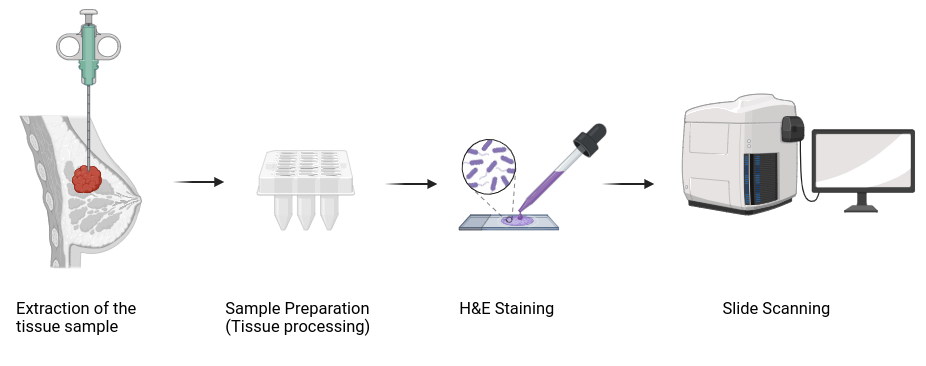
\includegraphics[width=\textwidth]{figures/slide_scanning_process.png}
    \caption{Slide Scanning process}
    \label{fig:slide_scanning_process}
\end{figure}

% general overview
\noindent This project aims to leverage computer vision and deep learning techniques to enhance the accuracy and efficiency of breast cancer diagnosis. By analyzing histopathological images of breast tissue samples, the goal is to develop a computer-aided diagnostic system capable of identifying malignant cells and distinguishing between different subtypes of breast cancer.
% challenges and objectives
Despite significant advancements in breast cancer diagnosis and treatment, several challenges persist in the field of medical AI. One general challenge is the annotation of histopathological images, which is a labor-intensive and time-consuming task requiring expert pathologists to accurately label the images. In our project, the main challenges were related to the size of the histopathological images (gigapixel images). These extremely high-resolution images result in substantial computational complexity, posing significant hardware challenges. Processing and analyzing such large images require considerable computational power and memory, which can be a limiting factor in developing efficient diagnostic systems.
The primary objective of this project, undertaken as part of the multidisciplinary project of our 2nd year of the second cycle at ESI SBA and our internship at CAC SBA (Centre Anti Cancer de Sidi Bel Abbes), is to develop a computer-aided diagnostic system capable of accurately classifying histopathological images of breast tissue into three classes: malignant, atypical, and benign. By training deep learning models to recognize and classify different histological features associated with these breast cancer subtypes, evaluating their performance, and integrating the diagnostic system into a workflow system specifically designed for CAC SBA, which includes a database for saving the necessary information of patients, we aim to support pathologists in their decision-making process. 
% Information system
We designed and developed an Information System (\acrshort{IS}), specifically a workflow system, tailored for CAC SBA (Centre Anti Cancer of Sidi Bel Abbes), to complement the development of the computer-aided diagnostic system for accurately classifying histopathological images of breast tissue. This workflow system serves the dual purpose of facilitating the collection and storage of necessary patient data, as well as automating the process of retrieving patient information. By seamlessly integrating the diagnostic system with the workflow system, the aim was to streamline the diagnostic process and enhance overall efficiency in breast cancer diagnosis at CAC SBA.

\newpage
\section{Background}

\subsection{Convolutional Neutral Networks}

\noindent Convolutional Neutral Networks (\acrshort{CNN}s : \autoref{fig:cnn-architecture}) are a type of deep learning architectures that made impressive achievements in various fields such as computer vision and natural language processing, a \acrshort{CNN} architecture mainly consists of : 

\begin{itemize}
    \item \textbf{Convolutional layers:} Responsible for extracting features from the input data.
    \item \textbf{Pooling layers:} Reduce the size of the feature maps while retaining the most important features.
    \item \textbf{Fully connected layers:} Responsible for decision making, as it takes the feature vector generated by previously mentioned layers and outputs class probabilities.
\end{itemize}.

\begin{figure}[H]
    \centering
    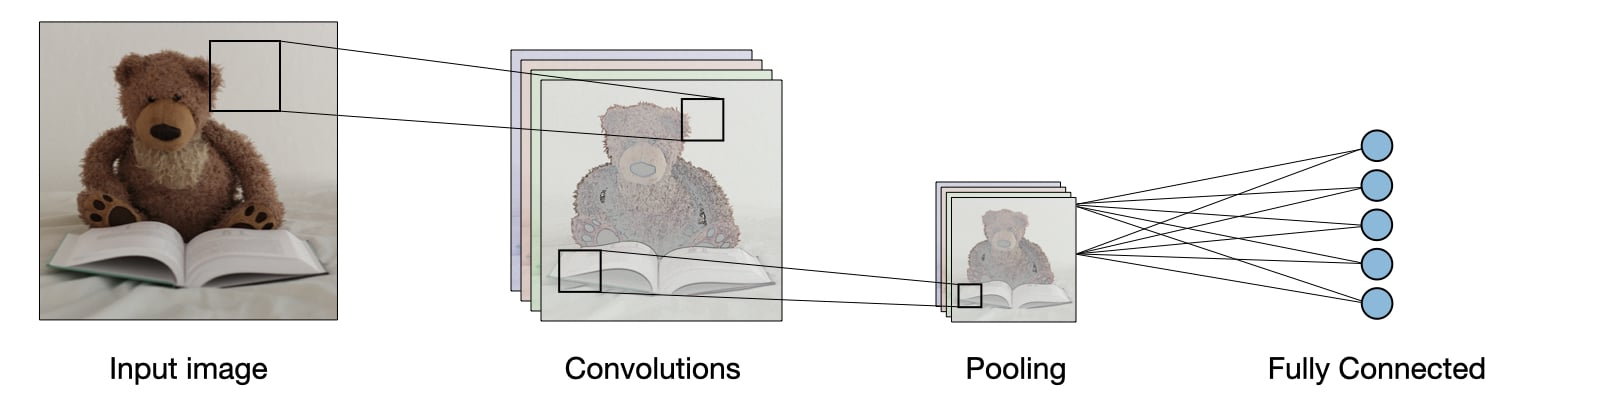
\includegraphics[width=0.8\textwidth]{figures/background/architecture-cnn-en.jpeg}
    \caption{Architecture of a traditional \acrshort{CNN} $^{\text{\cite{CNNs-stanford}}}$.}
    \label{fig:cnn-architecture}
\end{figure}

\subpar{Convolutional layers}

\noindent Convolutional layers provide a way to automatically extract features from the input data such as images. They consist of learnable filters (also called kernels) which have small widths and heights and the same depth as the input feature map (initially, it is the input image with a depth of 3 corresponding to the three channels R, G, and B).

\begin{itemize}
    \item During the forward pass, the layer processes its input patch by patch using a sliding window with a width and height identical to the filter's.
    \item Each time the window moves, it shifts by a particular number of pixels called the stride.
    \item The output is the dot product between the kernel weights and the patch.
    \item After repeating this process for each filter, we will stack their results to get a new feature map with a depth equal to the number of filters.
\end{itemize}

\begin{figure}[H]
    \centering
    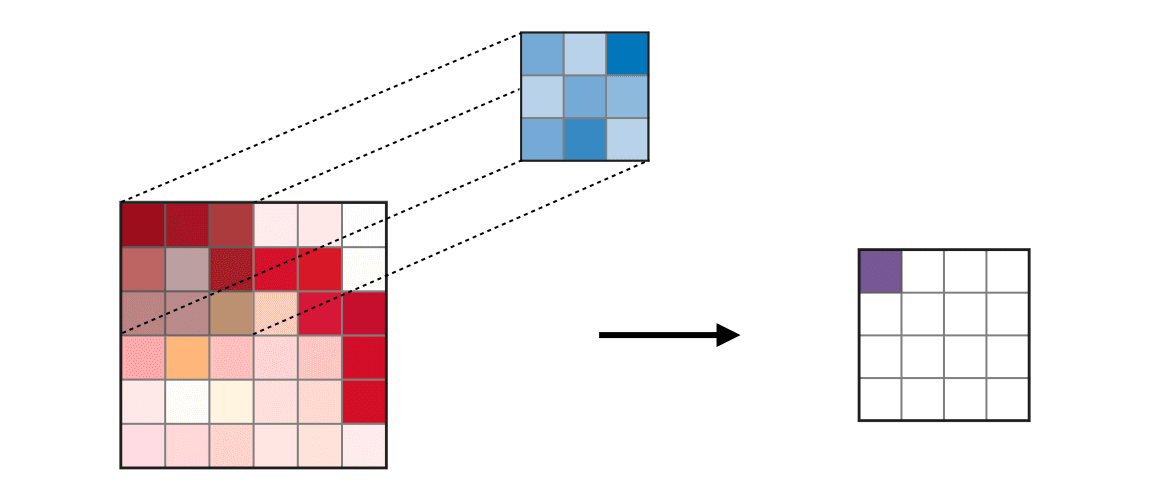
\includegraphics[width=0.6\textwidth]{figures/background/convolution-layer-a.png}
    \caption{Convolution layer $^{\text{\cite{CNNs-stanford}}}$.}
    \label{fig:convolutional-layer}
\end{figure}

\subpar{Pooling layers}

\noindent Pooling layers with no learnable parameters responsible for reducing the spatial dimensions of the input feature map, in terms of width and height, while retaining the most important information, several types of pooling layers exists including: .

\begin{itemize}
    \item \textbf{Max pooling:} takes the maximum of the region.
    \item \textbf{Average pooling:} takes the average of the region.
    \item \textbf{Global max pooling:} takes the maximum value over the entire feature map.
    \item \textbf{Global average pooling:} takes the average value over theentire feature map.
    \item \textbf{L2 pooling:} takes the L2 norm of each region.
    \item \textbf{Fractional max pooling:} takes the maximum value over a randomly chosen subset of the region.
\end{itemize}

\noindent The dimensions of the resulted feature map is calculated the same way as the convolutional layer,because pooling layers also process the input feature map using a moving window.

\begin{figure}[H]
    \centering
    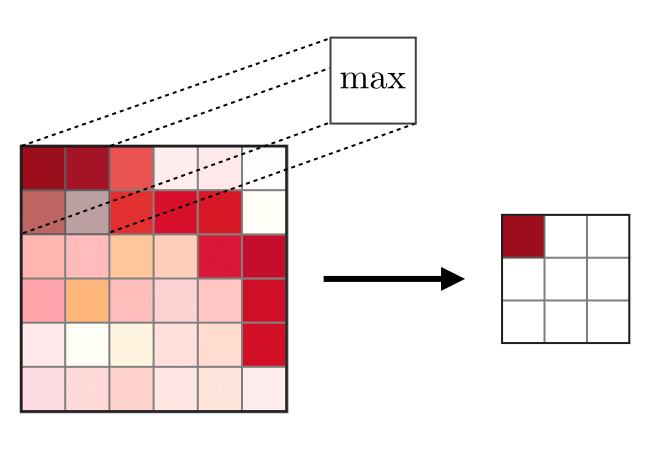
\includegraphics[width=0.45\textwidth]{figures/background/max-pooling-a.png}
    \caption{Max-Pooling layer in action $^{\text{\cite{CNNs-stanford}}}$.}
\end{figure}

\subsection{Residual Networks}

\noindent For complex tasks, deeper networks are preferable, but they present their own challenges, mainly computational complexity, which increases as more layers are added, and the ease of training, as it is proven that deeper networks are generally harder to optimize due to the problem of vanishing or exploding gradient descent.\\

\noindent Residual Networks $^{\text{\cite{BRACS_DATASET}}}$ (\acrshort{ResNet}) are a family of architectures that have been proven successful in image recognition tasks. They make use of the concept of deep residual learning, which is achieved using "shortcut connections" (\autoref{fig:shortcut-connection}) – the building block for this type of architecture – to ease the training and optimization of deeper networks with less computational complexity.\\

\begin{figure}[H]
    \begin{minipage}{0.4\textwidth}
        \centering
        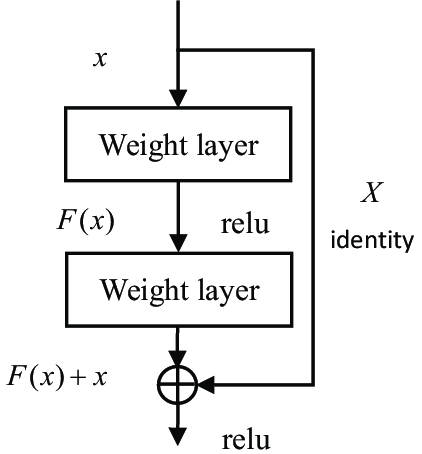
\includegraphics[width=0.625\textwidth]{figures/background/shortcut-connection.png}
    \end{minipage}
    \hfill
    \begin{minipage}{0.55\textwidth}
        \noindent
        A shortcut connection skips some of the layers in the neural network and feeds the output of one layer as the input to the next layers. In the case of \acrshort{ResNet}, the shortcut connections simply perform identity mapping, and their outputs are added to the outputs of the stacked layers. It is defined as:

        $$
        y = \mathcal{F}(x, \{W_{i}\}) + x
        $$
    \end{minipage}
    \captionsetup{justification=raggedright,singlelinecheck=false}
        \caption{Shortcut connection $^{\text{\cite{ResNet-OG}}}$.}
        \label{fig:shortcut-connection}
\end{figure}

\noindent \textbf{\acrshort{ResNet}18} (\autoref{fig:ResNet-18}) and \textbf{\acrshort{ResNet}34} (\autoref{fig:ResNet-34}) are two state-of-the-art residual networks for image classification tasks,they consist of 18 and 34 layers respectively including convolutional layers, batch normalization, and ReLU activation functions and one fully connected layer responsible for outputting classes probabilities. 

\begin{figure}[H]
     \centering
     \begin{subfigure}[b]{0.4\textwidth}
         \centering
         \includegraphics[width=0.5\textwidth]{figures/background/ResNet18.png}
         \caption{\acrshort{ResNet}-18 Architecture $^{\text{\cite{ResNet-OG}}}$}
         \label{fig:ResNet-18}
     \end{subfigure}
     \hfill
     \begin{subfigure}[b]{0.4\textwidth}
         \centering
         \includegraphics[width=0.5\textwidth]{figures/background/ResNet34.png}
         \caption{\acrshort{ResNet}-34 $^{\text{\cite{ResNet-OG}}}$.}
         \label{fig:ResNet-34}
     \end{subfigure}
\end{figure}

\newpage

\subsection{Attention mechanisms}

\noindent Attention mechanisms are deep learning techniques,emerged initially to improve computer vision and the encoder-decoder-based neural machine translation system,it is basically a dynamic weight adjustment function based on an attention function $g(x)$ and an input feature map $x$ that is superimposed between the convolutional layers. its role is to tell the next layer of the deep network which features are more or less important, this can be formulated as :.

$$
Attention = f(g(x), x)
$$

\noindent Here $g$ is responsible for generating attention which
corresponds to the process of attending to the discriminative
regions. $f(g(x), x)$ means processing input $x$ based on the
attention $g(x)$ to get more information.

\subsection{Vision transformers}

\noindent Building on the concept of attention, the transformer architecture $^{\text{\cite{AttIsAllYouNeed}}}$ was introduced,they rely entirely on self-attention mechanisms to process input data, dispensing with the recurrent structure of \acrshort{RNN}s. This allows transformers to handle long-range dependencies more efficiently and in parallel, leading to significant improvements in performance for tasks such as machine translation, text summarization, and beyond. Transformers have become the backbone of state-of-the-art models like \acrshort{BERT}, \acrshort{GPT}, and \acrshort{T5}.\\

\noindent Vision transformers $^\text{\cite{Vit}}$ (\acrshort{ViT}s \autoref{fig:vision-transformer}) are encoder-only transformers adapted for computer vision tasks. The idea is to break down an image of size $W \times H$ into a series of patches of size $P_w \times P_h$. These patches are then flattened, resulting in a two-dimensional matrix of dimensions $S \times D$, where $S = \frac{W}{P_w} \times \frac{H}{P_h}$ and $D = P_w \times P_h$. A linear projection layer is used to transform the individual flattened patches to a lower-dimensional vector, resulting in a matrix of dimension $S \times D'$. Finally, positional embedding is applied.\\

\noindent The output of patching and positional embedding is then fed to a regular transformer encoder,the outputs of the encoder are then passed to a Multi-Layer Perception to output the classes probabilities. 

\begin{figure}[H]
    \centering
    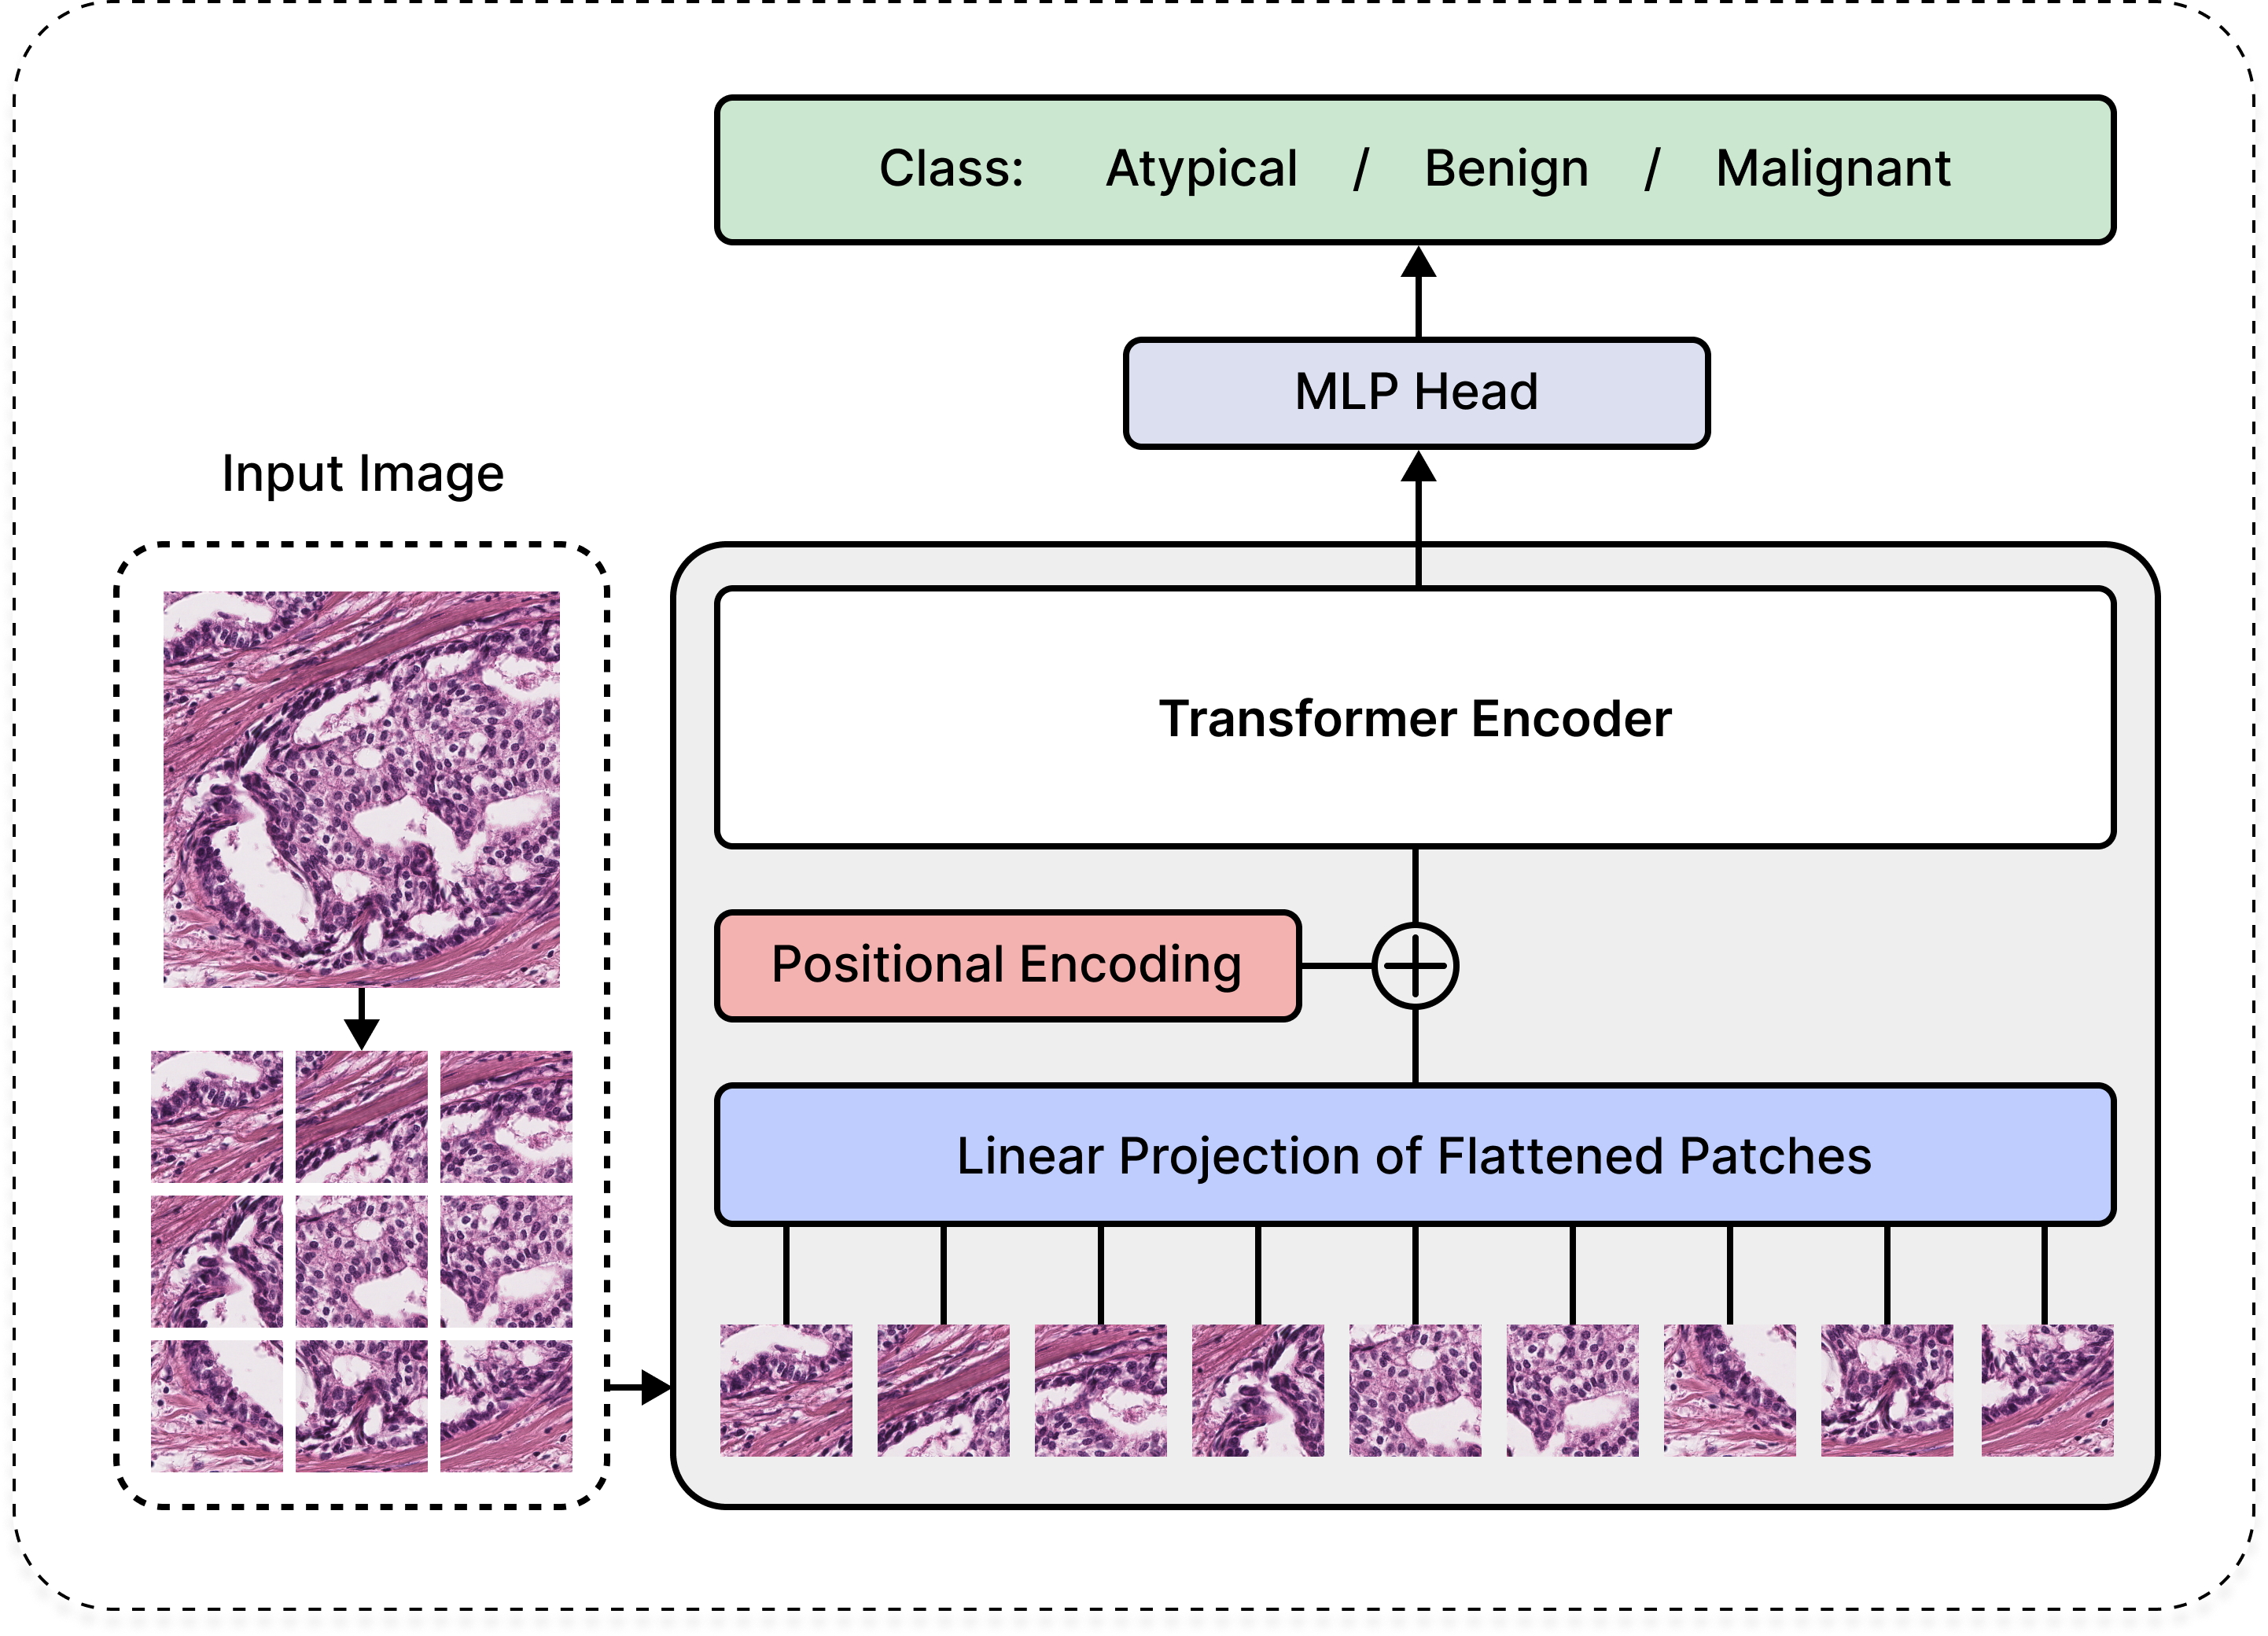
\includegraphics[width=0.65\textwidth]{figures/background/ViT.png}
    \caption{Vision Transformer architecture}
    \label{fig:vision-transformer}
\end{figure}

\subsection{Fine tuning \& transfer learning}

\noindent Fine-tuning and transfer learning are particular techniques in deep learning that allow reusing the knowledge learned from training a model on a certain task for other tasks. Both work by adapting a pre-trained model, which was trained on a more general task or another similar task, by retraining it on the new task.\\

\begin{figure}[H]
    \centering
    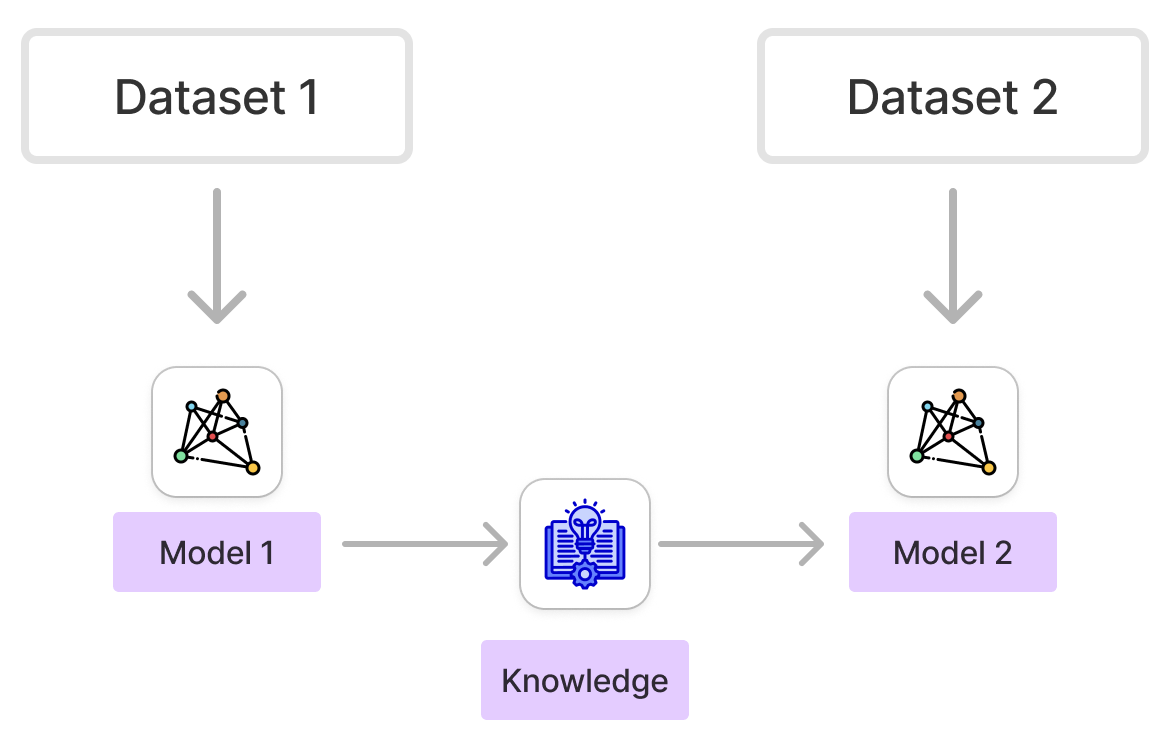
\includegraphics[width=0.6\textwidth]{figures/background/tl.png}
    \caption{The process of Fine tuning / transfer learning}
    \label{fig:transfer-learning-fine-tuning}
\end{figure}


\noindent Transfer learning utilizes the pre-trained model as a feature extractor, which means that the layers responsible for feature extraction, such as convolutional layers in computer vision, are frozen, while the decision-making layers, such as the last fully connected layers in \acrshort{CNN}s, are modified to match the task's nature and requirements, and only these decision-making layers are trained. Transfer learning is suitable when limited labeled data or computational resources are available, and there is a high similarity between the tasks.\\

\noindent In fine-tuning, we do not completely rely on the features learned from the source task but further "fine-tune" them to enhance the representation of our data and overcome potential differences between the source and the target task. This can be achieved by unfreezing some or all of the layers responsible for feature extraction, usually those closest to the decision-making layers, as they are responsible for extracting more fine-grained features, while earlier layers are responsible for extracting more low level features that similar tasks usually share,therfore fine tuning represents a more flexible way to re-use model as the number of layers to unfreeze have an impact on the model's performance and can be tweaked in function of the anount of available data,the similarity between the tasks and the computational resources.\\

\newpage
\subsection{Multi-instance learning}

\noindent Multi-instacne learning is a sub-type of supervised learning,where instead of associating a label with each data point,we associate a single label $Y$ with a set of data points called a bag $X = \{ x_{1},x_{2},...,x_{K} \}$, where $K$ is the size of the bag that could vary for different bags, in \acrshort{MIL} it is assumed that labels $\{y_{1},y_{2},...,y_{K}\}$ for individual instances exists, but they are unknown and that a bag may be labeled negative if all the instances in the bag are negative, or positive if there is at least one positive instance in the case of a binary classification problem, the assumption behind \acrshort{MIL} can be formulated as : 

$$
Y = \begin{cases}
    0 \text{ if } \sum\limits_{i=1}^{K} y_{i} = 0\\
    1 \text{ otherwise}
\end{cases}
$$

\noindent \acrshort{MIL} is particularly useful in scenarios where labeling individual instances is challenging or expensive, but labeling groups (bags) is feasible. Common applications include:

\begin{itemize}
    \item Medical Imaging: Identifying whether a medical image (bag) contains any instances of a disease (instance) without pinpointing the exact location of the disease.
    \item Text Categorization: Classifying documents (bags) based on whether they contain certain topics (instances), with each document being a collection of text segments or sentences.
    \item Drug Activity Prediction: Determining whether a molecule (bag) has a particular activity based on its conformations (instances).
\end{itemize}

\noindent There are several approaches to solving \acrshort{MIL} problems, each with its own strengths and weaknesses. Some common methods include:

\begin{itemize}
  \item Instance-based Approaches: These methods focus on the instances within the bags. A common technique involves assuming the presence of at least one positive instance in positive bags.
    \item Bag-based Approaches: These methods treat the entire bag as a single entity and attempt to classify it based on its overall characteristics.
  \item Embedded Space Approaches: These methods transform the bags into a different space where traditional machine learning algorithms can be applied.
\end{itemize}

\newpage
\section{State of the art}
 This section aims to provide an overview of the current state-of-the-art in deep learning-based approaches for breast cancer diagnosis through multi-classification of histology images.  Several studies have proposed CNN-based approaches \cite{CNNs} for breast cancer histology image classification. Attention models \cite{Att-Computer-Vision} and Vision Transformers \cite{Vit} have been explored as well. 
 \newline
In \cite{Structered-DL-Model} a CNN Class Structure-based approach was used on the Breast Cancer Histopathological (BreakHis) dataset \cite{BreakHis_DATASET}, in order to leverage the hierarchical feature representation. At the image level, an accuracy of about 92\% for all magnification factors was achieved in respect of a multi-classification in eight classes, and an approximate accuracy of 96\% was achieved for the binary classification. Another approach was presented in \cite{Classification_of_BRCA_hist_CNN}, where the performance was evaluated on the dataset provided by the Bioimaging 2015 challenge \cite{BIOIMAGING}. A CNN and a combination of a CNN and an SVM were proposed, achieving accuracies of 77.8\% for the four class test and 83.3\% for the carcinoma/non-carcinoma test.
\cite{brca-resnet-finetuning} presented a supervised method for the multi-classification of breast cancer histology images based on the fine-tuning strategy of a ResNet model \cite{ResNet-OG}. The classification of a breast cancer histology image has been obtained by combining three configurations of the ResNet with a different number of layers according to the maximum probability rule. The method has been tested on the Grand Challenge on Breast Cancer Histology Images (BACH) dataset \cite{BATCH}, and on the dataset provided by the Bioimaging 2015 challenge. Different experiments have been performed, using different training modalities of ResNet. The best accuracy was obtained by applying the fine-tuning strategy,
training all the layers of the networks. The accuracy achieved was 97.3\% for the multi-classification in four classes and 98.7\% for carcinoma/non-carcinoma test on the BACH dataset.
 To reduce the training parameters  and reduce the risk of model over-fitting, \cite{SE-RESNET} designed a small SE-ResNet model based on the combination of residual module and Squeeze-and-Excitation block. Compared to the bottleneck SE-ResNet module and basic SE-ResNet module, the parameters of the small SE-ResNet module is reduced to 29.4\% and 33.3\%, respectively. The authors also proposed a new learning rate scheduler named Gaussian error scheduler which can get excellent performance without complicatedly fine-tuning the learning rate. Additionally they designed a novel CNN network based on small SE-ResNet module, pooling layer, and fully connected layer. This model has been tested on the BreakHis dataset for binary classification and multi-class classification with competitive experimental results. Accuracies of 93.74\%, 93.81\%, 92.22\%, and 90.66\% have been acheived on the multi-classification task. 
\cite{Gigapixel} proposed a framework that consists of two stages: a Grid-based Feature Extraction (GFE) and an Attention-based Classifier (AC). The GFE applies a CNN to extract patch-wise features and aggregate feature vectors in a compact grid representation according to the spatial location of the corresponding patches in the WSI. The AC implements both the min- and max-attention mechanisms separately on the input grid-based feature map and produces two different sets of attention maps. The attention maps are then used for classification. \cite{HIPT} proposed a framework named  Hierarchical Image Pyramid Transformer (HIPT). This work aimed to adapt ViTs \cite{Vit} for slide-level representation learning to capture the hierarchical structure of WSIs. ViT256 -16, ViT4096 -256 and ViTWSI -4096 have been proposed and utilized to aggregate visual tokens at different levels to form slide representations. The [CLS] tokens from ViT256 -16 are used as the input sequence for ViT4096 -256, with the [CLS] tokens from ViT4096 -256 subsequently used as the input sequence for ViTWSI -4096.

\newpage 
Below a comparative table the mentioned approaches:

\begin{table}[h]
    \centering
    \footnotesize % Further reduce the font size
    \begin{tblr}{colspec={|X[0.4]|X[0.8]|X[1.0]|X[1.3]|X[0.5]|}, hlines, stretch=1.1}
        Reference & DL Technique & Dataset & Results & Multiple Instance Learning \\
        \cite{Structered-DL-Model} &  Class structure-based deep convolutional neural network (CSDCNN) for the classification task. & BreakHis & - multi classification accuracy: 92\% \newline - binary classification accuracy: 96\% & No \\
        \cite{Classification_of_BRCA_hist_CNN} & Convolutional Neural Networks (CNNs) for feature extraction + SVM for classification. & Bioimaging 2015 challenge dataset & - multi classification accuracy: 77.8\% \newline - binary classification accuracy: 83.3\% & Yes \\
        \cite{brca-resnet-finetuning} & Fine tuning strategy on ResNet model & - BACH: Grand Challenge on Breast Cancer Histology Images. \newline - Bioimaging 2015 challenge dataset & - multi classification accuracy on Bioimaging 2015 challenge dataset: 97.2\% \newline - multi classification accuracy on BACH dataset: 97.3\% & No \\
        \cite{SE-RESNET} & - small SE-ResNet \newline - learning rate scheduler named Gaussian error scheduler \newline - novel CNN network based on small SE-ResNet module & BreakHis & - multi classification accuracy: 90.66\% and 93.81\% \newline - binary classification accuracy: 98.87\% and 99.34\% & Yes \\
        \cite{Gigapixel} & - a Grid-based Feature Extraction (CNN) \newline - Attention-based Classifier & - Camelyon16 \newline - TUPAC16 & - Prediction of Metastasis presence AUC: 0.711 \newline - Prediction of Tumor Proliferation Speed, spearman correlation coefficient: 0.662-0.653 & Yes \\
        \cite{HIPT} & - Adapting ViTs. \newline - Hierarchical Self-Supervised Learning & TCGA & - 0.821-0.874 AUC on BRCA subtyping & Yes \\
    \end{tblr}
    \caption{Comparative table of state of the art methods}
    \label{tab:state_of_the_art_summary}
\end{table}



\newpage
\section{\acrshort{BRACS} Dataset}
BReAst Carcinoma Subtyping (\acrshort{BRACS}) dataset $^{\text{\cite{BRACS_DATASET}}}$, a large cohort of annotated Hematoxylin and Eosin (\acrshort{HE})-stained images to facilitate the characterization of breast lesions.\\

\noindent The dataset was built through the collaboration of the National Cancer Institute—Scientific Institute for Research, Hospitalization and Healthcare (\acrshort{IRCCS}) ‘Fondazione G. Pascale’, the Institute for High Performance Computing and Networking (\acrshort{ICAR}) of National Research Council (\acrshort{CNR}) and International Business Machines (IBM) Research—Zurich. The dataset was acquired from patients between 2019 and 2020, by board-certified clin-icians of the Department of Pathology at the National Cancer Institute—\acrshort{IRCCS} ‘Fondazione G. Pascale’ in Naples (Italy).\\

\noindent The \acrshort{BRACS} dataset comprises both Whole Slide Images (\acrshort{WSI}s) and Regions of Interest (\acrshort{ROI}s). \acrshort{WSI}s are digital images of entire histological slides, capturing the complete tissue section at high resolution (Gigapixels), and they have been obtained by scanning slides that were selected by a biologist of the pathological anatomy department. Regions of Interest (\acrshort{ROI}s), on the other hand, represent carefully selected and annotated image patches that were extracted from the Whole Slide Images (\acrshort{WSI}s), focusing on specific areas of interest within the vast expanse of the \acrshort{WSI}s.\\

\subsection{Data collection and annotation process}
The samples were obtained from hematoxylin and eosin (\acrshort{HE}) stained breast tissue biopsy slides, with the selection based on the diagnostic reports of the patients. The age distribution of the patients ranged from \textbf{16} to \textbf{86} years, with approximately \textbf{61\%} of the patients falling within the \textbf{40–60} age range and only a few patients under \textbf{20} or over \textbf{80} years old.\\

\noindent A Whole Slide Image (\acrshort{WSI}) typically includes several lesions of varying subtypes, including Normal \textbf{(\acrshort{N})}, Pathological Benign \textbf{(\acrshort{PB})}, Usual Ductal Hyperplasia \textbf{(\acrshort{UDH})}, Flat Epithelial Atypia \textbf{(\acrshort{FEA})}, Atypical Ductal Hyperplasia \textbf{(\acrshort{ADH})}, Ductal Carcinoma in Situ \textbf{(\acrshort{DCIS})}, and Invasive Carcinoma \textbf{(\acrshort{IC})}. To ensure a high level of reliability in the annotations, three expert pathologists were involved in annotating both the \acrshort{WSI}s and Regions of Interest (\acrshort{ROI}s).\\

\noindent Initially, each pathologist inspected the \acrshort{WSI}s, assigning the corresponding label according to the most aggressive tumor subtype they detected within the image. After that, all annotations were collectively reviewed by the three pathologists, and those with disagreement were further discussed and re-annotated when consensus was reached or discarded otherwise.\\

\noindent A subset of the annotated \acrshort{WSI}s was split into three disjoint subsets, each of which was assigned to one of the pathologists. Each pathologist extracted a set of \acrshort{ROI}s from their assigned subset, while ensuring that at least one \acrshort{ROI} with the same subtype as the \acrshort{WSI} was selected and that the set of extracted \acrshort{ROI}s maintained a balanced distribution across the classes.\\

\subsection{Dataset characteristics}
The \acrshort{BRACS} dataset comprises a total of \textbf{547 \acrshort{WSI}s} obtained from \textbf{189 different patients}. The dataset also includes \textbf{4,539 \acrshort{ROI}s} that were extracted from \textbf{387 \acrshort{WSI}s} collected from \textbf{151 patients}. 
All slides in the dataset were scanned using an \textbf{Aperio AT2} scanner, which helps to capture images at a high resolution of \textbf{0.25 $\mu\mathrm{m}/\mathrm{pixel}$}. The scanning process used a magnification factor of \textbf{40x}, which ensured detailed imaging of the tissue samples. \autoref{tab:data_distribution} reports the distribution of \acrshort{WSI}s (with and without \acrshort{ROI}s) and \acrshort{ROI}s according to the lesion types and subtypes.\\

\begin{table}[ht]
    \centering
    \small
    \begin{adjustbox}{max width=\textwidth} % scale the table to fit within text width
        \begin{tabular}{@{}l|rrr|rrrrrrr@{}}
            \toprule
            & \multicolumn{3}{c|}{Types} & \multicolumn{7}{c}{Subtypes} \\
            \cmidrule(l){2-4} \cmidrule(l){5-11}
            Data & Benign & Atypical & Malignant & \acrshort{N} & \acrshort{PB} & \acrshort{UDH} & \acrshort{FEA} & \acrshort{ADH} & \acrshort{DCIS} & \acrshort{IC} \\
            \midrule
            \acrshort{WSI}s with \acrshort{ROI}s & 149 & 75 & 163 & 17 & 77 & 55 & 34 & 41 & 51 & 112 \\
            \acrshort{WSI}s without \acrshort{ROI}s & 116 & 14 & 30 & 27 & 70 & 19 & 7 & 7 & 10 & 20 \\
            \acrshort{WSI}s & 265 & 89 & 193 & 44 & 147 & 74 & 41 & 48 & 61 & 132 \\
            \acrshort{ROI}s & 1837 & 1263 & 1439 & 484 & 836 & 517 & 756 & 507 & 790 & 649 \\
            \bottomrule
        \end{tabular}
    \end{adjustbox}
    \caption{\acrshort{BRACS} data distribution according to lesion types and subtypes.}
    \label{tab:data_distribution}
\end{table}

\subsection{Dataset organization}
\acrshort{BRACS} dataset provides pre-defined \acrshort{WSI}- and \acrshort{ROI}-level splits in train, validation and test sets. Data split was generated such that all the \acrshort{WSI}s extracted from a patient belong to the same set. Similarly, all the \acrshort{ROI}s extracted in a given \acrshort{WSI} are assigned to the same split.  \autoref{tab:splits_distrib} reports the number of \acrshort{WSI}s and \acrshort{ROI}s included in the train, validation and test splits according to the lesion types.

\begin{table}[ht]
    \centering
    \small
    \begin{adjustbox}{max width=\textwidth} % scale the table to fit within text width
        \begin{tabular}{@{}l|rrrr|rrrr@{}}
            \toprule
            & \multicolumn{4}{c|}{\acrshort{WSI}-level split} & \multicolumn{4}{c}{\acrshort{ROI}-level split} \\
            \cmidrule(l){2-5} \cmidrule(l){6-9}
            Data & Benign & Atypical & Malignant & Total & Benign & Atypical & Malignant & Total \\
            \midrule
            Train & 203 & 52 & 140 & 395 & 1460 & 1011 & 1186 & 3657 \\
            Validation & 30 & 14 & 21 & 67 & 135 & 90 & 87 & 312 \\
            Test & 32 & 23 & 32 & 85 & 242 & 162 & 166 & 570 \\
            \midrule
            Total & 265 & 89 & 193 & \textbf{547} & 1837 & 1263 & 1439 & \textbf{4539}\\
            \bottomrule
        \end{tabular}
    \end{adjustbox}
    \caption{\acrshort{WSI}- and \acrshort{ROI}-level split according to the lesion types.}
    \label{tab:splits_distrib}
\end{table}

\noindent While \autoref{tab:splits2_distribution} reports the number of \acrshort{WSI}s and \acrshort{ROI}s included in the train, validation and test splits according to the lesion subtypes.

\begin{table}[ht]
    \centering
    \small
    \begin{adjustbox}{max width=\textwidth} % scale the table to fit within text width
        \begin{tabular}{@{}l|rrrrrrr|rrrrrrr@{}}
            \toprule
            & \multicolumn{7}{c|}{\acrshort{WSI}-level split} & \multicolumn{7}{c}{\acrshort{ROI}-level split} \\
            \cmidrule(l){2-8} \cmidrule(l){9-15}
            Data & \acrshort{N} & \acrshort{PB} & \acrshort{UDH} & \acrshort{FEA} & \acrshort{ADH} & \acrshort{DCIS} & \acrshort{IC} & \acrshort{N} & \acrshort{PB} & \acrshort{UDH} & \acrshort{FEA} & \acrshort{ADH} & \acrshort{DCIS} & \acrshort{IC} \\
            \midrule
            Train & 27 & 120 & 56 & 24 & 28 & 40 & 100 & 357 & 714 & 389 & 624 & 387 & 665 & 521 \\
            Validation & 10 & 11 & 9 & 6 & 8 & 9 & 12 & 46 & 43 & 46 & 49 & 41 & 40 & 47 \\
            Test & 7 & 16 & 9 & 11 & 12 & 12 & 20 & 81 & 79 & 82 & 83 & 79 & 85 & 81 \\
            \midrule
            Total & 44 & 147 & 74 & 41 & 48 & 61 & 132 & 484 & 836 & 512 & 756 & 507 & 790 & 649 \\
            \bottomrule
        \end{tabular}
    \end{adjustbox}
    \caption{\acrshort{WSI}- and \acrshort{ROI}-level split according to the lesion subtypes.}
    \label{tab:splits2_distribution}
\end{table}

\noindent The dataset is organized as follows. The \acrshort{WSI}s are stored in the 'Whole Slide Images Set' folder, which is further partitioned into train, validation, and test data subsets. Each of these subsets is divided into Benign (\acrshort{BT}), Atypical (\acrshort{AT}), and Malignant (\acrshort{MT}) folders, each containing folders corresponding to specific lesion subtypes. The \acrshort{WSI}s are saved as '.svs' files, adhering to a consistent naming convention. \\
On the other hand, the \acrshort{ROI}s are stored in the ‘Region of Interest Set’ folder, which follows the same structure as the \acrshort{WSI} set. The \acrshort{ROI} files are stored in png format. Finally, a summary file in '.xlsx' format is included, which lists for each \acrshort{WSI}s its label, data split assignment (train/validation/test), associated patient \acrshort{ID}, and the number of corresponding \acrshort{ROI}s, if there is any. \autoref{fig:data_organization} highlights the folder organization of \acrshort{BRACS} dataset.

\begin{figure}[H]
    \centering
    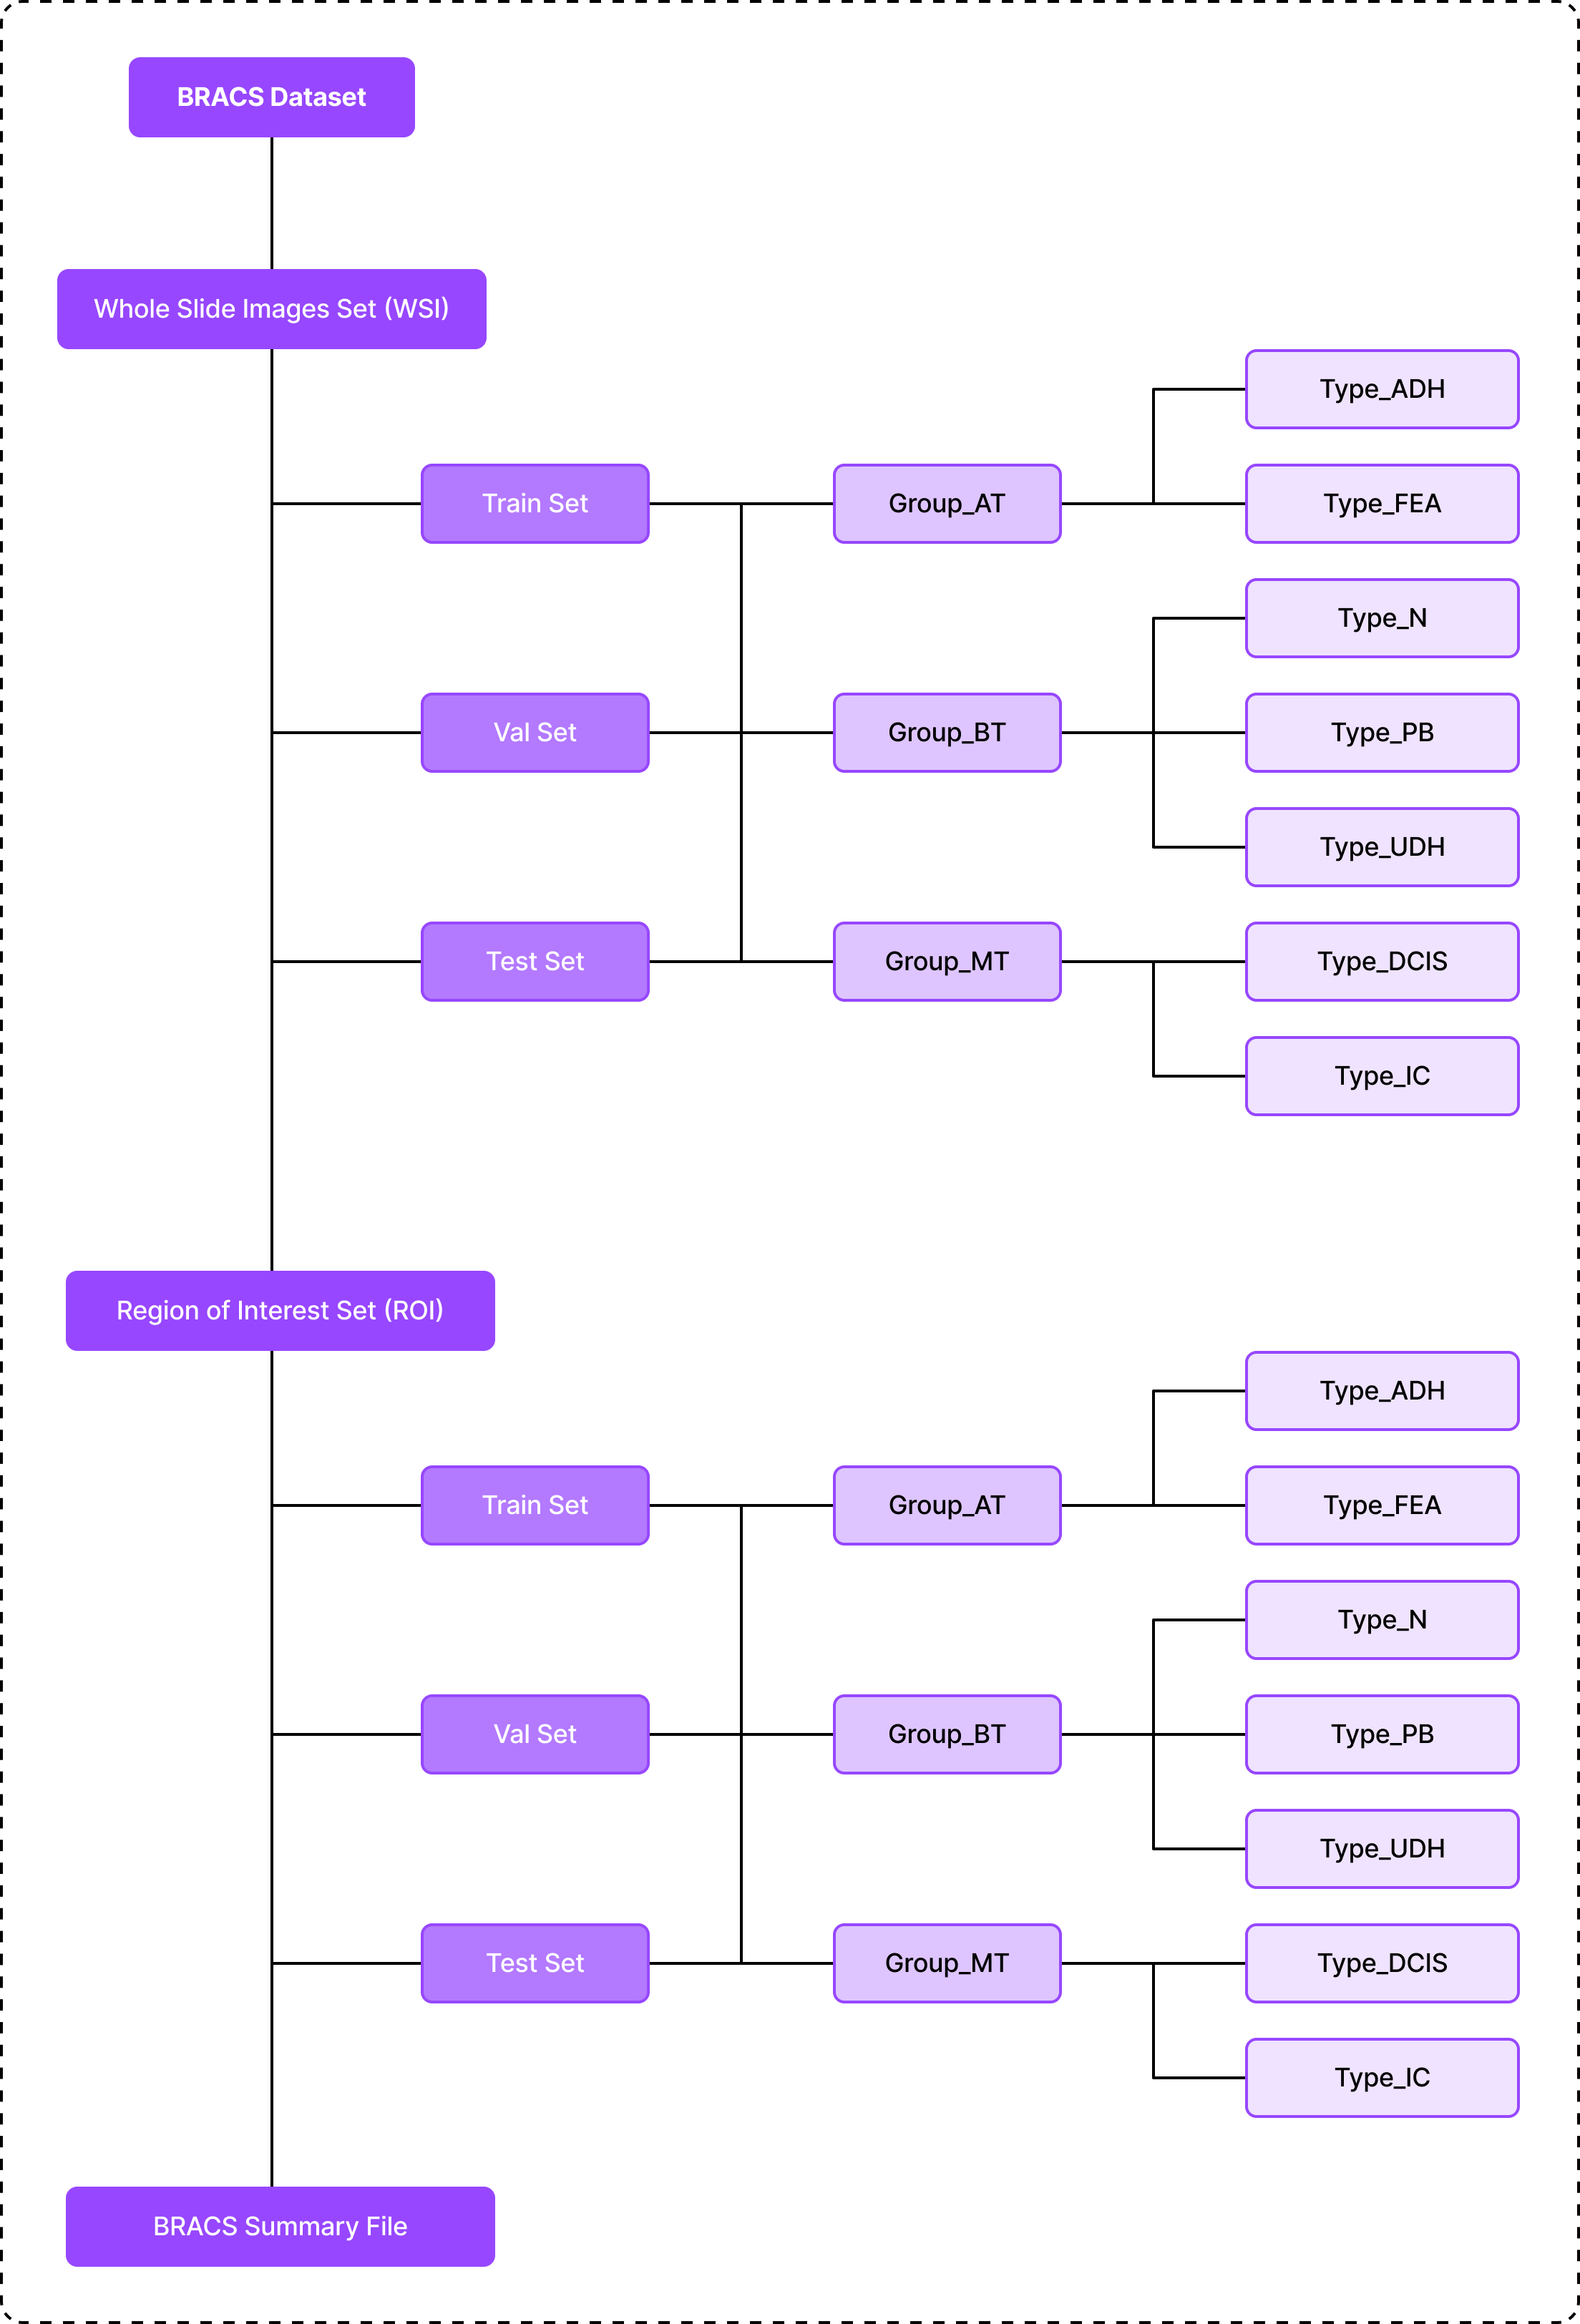
\includegraphics[width=0.75\textwidth]{figures/dataset/data_org.png}
    \caption{The organization of \acrshort{BRACS} dataset folders $^{\text{\cite{BRACS_DATASET}}}$.}
    \label{fig:data_organization}
\end{figure}

\newpage
\section{Approach}

\noindent Due to the computational challenges posed by gigapixel images and limited hardware and $\text{\acrshort{GPU}}$ $\text{\acrshort{RAM}}$, a two-step approach was adopted to overcome these challenges. In the first step, a feature extraction process takes place, where we process the $\text{\acrshort{WSI}}$ using the \textbf{OpenSlide} library to partially load the image and then process it through a pre-trained neural network to produce a more compact representation of the $\text{\acrshort{WSI}}$ that can be easily processed by the attention models. The second step involves training the attention models using the generated tensors from the first step. Two architectures were chosen: a \textbf{Min-Max Attention Classifier} $^\text{\cite{Gigapixel}}$ and a \textbf{Multi-Branch Attention Challenging Classifier}$^\text{\cite{ACMIL}}$. In the feature extraction step, we experimented with four different models: \textbf{\acrshort{ResNet}-18, \acrshort{ResNet}-34} (fine-tuned on $\text{\acrshort{BRACS}'}$ regions of interest), \textbf{\acrshort{ResNet}-50} (trained on Kather100k Dataset) and a \textbf{ViT-S/16} pre-trained using $\text{\acrshort{DINO}}$ on a substantial collection of $36,666$ $\text{\acrshort{WSI}s}$. \autoref{fig:approach} shows a schematic representation of the general approach.\\

\begin{figure}[H]
    \centering
    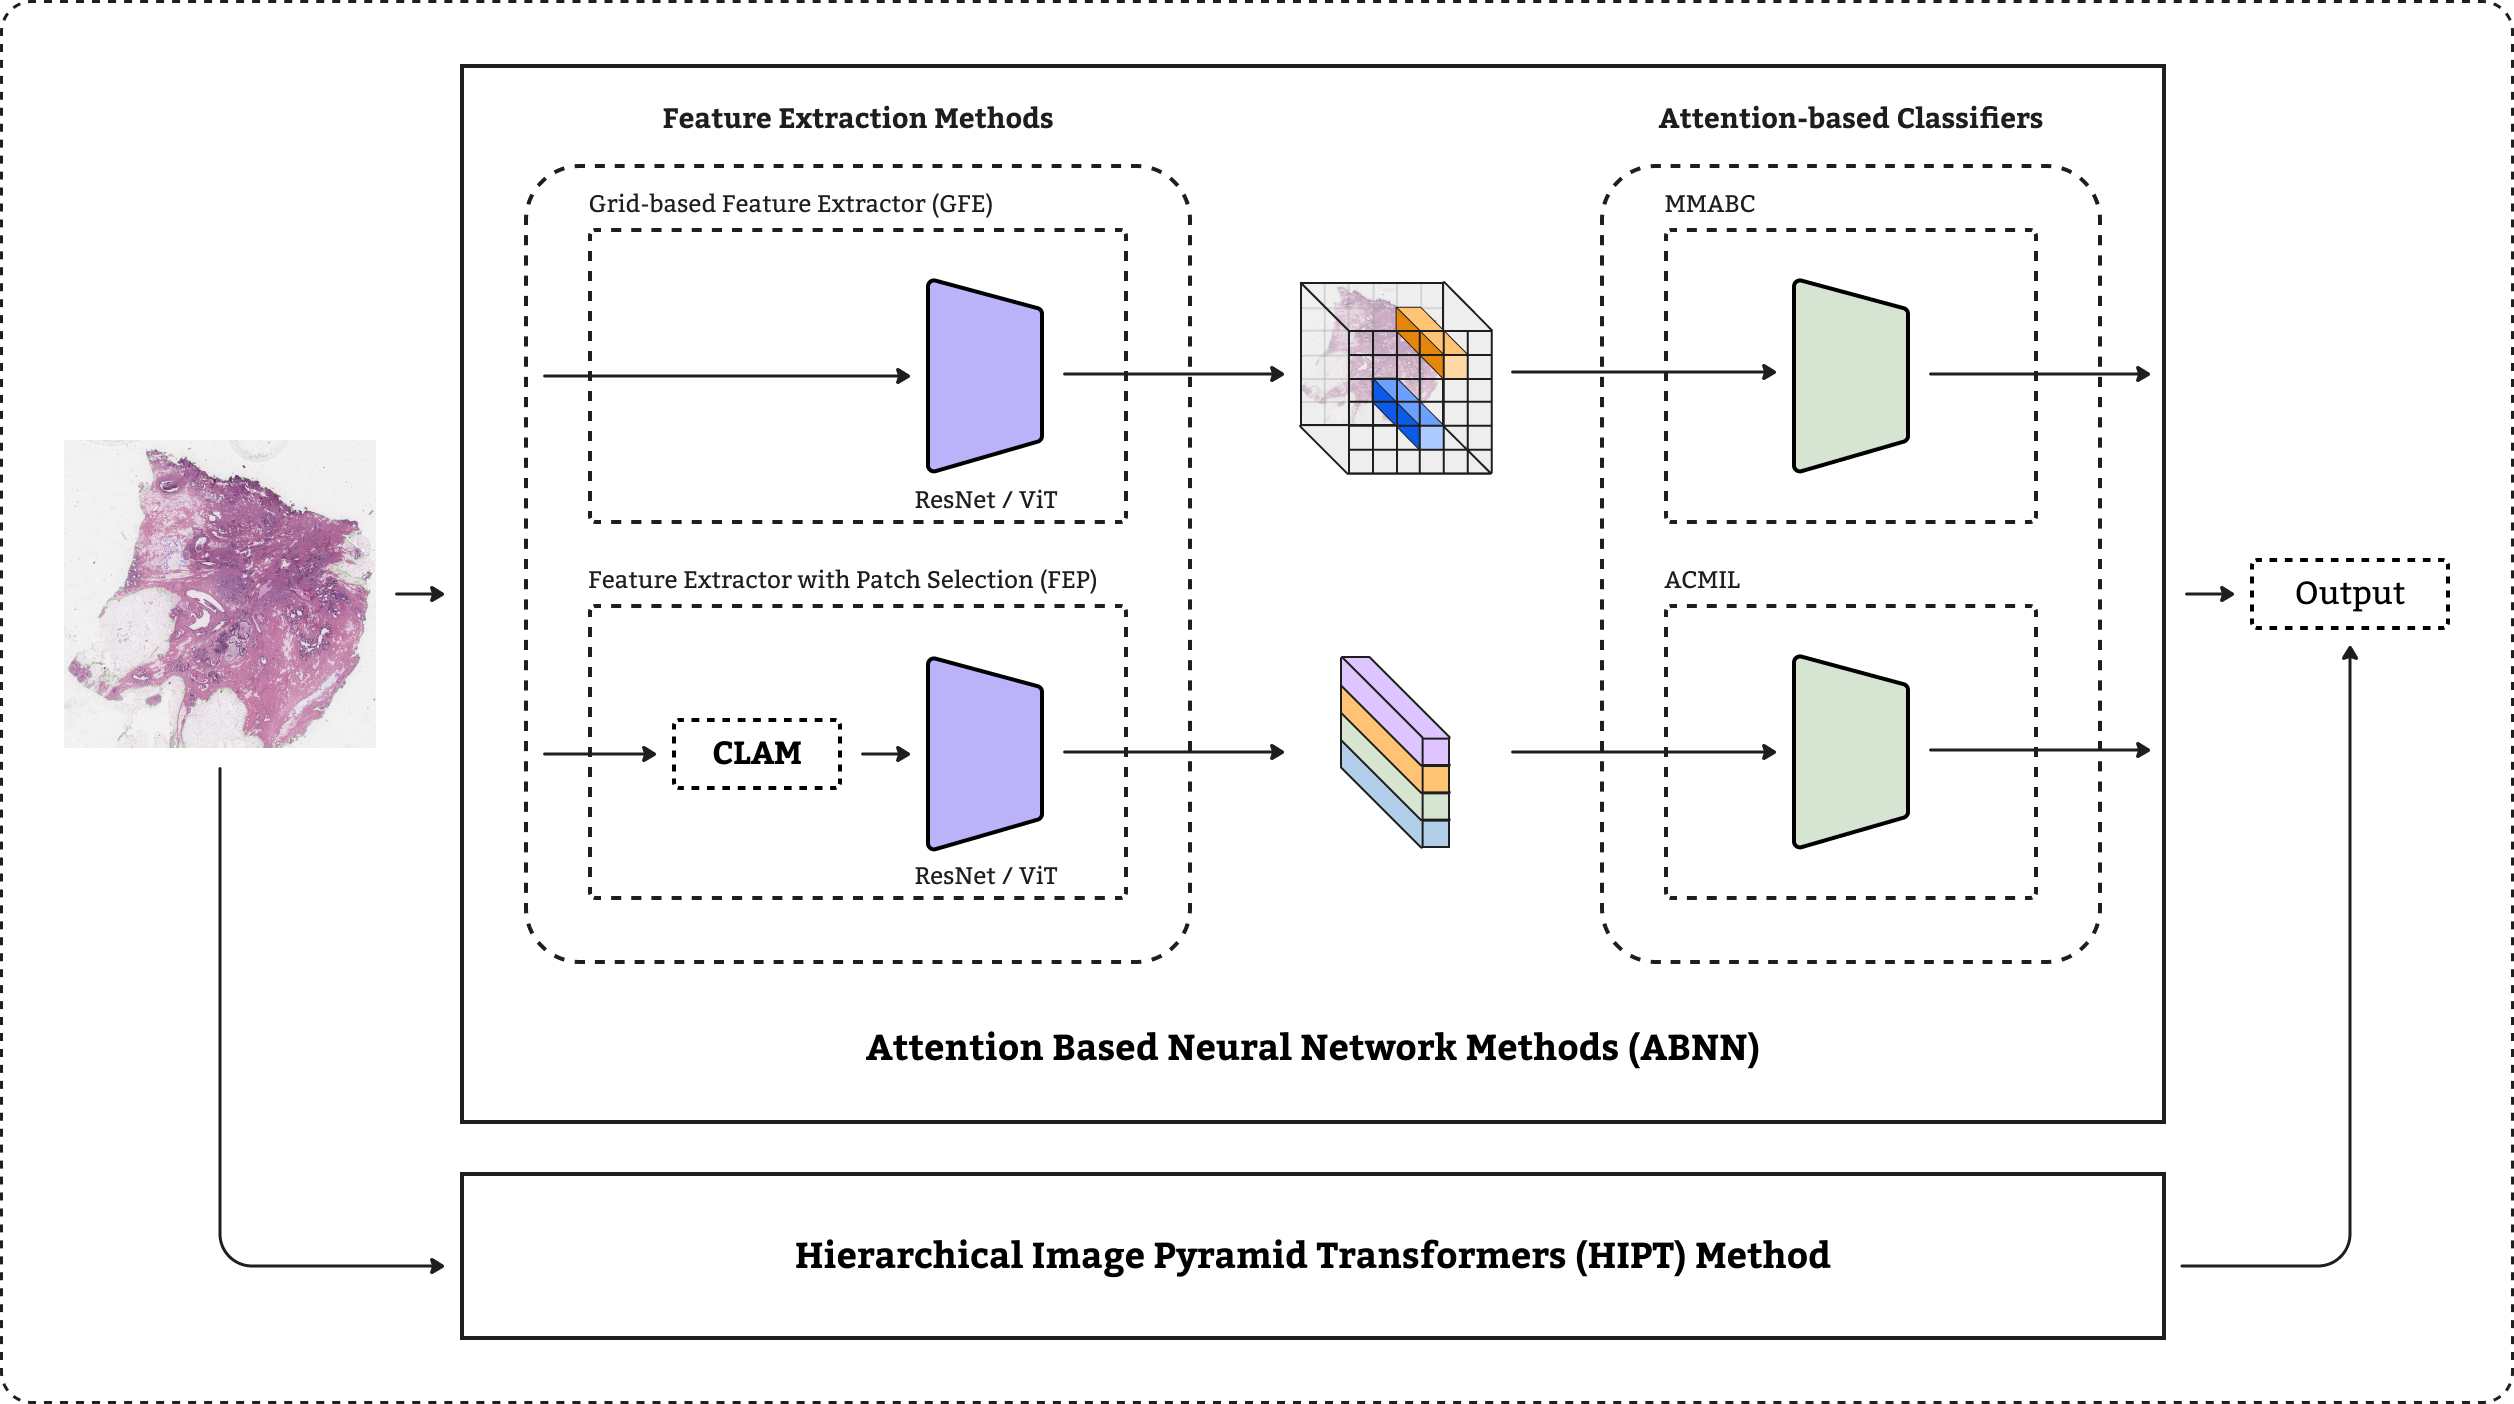
\includegraphics[width=\textwidth]{figures/approach.png}
    \caption{Schematic representation of the general approach.}
    \label{fig:approach}
\end{figure}

\noindent A high-level overview of the process is as follows :

\begin{itemize}
    \item Dividing the \acrshort{WSI} into a set of non-overlapping patches.
    $$
        X = \{x_{1},x_{2},...,x_{K}\}
    $$
    \item Pass the patches to a pre-trained neutral network to transform the patch into a low-dimensional embedding     
    $$
        h_{i} = f(x_{i})
    $$.
    \item Use an attention mechanism to generate a bag-level representation of the \acrshort{WSI} .
    $$
        \begin{cases}
            z = \sum\limits_{i=1}^{K} a_{i} * h_{i}\\
            a_{i} = \sigma(h_{n})
        \end{cases}
    $$.
    \item Generate the \acrshort{WSI} prediction from the bag-level representation.

    $$
        \hat{Y} = g(z)
    $$
    
\end{itemize}

\noindent Similarly, fine-tuning the \textbf{\acrshort{HIPT}} model was divided into two steps due to computational limitations. As explained earlier, the standard approach when applying fine-tuning or transfer learning is to load a pre-trained model's weights and initialize your architecture with those weights. Then, you can optionally freeze a number of layers and retrain the model on your own task. However, since it is impossible to load the entire \acrshort{WSI} into the \acrshort{GPU}'s memory, and the time it takes for it to propagate through the network's layers, even if partial loading was used to overcome the memory challenge, a similar approach was adopted. We processed the entire dataset using the frozen layers and saved their output to the disk, which would be the input to the part of the network we wished to train. The only drawback is that we cannot apply data augmentation to the input on-the-fly, and due to the spatial and time complexity challenges that the dataset possesses, iterating multiple times through the dataset and saving an augmented version of it is not an option. To overcome this drawback, we applied on-the-fly data augmentation on the generated tensors instead. Since the tensors have a shape of $W \times H \times C$, some of the usual data augmentation techniques used in computer vision were used, but re-implemented to work on an arbitrary number of channels.

\subsection{Preparing Models For Feature Extraction}

\noindent In the context of our project, it involves using pre-trained models and fine-tuning them on \acrshort{ROI} images, which are specific areas of \acrshort{WSI}s that contain significant diagnostic information selected by experts. By fine-tuning on these carefully selected regions, the models learn to identify critical patterns and features associated with cancerous tissues. This specialized training enables the models to become highly adept at recognizing the subtle distinctions necessary for accurate cancer detection. The fine-tuned models are then used as feature extractors for the entire \acrshort{WSI}s, allowing for a more efficient and specialized analysis. This approach maximizes the utility of annotated data, enhances the model's sensitivity to relevant pathological features, and ultimately improves the accuracy and reliability of cancer diagnosis in large-scale histopathological images. \autoref{fig:fine_tuning} illustrates the fine-tuning process on \acrshort{ROI} images.

\begin{figure}[H]
    \centering
    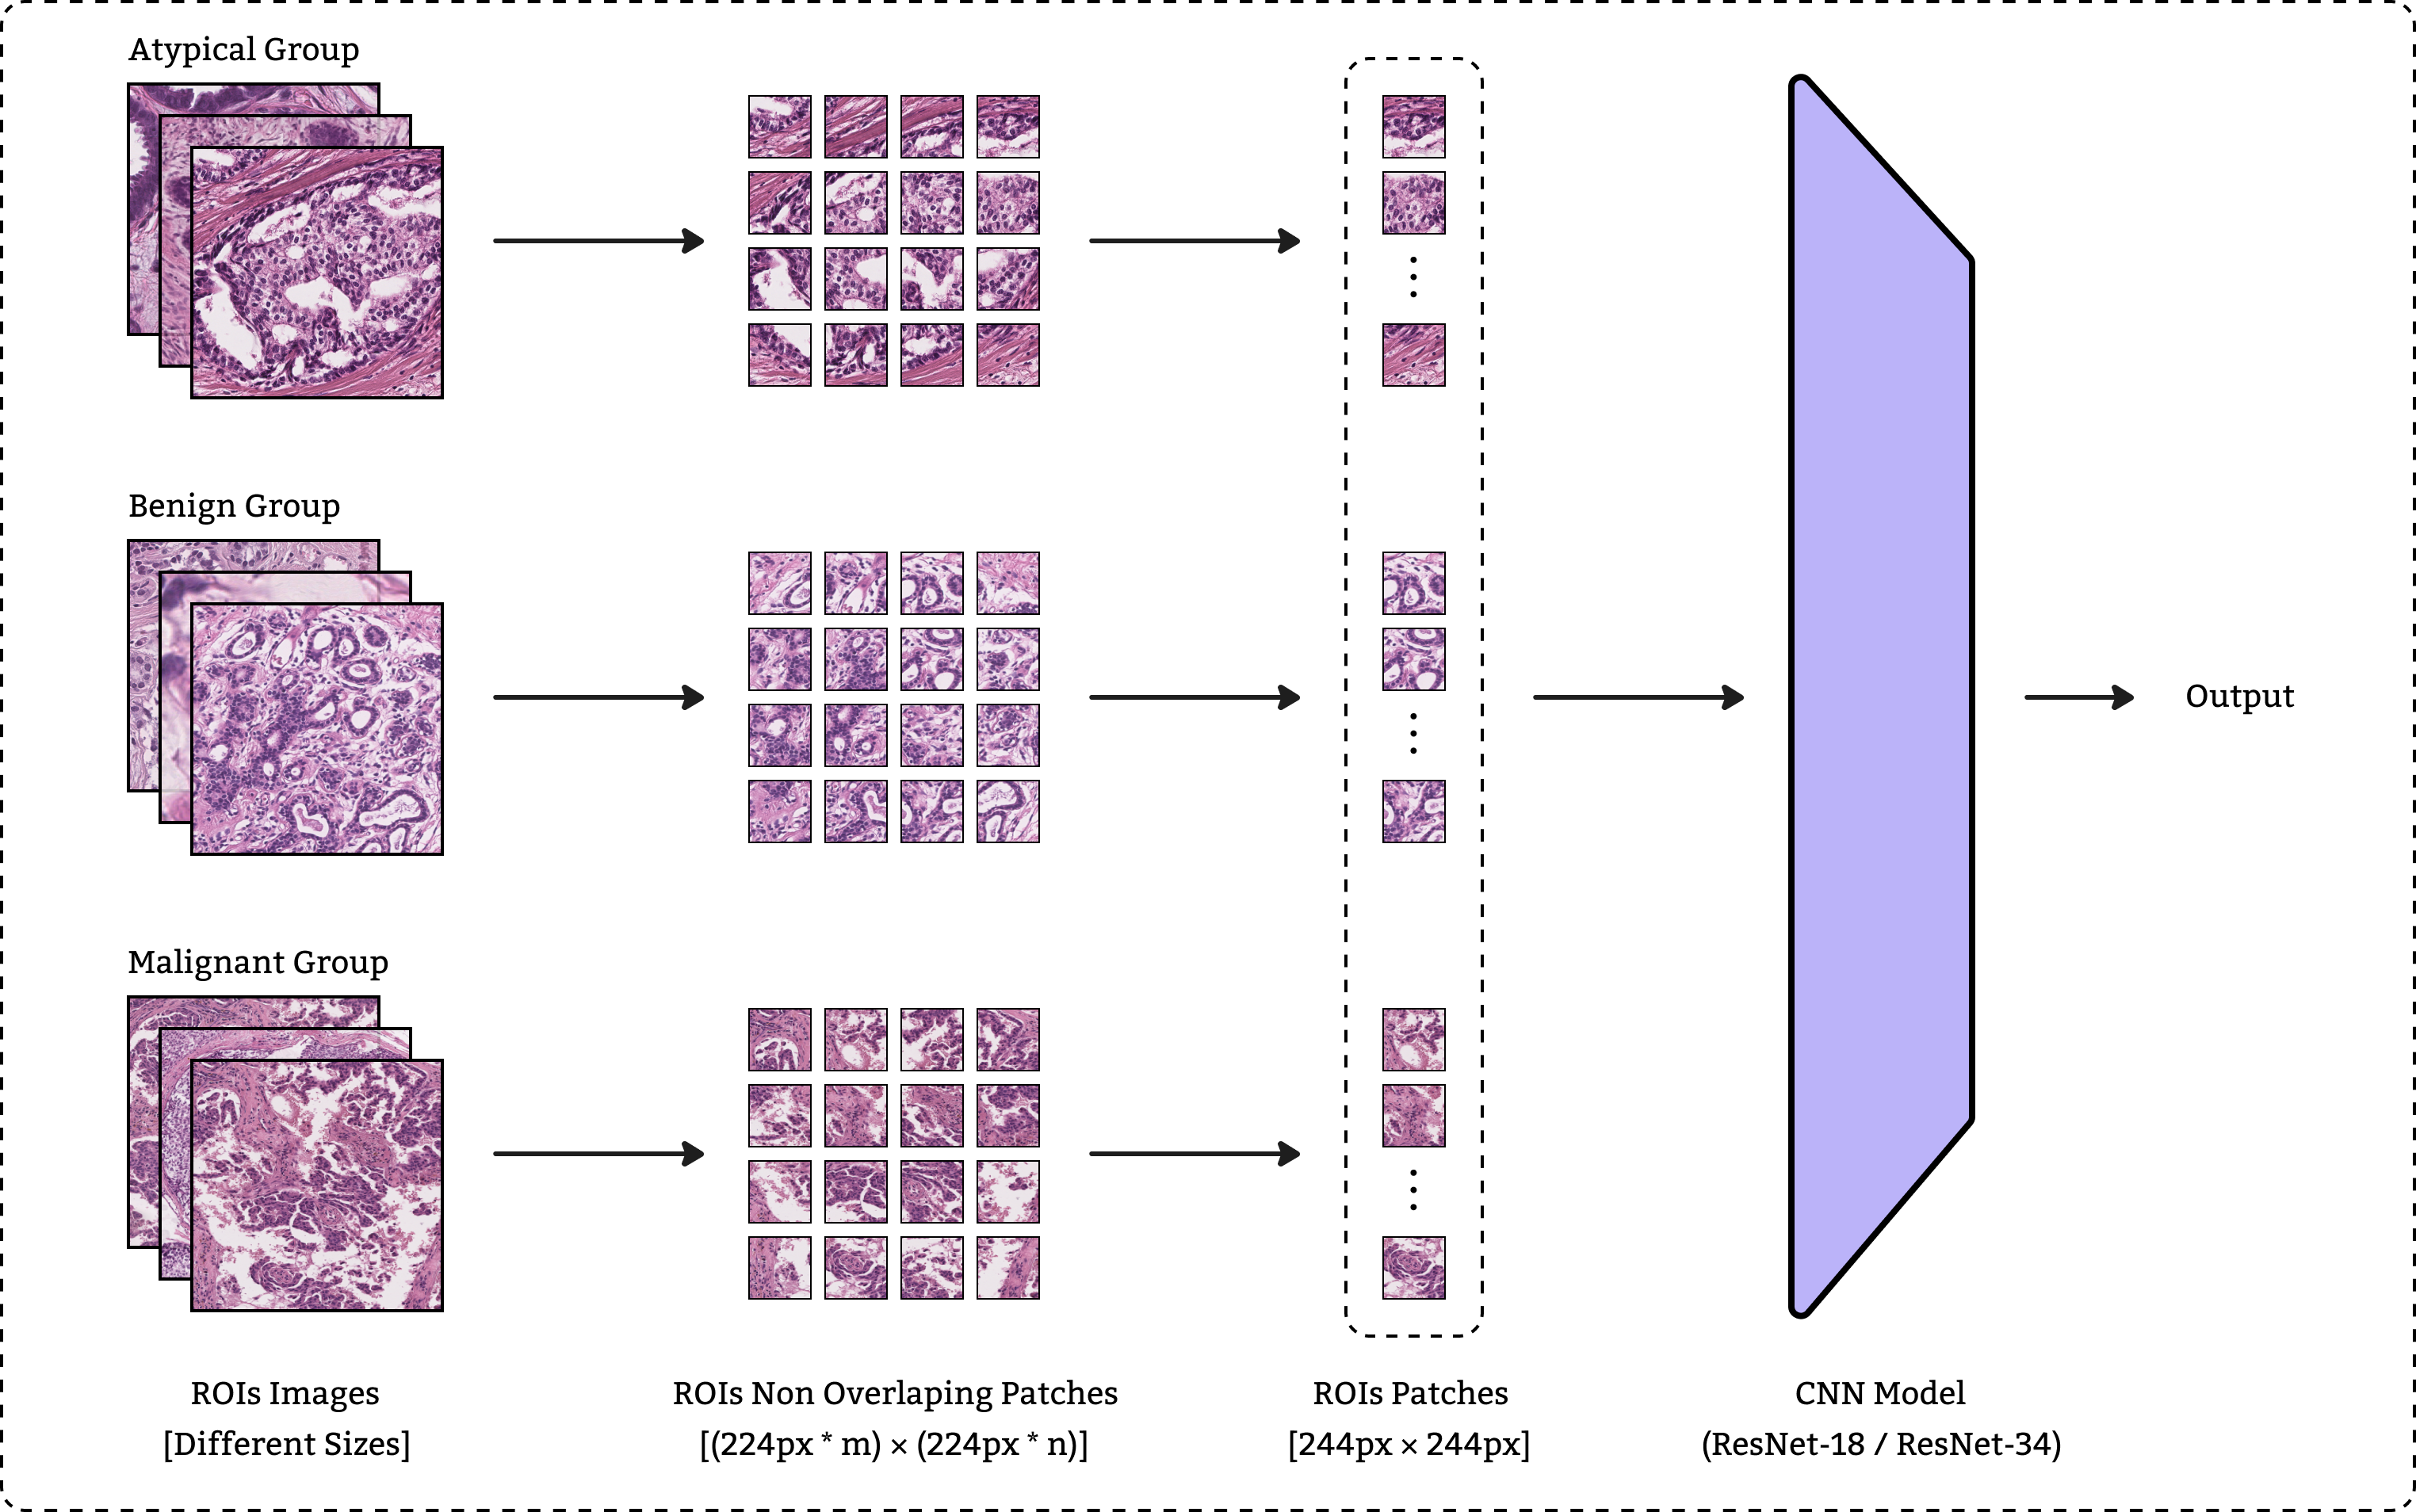
\includegraphics[width=\textwidth]{figures/fine-tuning/fine_tuning.png}
    \caption{Fine-tuning process on \acrshort{BRACS}' \acrshort{ROI} images.}
    \label{fig:fine_tuning}
\end{figure}

% \subsubsection{ROIs Preprocessing}

\noindent Before fine-tuning the models on \acrshort{ROI} images some preprocessing must be made so they can be fed to the \acrshort{ResNet} models which require an input of 224 x 224 pixels. However, The \acrshort{ROI}s in the dataset have varying dimensions, i.e they can not be divided into equal patches, which poses a challenge for direct input of our models. To address this issue, we had to choose one of two options:
\begin{itemize}
    \item Using overlapping 224 x 224 pixels patches to cover the whole image.
    \item Resizing the height and width to the closest multiple of 224 (could be bigger or smaller than the current value).
\end{itemize}
\noindent We opted for the latter because the first option could produce too many patches, which would drastically elevate the training time. By resizing each image to the closest multiple of 224, we ensured compatibility with the image patching process, allowing the resized image to be covered entirely by 224 x 224 pixel patches.\\

\noindent After resizing, we employed an image patching algorithm, splitting each \acrshort{ROI}s image into multiple non-overlapping patches of size 224 x 224 pixels, while attributing the label of the original image to the label of the patch (weak patch labeling) and keeping the same original train, validation and test splits they belonged to originally. Furthermore we ensured that the resizing process does not cause any loss of information in the original image,Tables \autoref{tab:splits_distribution} and \autoref{tab:category_distribution} reports the distribution of the patches according to their types and sub-types.

% \subsubsection{Patches Dataset}

\begin{table}[ht]
    \centering
    \small
    \begin{adjustbox}{max width=\textwidth} % scale the table to fit within text width
        \begin{tabular}{@{}l|rrrr}
            \toprule
            Data & Benign & Atypical & Malignant & Total \\
            \midrule
            Train & 141578 & 33898 & 157798 & 333274  \\
            Validation & 8151 & 4472 & 18635 & 31258 \\
            Test & 13137 & 6191 & 20564 & 39892 \\
            \midrule
            Total & 162866 & 44561 & 196997 & \textbf{404424}\\
            \bottomrule
        \end{tabular}
    \end{adjustbox}
    \caption{Data distribution of patches count across different splits and lesion types.}
    \label{tab:splits_distribution}
\end{table}

\begin{table}[ht]
    \centering
    \small
    \begin{adjustbox}{max width=\textwidth} % scale the table to fit within text width
        \begin{tabular}{@{}l|rrrrrrrr}
            \toprule
            Split & \acrshort{N} & \acrshort{PB} & \acrshort{UDH} & \acrshort{FEA} & \acrshort{ADH} & \acrshort{DCIS} & \acrshort{IC} & Total \\
            \midrule
            Train & 27470 & 94454 & 19654 & 16821 & 17077 & 68491 & 89307 & 333274 \\
            Validation & 3267 & 3018 & 1866 & 2793 & 1679 & 5986 & 12649 & 31258 \\
            Test & 3501 & 5509 & 4127 & 2499 & 3692 & 5303 & 15261 & 39892 \\
            \midrule
            Total & 34238 & 102981 & 25647 & 22113 & 22448 & 79780 & 117217 & \textbf{404424} \\
            \bottomrule
        \end{tabular}
    \end{adjustbox}
    \caption{Data distribution of patches count across different splits and categories.}
    \label{tab:category_distribution}
\end{table}

\newpage
\noindent A comparison between \autoref{tab:splits_distrib} and \autoref{tab:splits_distribution} shows that Malignant became the predominant class, and that is due to the fact that type IC has the ROIs with the highest resolution across the dataset, which means it produces more patches (\autoref{tab:category_distribution}).

\subsection{Feature Extraction}

\subsubsection{Grid-based feature extraction}
The goal of the Grid-based Feature Extraction stage (\acrshort{GFE}) is to create a more compact representation of the original image that can be processed by the Attention-based Classifier. To achieve this goal, the \acrshort{GFE} takes as an input the original gigapixel Whole Slide Image (\acrshort{WSI}) and transforms it into a lower dimensional feature space while preserving local spatial relationships.\\
The \acrshort{WSI} is partitioned into a set of non overlapping patches. These patches are then mapped into feature vectors by applying deep learning models, such as Convolutional Neural Networks (\acrshort{CNN}s) and Vision Transformers (\acrshort{ViT}s). The resulted feature vectors are rearranged in a grid format to maintain the spatial proximity information of the original patches in the \acrshort{WSI}.  \autoref{fig:gfe_stage} shows an illustrated representation of the \acrshort{GFE} stage.

\begin{figure}[H]
    \centering
    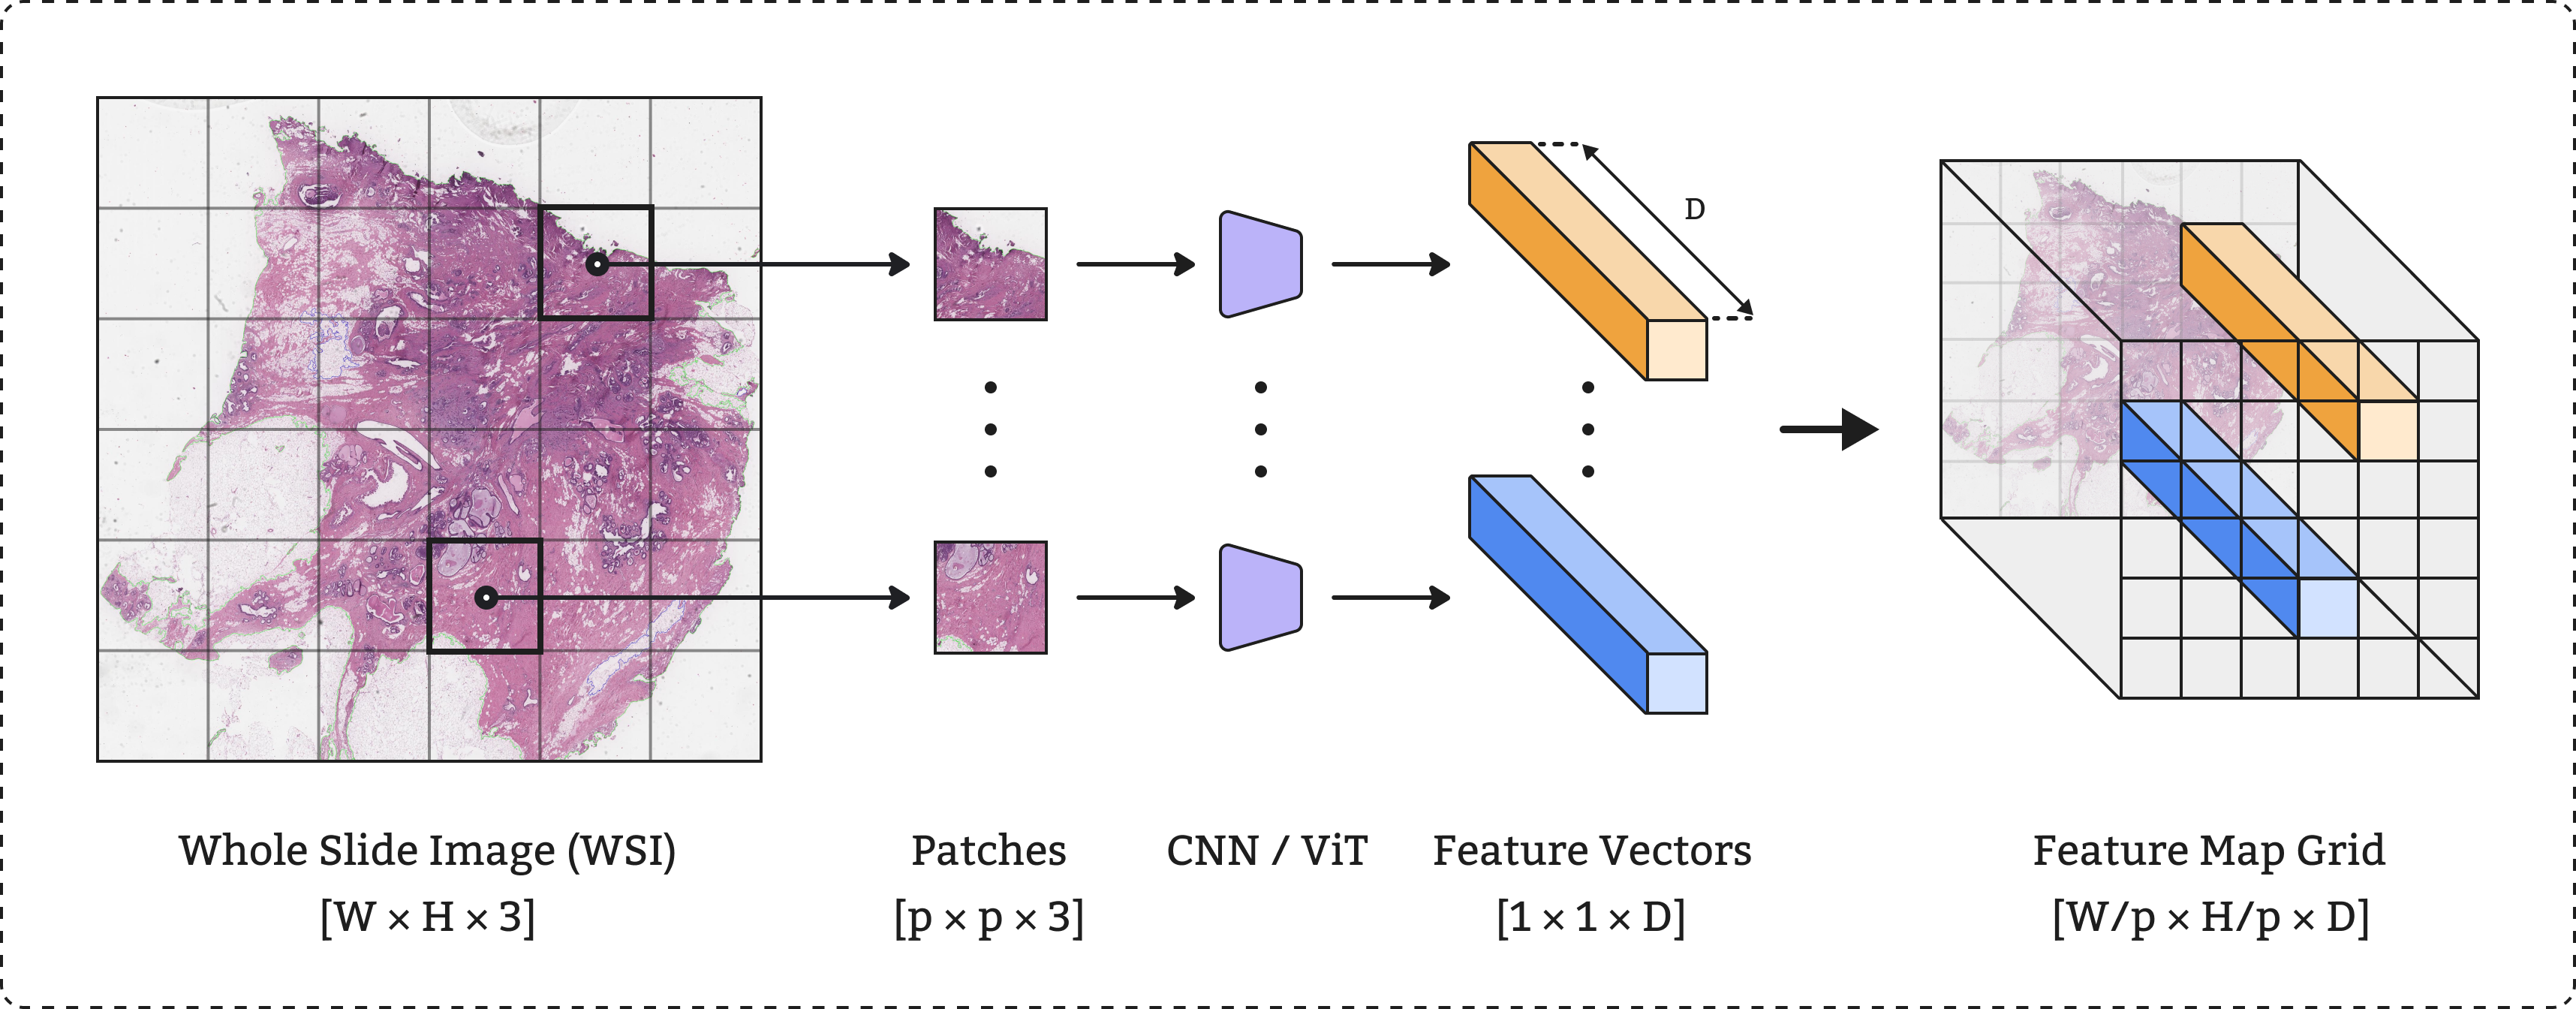
\includegraphics[width=\textwidth]{figures/ABNN_methods/GFE.png}
    \caption{Grid-Based Feature Extraction (\acrshort{GFE}) $^{\text{\cite{Gigapixel}}}$.}
    \label{fig:gfe_stage}
\end{figure}

\noindent For more details, let’s $W \in R^{W \times H \times 3}$ represents the input image, where $W$ and $H$ are the width and the height of the Whole Slide Image with three color channels (RGB). The \acrshort{GFE} divides the input image into a set of non-overlapping patches $X = \{x_{i,j}\}$, and that can be done by sampling $W$ along the $i\textsuperscript{th}$ row and $j\textsuperscript{th}$ column according to a uniform grid of size $p \times p \times 3$. Each of these patches is then independently fed to a \acrshort{CNN} or a \acrshort{ViT}, which maps it into a $1 \times 1 \times D$ feature vector obtained from the network's global average pooling layer. These patch-wise feature vectors are then assembled into a three-dimensional compressed representation organized in a grid $G \in R^{W’ \times H’ \times D}$ where $W' = \frac{W}{p}$ and $H' = \frac{H}{p}$, so that the spatial arrangement of the vectors in G corresponds to the original positioning of their respective patches in the \acrshort{WSI}.

\subsubsection{Feature extraction with patch selection}

\noindent Contrary to grid based feature extraction which takes as input the entire \acrshort{WSI} image, in this method the \acrshort{WSI} first goes through \acrshort{CLAM} for patch selection before doing any feature extraction. \acrshort{CLAM} (Clustering-constrained Attention Multiple instance learning) is a method proposed in \cite{CLAM}. It is a high-throughput and interpretable method for data efficient \acrshort{WSI} classification using slide-level labels without any \acrshort{ROI} extraction or patch-level annotations, and is capable of handling multi-class subtyping problems. One of its main functionalities is segmentation and patching, in the context of feature extraction with patch selection it is used as a pre-processing step to locate tissue regions in each \acrshort{WSI}, i.e removing the background. \acrshort{CLAM} returns equal patches coordinates for a given \acrshort{WSI} ( see \autoref{fig:clam}), these coordinates are then used to select which patches to be fed to the feature extraction model (\acrshort{ResNet}-18, \acrshort{ResNet}-34 or a ViT-S/16), each patch produces a feature vector, the vectors are then assembled to produce a compact representation of the \acrshort{WSI} and finally saved to the disk as tensors. \autoref{fig:fe} shows a schematic representation of the overall process.

\begin{figure}[H]
    \centering
    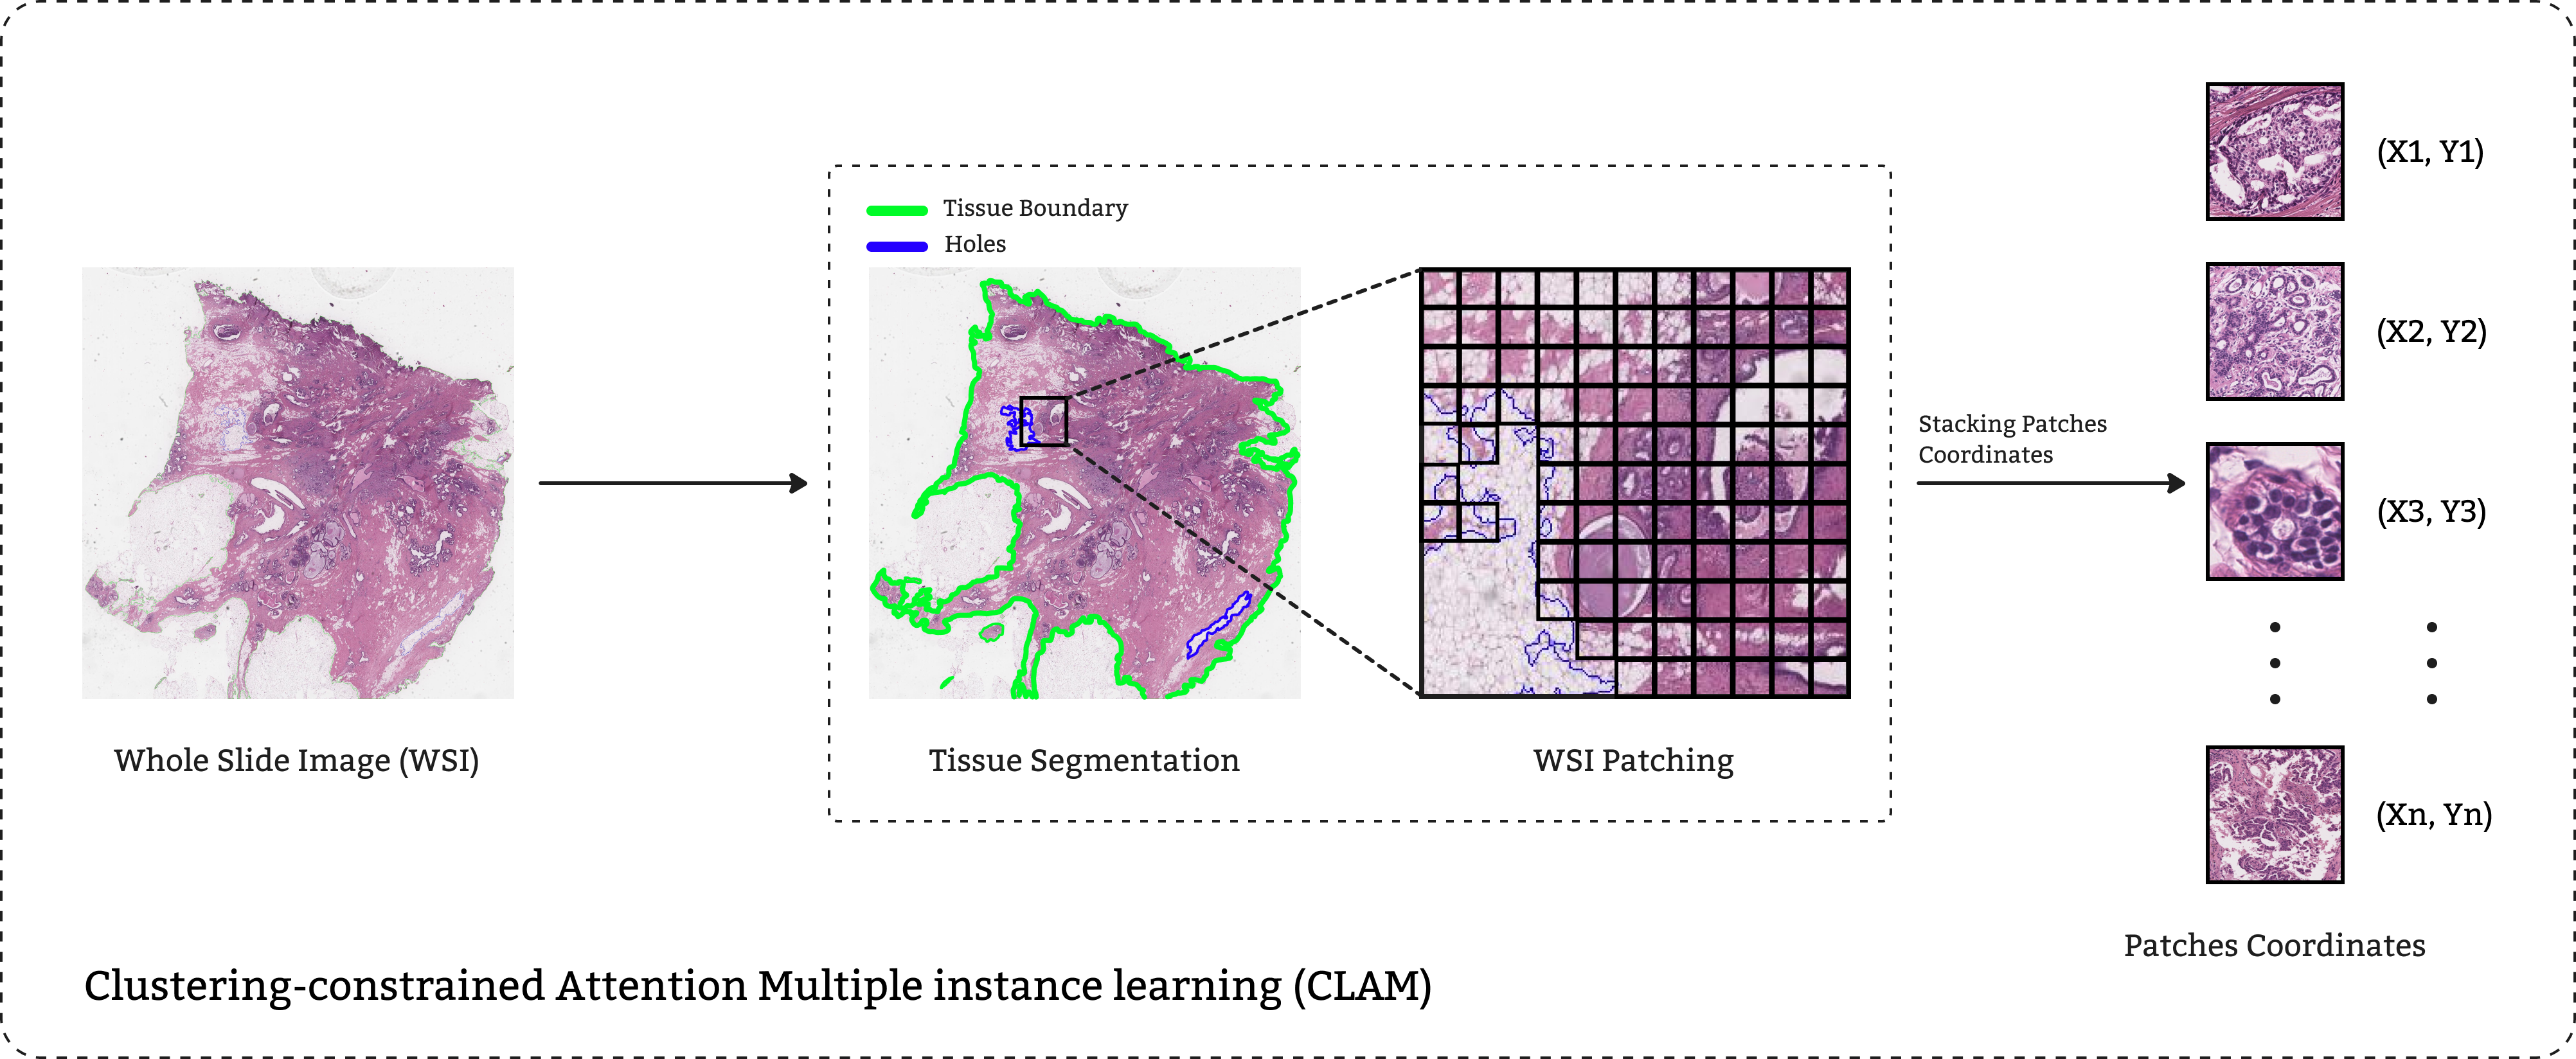
\includegraphics[width=\textwidth]{figures/ACMIL_methods/clam.png}
    \caption{Clustering-constrained Attention Multiple instance learning}
    \label{fig:clam}
\end{figure}

\begin{figure}[H]
    \centering
    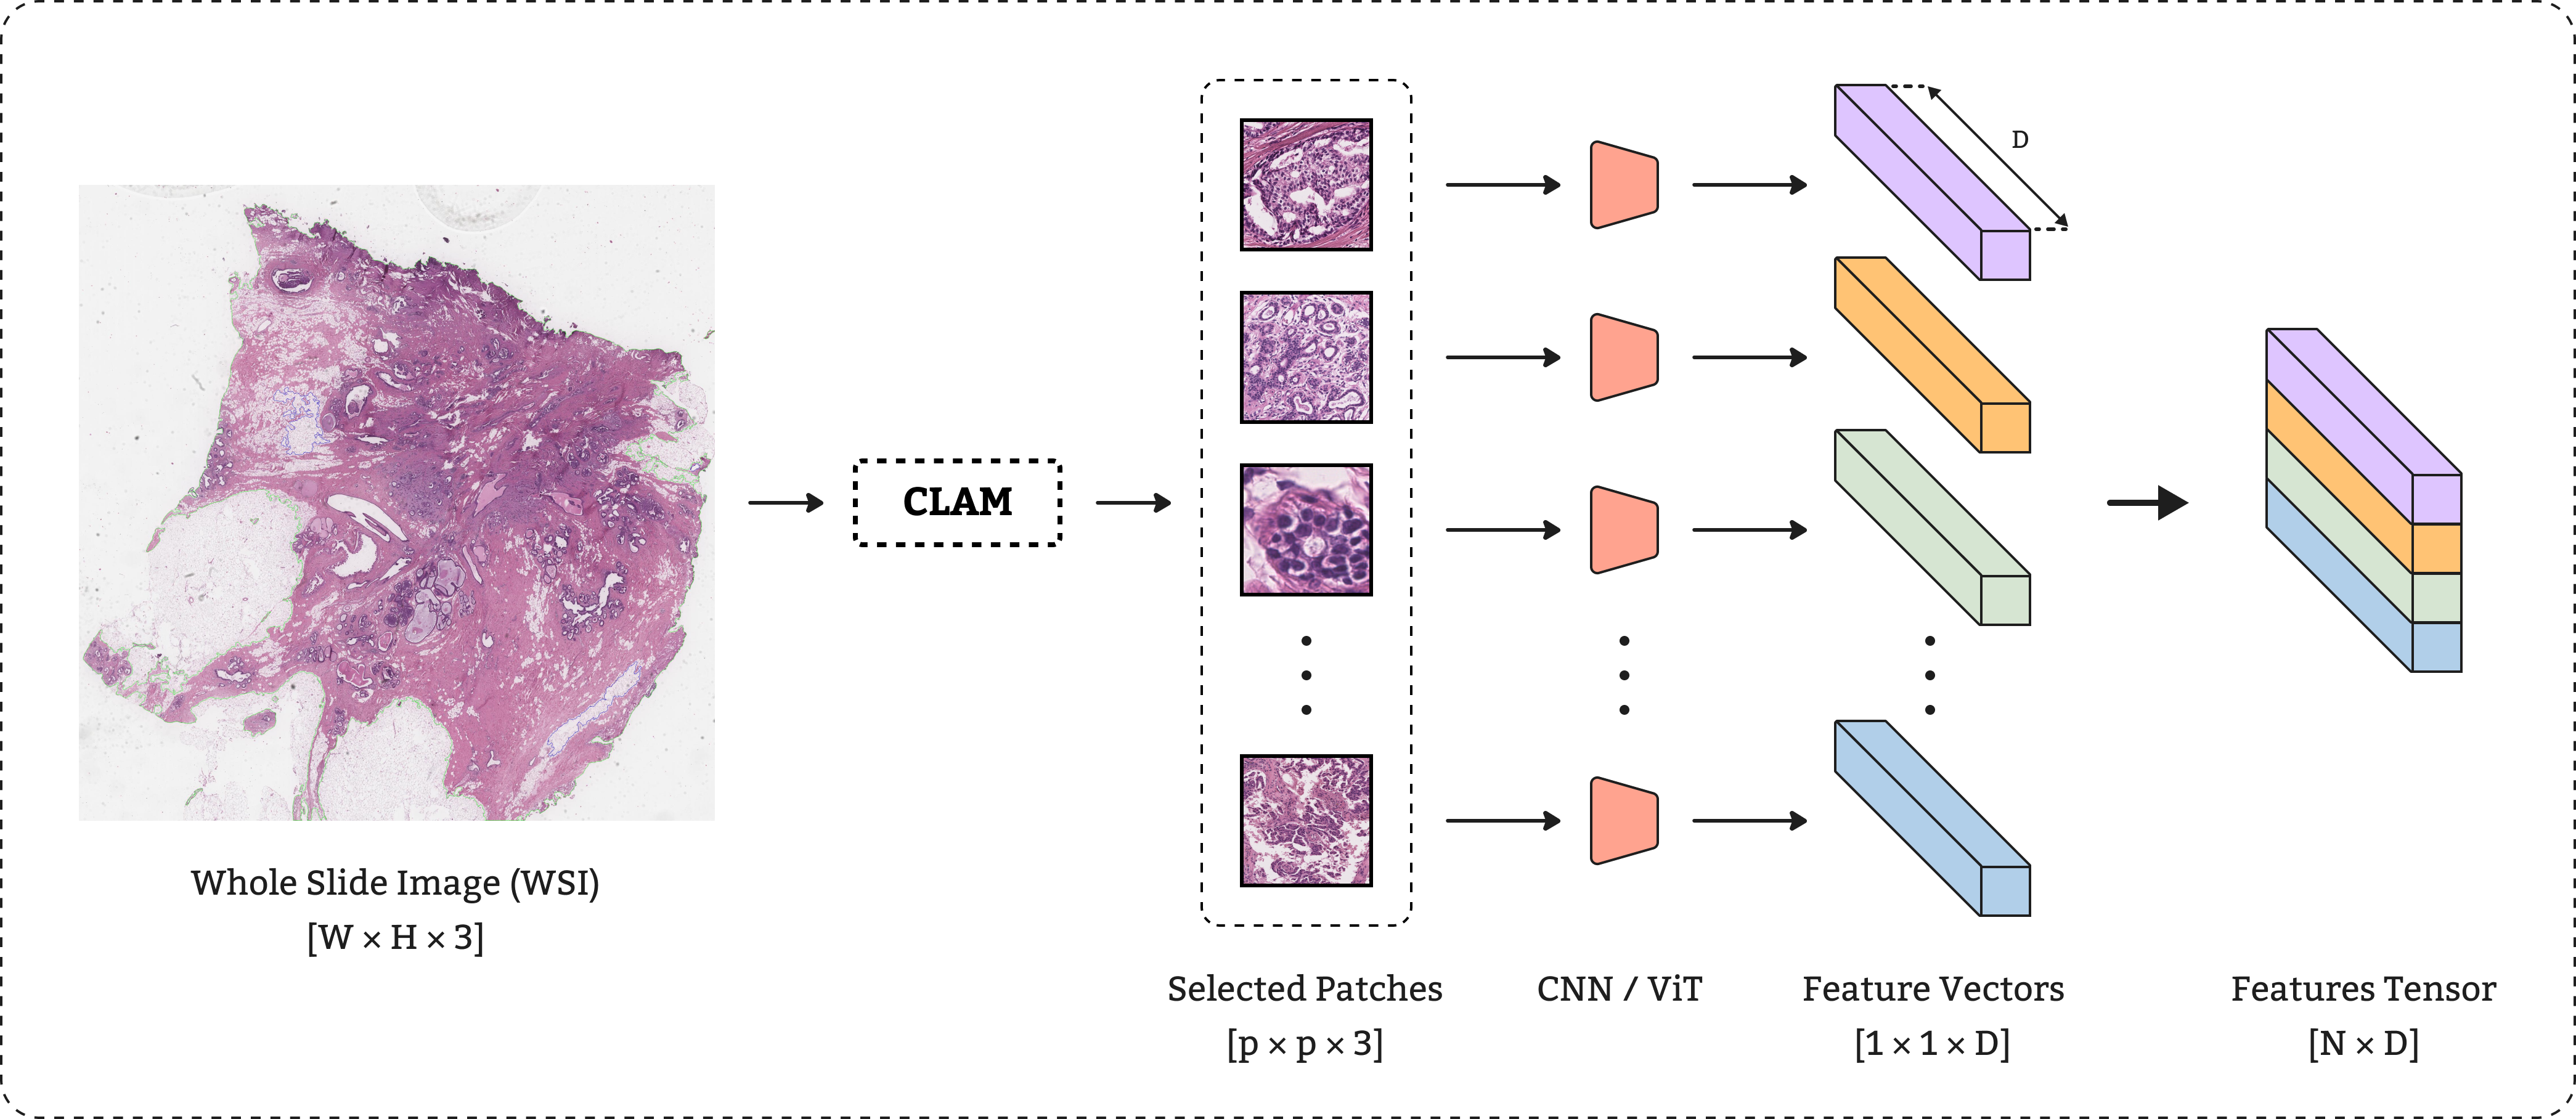
\includegraphics[width=\textwidth]{figures/ACMIL_methods/FE.png}
    \caption{Feature extraction with patch selection}
    \label{fig:fe}
\end{figure}



\subsection{\acrshort{WSI} Classifiers}

\subsubsection{Min-Max attention based classifier}
\noindent Min-Max attention based classifier (\acrshort{MMABC})$^\text{\cite{Gigapixel}}$ is architecture taht exploits 3D convolutional layers and min-max attention mechanisms to extract relevant patterns from the compressed \acrshort{WSI},without ignoring the relative location between the patches' embeddings.\\

\noindent the model operates on the outputs of grid-based feature extraction technique (\acrshort{GFE}) which means it receives an input $G \in R^{W' \times H' \times D}$,where $W'$ and $H'$ are the width and the height of the compressed \acrshort{WSI} and relies on a 3D convolutional layer for feature extraction then those features are fed to two different attention layers (min \& max attention layers) and the generated feature vectors from both layers are concatenated then passed to a softmax layer to output the probabilities. \autoref{fig:ac_stage} shows a schematic representation of the proposed attention
network.\\

\begin{figure}[H]
    \centering
    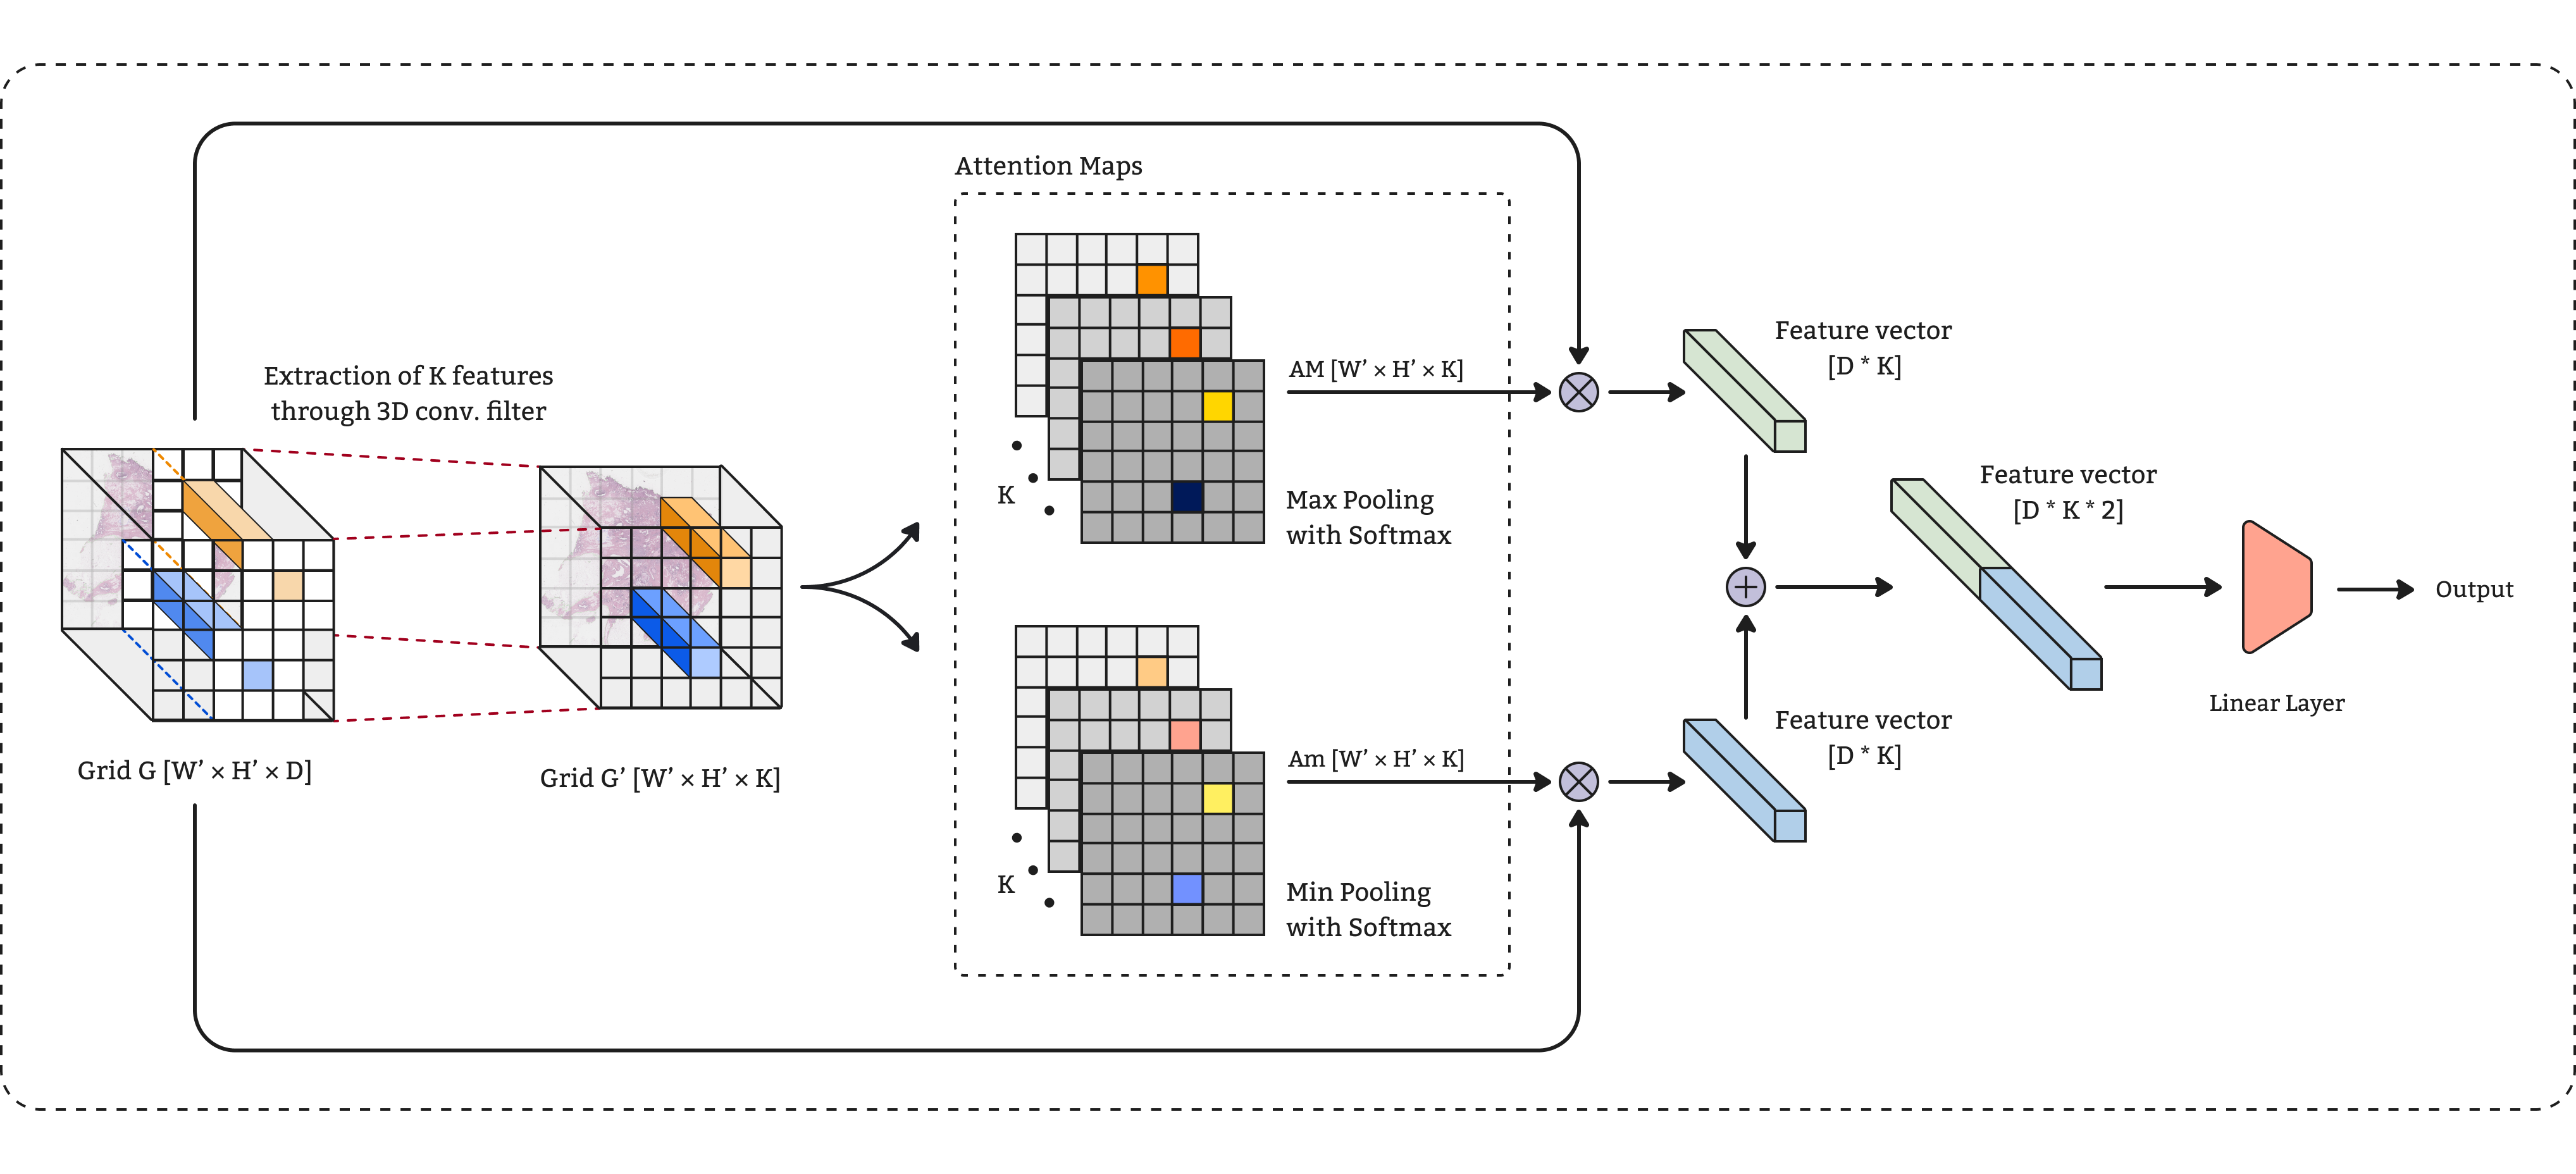
\includegraphics[width=\textwidth]{figures/ABNN_methods/AC.png}
    \caption{Min-Max attention based classifier (\acrshort{AC}) $^{\text{\cite{Gigapixel}}}$.}
    \label{fig:ac_stage}
\end{figure}

\noindent Processing the compressed WSI with a 3D convolutional layer involves using a 3D convolutional layer to extract $K$ filters from $G$, resulting in a tensor $G' \in \mathbb{R}^{W' \times H' \times K}$. The idea behind this is to extract features based on the relative location between patches, as each patch was treated independently during the GFE. The min attention mechanism divides each filter of the input features $G'$ into smaller non-overlapping regions of dimensions $S \times S$, then only the minimum value from each region is kept while the others are set to zero. The softmax function is applied to the flattened output of the previous stage, which results in $K$ attention maps $A_{\text{min}} \in \mathbb{R}^{W' \times H' \times K}$.\\

\noindent The max attention operates similarly, but instead, only the maximum value from each region is kept, outputting $M$ attention maps $A_{\text{max}} \in \mathbb{R}^{W' \times H' \times K}$. Finally, the attention maps of each attention layer independently are multiplied with each channel of the original input to result in two feature vectors, each of dimension $D \times K$, one corresponding to the min-layer and the other to the max-layer. The two feature vectors are then concatenated to get a feature vector of dimension equal to $D \times K \times 2$. The feature vector outputted by the min-max attention mechanism is fed to a linear layer with a softmax activation function to generate the probabilities of each class.


\iffalse
\subpar{Processing the compresses WSI with 3D convolutional layer}

\noindent A 3D convolutional layer is used to extract $K$ filters from $G$ resulting in a tensor $G' \in R^{W' \times H' \times K}$,The idea behind this is to extract features based on the relative location between patches as each patch was treated independently during the \acrshort{GFE}.
\subpar{Min \& Max attention mechanisms}
\noindent The min attention mechanism divides each filter of the input features $G'$ into smaller non-overlapping regions of dimensions $S \times S$ then only the minmum value from each region is kept while the others are set to zero,then the softmax function is applied on the flattened output of the previous stage, which results in $K$ attention maps $A_{min} \in R^{W' \times H' \times K}$.\\

\noindent The max attention operates similarly,but instead only the maximum value from each region is kept, outputting M attention maps $A_{max} \in R^{W' \times H' \times K}$.\\

\noindent finally attention maps of each attention layer independently, are multiplied with each channel of the original input to result in two feature vectors each of dimension $D * K$,one corresponds to the min-layer and the other to the max-layer, the two feature vectors are then concatenated to get a feature vector of dimension equals to $D * K * 2$.
\subpar{Softmax Layer}
\noindent The feature vector outputed by the min-max attention mechanism is fed to a linear layer with softmax activation function to generate the probabilities of each class.
\fi

\subsubsection{Attention-Challenging Multiple Instance Learning}

\noindent Attention-Challenging Multiple Instance Learning $^{\text{\cite{ACMIL}}}$ (\acrshort{ACMIL} : \autoref{fig:acmil-schema}) is an attention-based architecture that was proved successful in reducing the overfitting for various cancer datasets including \acrshort{BRACS} Dataset, by introducing a new regularization technique called \acrshort{STKIM}(Stochastic Top-K Instance Masking),as well as a new loss function that insures the diversity of the extracted features.\\

\noindent The \acrshort{ACMIL} model operates on an input $x \in R^{N \times D}$ representing the embeddings of flattened patches, where $N$ is the number of patches and $D$ is the embedding's dimension.

\begin{figure}[H]
    \centering
    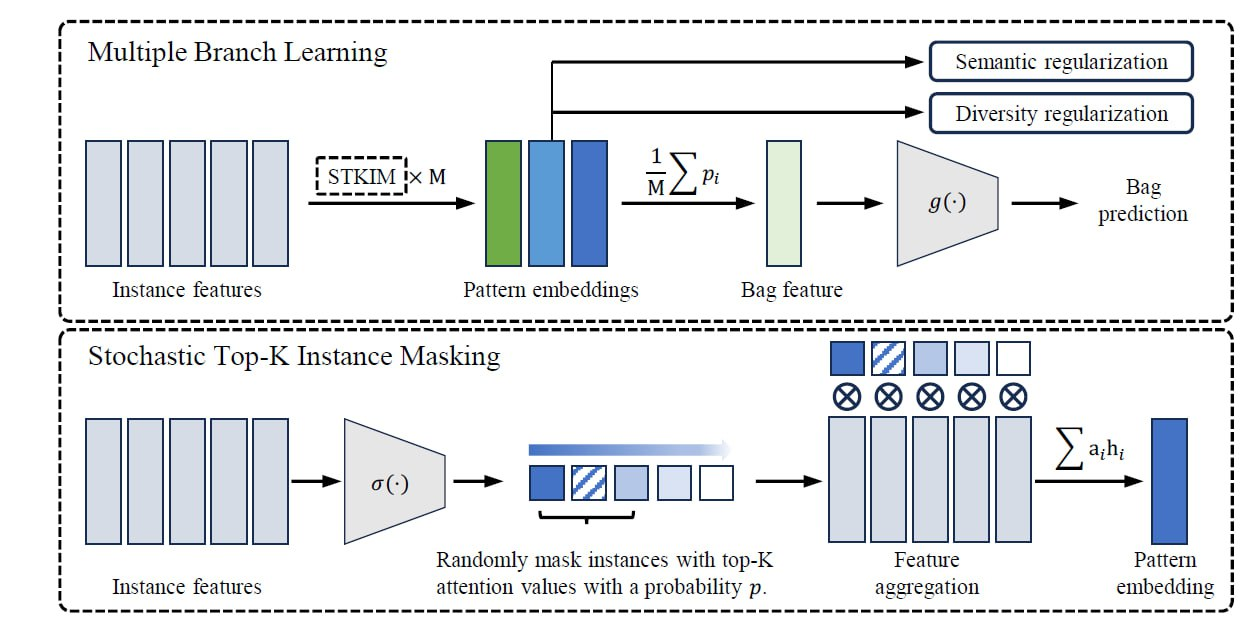
\includegraphics[width=\textwidth]{figures/ABNN_methods/acmil.jpg}
    \caption{An Overiew of the \acrshort{ACMIL} Architecture$^{\text{\cite{ACMIL}}}$.}
    \label{fig:acmil-schema}
\end{figure}

% \subpar{Dimentiality Reduction Layer}

\newpage
\noindent First of all the input (a compressed WSI) is past to a dimentiality reduction layer is a regular \acrshort{MLP} network that maps the dimension of the input patches features of dimension $D$ to a lower dimenion $D'$.

$$
X' = DimReduction(X)
$$

\noindent The the output $X'$ is then processed by the multi-branch attention block,to better understand the multi-branch attention mechanism we first need to understand the attention gated mechanism,The attention gated mechanism allows the model to focus on different parts of the of the input by computing a score for each patch embedding.\\

\noindent An attention gated layer is composed of three matrices $U \in R^{D' \times D_{hidden}}$,$V \in R^{D' \times D_{hidden}} $ and $W \in R^{D_{hidden} \times 1}$ : 

\begin{itemize}
    \item the matrix $U$ reduces the dimension of the input tensor to $D_{hidden}$ followed by a $tanh$ activation function resulting in matrix $U_{output} \in R^{N \times D_{hidden}}$.
    \item the matrix $V$ is used in conjunction with the $sigmoid$ function to control the flow of the information in the network by computing values between 0 and 1, resulting in matrix $V_{output} \in R^{N \times D_{hidden}}$.
    \item the matrices $V_{output}$ and $U_{output}$ are multiplied element wise.
    \item finally the matrix $W$ followed by a transpose operation then the $softmax$ function is used to compute a score for each patch, resulting in an attention filter of dimenions $A \in R^{1 \times N}$.
\end{itemize}

$$
\begin{cases}
a = ((tanh(X' \times U) * sigmoid(X' \times V)) \times W)^T\\
A = softmax(a)
\end{cases}
$$

% \noindent \underline{Multi-branch attention} : \\

\noindent The multi-Branch attention modifies the attention gated mechansim by not only computing one score per patch but multiple ones,this can be acheived by modifying the dimensions of the matrix $W$ to be $D_{hidden} \times K$,where $K$ is the number of branches,resulting in  attention filter $A \in R^{K \times N}$,which can be seen as having multiple branches (Gated Attention layers) that process the input simultaneously.

\subpar{Stochastic top-k instance masking}

\noindent Stochastic top-k instance masking (\acrshort{STKIM}) is a regularization technique similar to dropout that randomly masks (sets to zero) the top-k attention scores with probability of p, this technique deals with one of the main reasons of overfitting in whole slide images,which is the model relying on small number of patches in the decision making by randomly masking a portion of the patches with the higher scores,we encourage the model to extract patterns from the other patches.\\

\noindent \acrshort{STKIM} is applied an the outputs of the attention layer before applying the softmax function to ensure that scores always add up to one, and just like dropout \acrshort{STKIM} is deactivated in inference mode.

\newpage
\subpar{The loss function}

\noindent To insure that the model is extracting meaningfull and diverse patterns from the training data a new loss function had to be introduced,it is composed of three sub-losses : \\

% \begin{itemize}

\noindent \underline{Diversity Loss} : \\

\noindent To ensure that the branches are not learning similar patterns a diversity loss is introduced,it is simply the average cosine similarity between the vectors representing the attention scores (before applying the softmax function) given to the patches by each \\ branch :

$$
L_{d} = \frac{2}{K * (K - 1)} \sum\limits_{i=1}^{K} \sum\limits_{j=i+1}^{K} cos(a_{i},a_{j})
$$

\noindent \underline{Semantic Loss} : \\

\noindent Diversity loss alone is not very usefull as the model can learn diverse but non-relevant patterns,so a semantic loss is added,by calculating the outputs of the model based on the attention scores of each branch separately,then calculating the average cross entropy loss based on those outputs and the true labels,this requires an \acrshort{MLP} for each branch :

$$
\begin{cases}
    L_{s} = - \frac{1}{K} \sum\limits_{i=1}^{M} Y log(\hat{Y_{i}}) + (1 - Y) log(1 - \hat{Y_{i}})\\
    \hat{Y_{i}} = softmax(MLP_{i}(A_{i} \times X'))
\end{cases}
$$

\noindent \underline{The bag classifier's loss function} : \\

\noindent For the final prediction is made by calculating the attention values for each branch are averaged,multiplied by the input matrix then fed to an \acrshort{MLP} network to generate the output,these quality of the prediction are assessed using the regular cross entropy loss :

$$
\begin{cases}
L_{b} = - (Y log(\hat{Y}) + (1 - Y) log(1 - \hat{Y})) \\
\hat{A} = \frac{1}{K} \sum\limits_{i=1}^{K} A_{i}\\
\hat{Y} = softmax(MLP(\hat{A} \times X'))
\end{cases}
$$

% \end{itemize}

\noindent \\The overall loss function is simply the sum of the three losses :

$$
L = L_{s} + L_{d} + L_{b}
$$

\subsubsection{Hierarchical Image Pyramid Transformers}

\noindent Hierarchical Image Pyramid Transformers (\acrshort{HIPT}) is a Vision Transformer (\acrshort{ViT}) architecture that was proposed in \cite{HIPT}, designed for analyzing gigapixel whole-slide images (\acrshort{WSI}s) in computational pathology. \acrshort{HIPT} leverages the inherent hierarchical structure of \acrshort{WSI}s to learn high-resolution image representations through self-supervised learning. Pretrained on a large dataset covering 33 cancer types and evaluated across multiple slide-level tasks, \acrshort{HIPT} demonstrates superior performance in cancer subtyping and survival prediction. Adapting the \acrshort{HIPT} architecture to the \acrshort{BRACS} Dataset is a novel experimentation which has not been done before. \\
\begin{figure}[H]
    \centering
    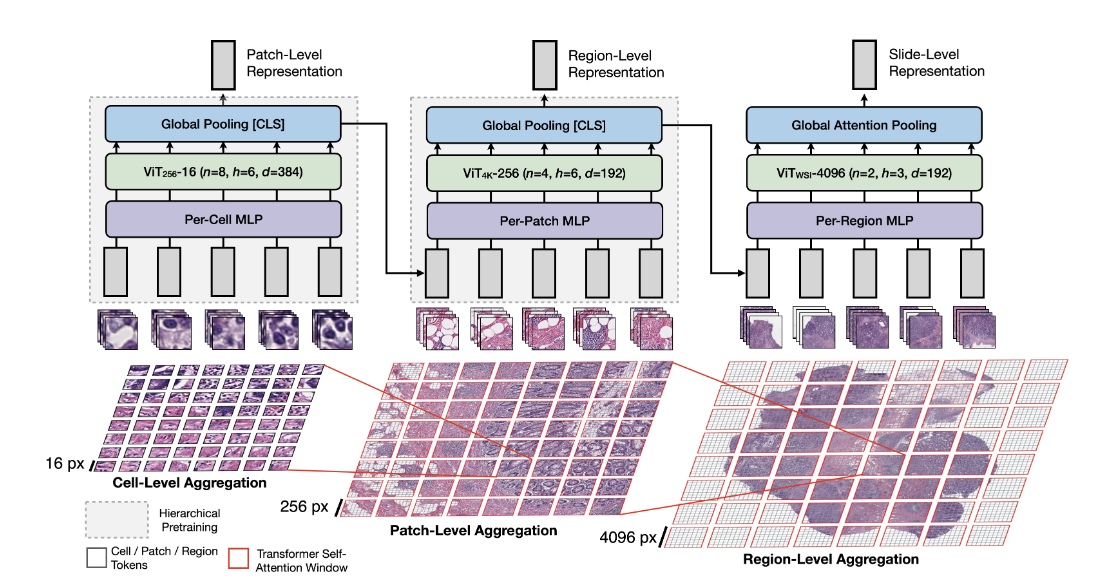
\includegraphics[width=1\linewidth]{figures/hipt.png}
    \caption{HIPT Architecture $^{\text{\cite{HIPT}}}$.}
    \label{fig:hipt}
\end{figure}
\noindent As depicted in \autoref{fig:hipt}, \acrshort{HIPT} uses a hierarchical structure to process \acrshort{WSI}s through multiple scales of visual tokens, systematically aggregating information from smaller patches to larger regions and finally to the entire slide. This hierarchical processing is crucial for capturing the complex and multi-scale patterns present in pathology images, we distinguish four different levels : \\

% \subpar{Hierarchical Levels}
% \begin{itemize}
    \noindent \textbf{Cell-Level (16×16 pixels):} 
    16×16 pixel patches are tokenized and processed using a Vision Transformer (ViT256-16) to learn fine-grained detailed cell-level representations.\\
    
    \noindent \textbf{Patch-Level (256×256 pixels):} 
    Tokens representing 256×256 pixel patches are further aggregated using another Vision Transformer (ViT4096-256), capturing interactions within a larger local clusters of cell interactions.\\
    
    \noindent \textbf{Region-Level (4096×4096 pixels):} 
    Tokens for 4096×4096 pixel regions are aggregated using a final Vision Transformer (ViTWSI-4096), forming a macro-scale representation of the \acrshort{WSI}.\\
    
    \noindent \textbf{Slide-Level:} The aggregated tokens from the region-level are combined to integrate information from all hierarchical levels and provide a comprehensive representation of the entire \acrshort{WSI}.\\
% \end{itemize}

% \subpar{Self-Supervised Learning}

\iffalse
\noindent \acrshort{HIPT} employs self-supervised learning, specifically using a technique called student-teacher knowledge distillation (\acrshort{DINO}) \cite{DINO}, to pretrain each hierarchical level. \\
\paragraph{Student-Teacher Framework:}
Two networks (student and teacher) are trained simultaneously. The teacher network, updated more slowly using an exponential moving average of the student's parameters, stabilizes the learning process.
\paragraph{Multi-View Learning:}
Different augmented views of the same image are used. The student network processes these views to produce embeddings that are aligned with those of the teacher network, encouraging invariant feature learning.
\paragraph{Self-Distillation Loss:}
The student’s embeddings are matched to the teacher’s embeddings, ensuring the model learns robust and generalizable features.
\fi

\noindent \acrshort{HIPT} employs self-supervised learning, specifically using a technique called student-teacher knowledge distillation (\acrshort{DINO}) \cite{DINO}, to pretrain each hierarchical level. In the student-teacher framework, two networks (student and teacher) are trained simultaneously. The teacher network, updated more slowly using an exponential moving average of the student's parameters, stabilizes the learning process. Multi-view learning is employed where different augmented views of the same image are used, and the student network processes these views to produce embeddings that are aligned with those of the teacher network, encouraging invariant feature learning. The self-distillation loss matches the student’s embeddings to the teacher’s embeddings, ensuring the model learns robust and generalizable features.\\

% \subpar{Hierarchical Pretraining}

\noindent \acrshort{HIPT} involves two main stages of pretraining, each focusing on different scales of the input data to capture both fine-grained and coarse-grained morphological features essential for diagnostic tasks,In this stage, 256 × 256 pixel patches of histology images are used for pretraining a Vision Transformer (ViT256-16). This process employs the \acrshort{DINO} framework, which includes a student network and a teacher network. The student network is trained to match the probability distribution output of the teacher network using a cross-entropy loss function. Data augmentation plays a critical role here, with the introduction of local views (96 × 96 crops) and global views (224 × 224 crops) to encourage the model to learn local-to-global correspondences. This approach helps the model capture detailed cellular structures and their interactions within the local tissue environment, which are crucial for understanding cellular morphology in pathology, The second stage involves a more extensive scale, using 4096 × 4096 pixel regions. Here, the pretrained ViT256-16 model is reused to tokenize these larger regions into sequences of 256 tokens. These tokens are then used as input to another Vision Transformer model (ViT4096-256) for further pretraining. This stage also follows a similar \acrshort{DINO} framework, with data augmentations adjusted to match the scale of the larger patches, such as local-global crops of 6 × 6 and 14 × 14. This stage is crucial for capturing broader spatial organizations and macro-scale interactions within the tissue, such as tumor invasion patterns and lymphocytic infiltration, which are significant for understanding the overall tissue architecture and for making accurate diagnostic and prognostic assessments .

\iffalse
\subsection{Attention Based Neural Network methods}

\subsubsection{Min-Max attention based classifier}
This approach was originally proposed in \cite{Gigapixel}, and it is based on a \acrshort{CNN} structure which comprises two main paths, a compressing path and a learning path. The overall framework is divided into two main stages, Grid-based Feature Extraction (\acrshort{GFE}) and Attention-based Classifier (\acrshort{AC}), as illustrated in \autoref{fig:gfe_stage} and \ref{fig:ac_stage}.\\

\noindent In the first stage, the \acrshort{GFE} will map the Whole Slide Images (\acrshort{WSI}s) in a new compressed and dense feature space. This is accomplished by applying a deep learning models to extract patch-wise features and aggregating these feature vectors into a compact grid representation based on the spatial locations of the corresponding patches within the \acrshort{WSI}. In the other hand, The \acrshort{AC} employs an attention-based mechanism to weight the extracted features from the \acrshort{GFE} stage. It implements separate min- and max-attention mechanisms on the input grid-based feature map and generate two distinct sets of attention maps. The produced attention maps will be used to guide the classification process by directing the classifier to focus on features that are considered more expressive for the class learned.
\fi

\newpage
\section{Experiments and results}

\noindent In this section, we will showcase and analyze the results of the trained models. Firstly, we will highlight the outcomes of fine-tuning the feature extractors on The \acrshort{ROI}s Dataset, followed by an examination of the attention classifiers' performance on the tensors extracted using those models and additional ones.\\

\noindent The experiments were conducted on an NVIDIA GeForce RTX 3050 Ti Laptop \acrshort{GPU}, so consequently, the reported time corresponds to that particular device.

\subsection{Feature extractors fine tuning results}

\noindent As mentioned earlier, we experimented with fine-tuning \textbf{\acrshort{ResNet}18} and \textbf{\acrshort{ResNet}34} on \acrshort{BRACS}' \acrshort{ROI}s, and for each model, we experimented with different configurations (illustrated in \autoref{tab:resnet18_configs} and \autoref{tab:resnet34_configs}) that ranged from changing hyper-parameters such as the batch size, learning rate, and weight decay, to changing the number of layers to fine-tune, experimenting with balanced sampling, trying different optimizers, and changing the task to adapt the model on.

% \subsubsection{Configurations}

% \noindent \textbf{\acrshort{ResNet}-18} \\

% \noindent We trained the \acrshort{ResNet}-18 model with the following hyperparameter configurations:

\begin{table}[htbp]
\centering
\label{tab:resnet_hyperparameters_1}
\begin{tabular}{@{}lllll@{}}
\toprule
\textbf{Model} & \textbf{Hyperparameters} & \textbf{\acrshort{Config} 1} & \textbf{\acrshort{Config} 2} \\
\midrule
 \multirow{10}{*}{\acrshort{ResNet}-18} &
 \multicolumn{1}{l}{Initial weights} & \multicolumn{1}{l}{ImageNet} & \multicolumn{1}{l}{ImageNet} \\
 & \multicolumn{1}{l}{Batch Size} & \multicolumn{1}{l}{256} & \multicolumn{1}{l}{64} \\
 & \multicolumn{1}{l}{Learning rate} & \multicolumn{1}{l}{0.001} & \multicolumn{1}{l}{0.001} \\
 & \multicolumn{1}{l}{Optimizer} & \multicolumn{1}{l}{ADAM} & \multicolumn{1}{l}{SGD} \\
 & \multicolumn{1}{l}{Sampler} & \multicolumn{1}{l}{Random} & \multicolumn{1}{l}{Balanced} \\
 & \multicolumn{1}{l}{Weight decay} & \multicolumn{1}{l}{None} & \multicolumn{1}{l}{0.001} \\
 & \multicolumn{1}{l}{Decay rate} & \multicolumn{1}{l}{None} & \multicolumn{1}{l}{None} \\
 & \multicolumn{1}{l}{Dropout} & \multicolumn{1}{l}{None} & \multicolumn{1}{l}{None} \\
 & \multicolumn{1}{l}{Depth (Fine-tuning)} & \multicolumn{1}{l}{2} & \multicolumn{1}{l}{3} \\
 & \multicolumn{1}{l}{Epochs} & \multicolumn{1}{l}{20} & \multicolumn{1}{l}{10} \\
                                 
\midrule
& \multicolumn{1}{l}{Average Epoch time (\acrshort{min})} & \multicolumn{1}{l}{14} & \multicolumn{1}{l}{16.5} \\
\bottomrule
\end{tabular}
\caption{Hyperparameter Configurations for \acrshort{ResNet}-18}
\label{tab:resnet18_configs}
\end{table}

\newpage
% \noindent \textbf{\acrshort{ResNet}-34} \\

% \noindent For the \acrshort{ResNet}-34 model, we evaluated the following hyperparameter configurations:

\begin{table}[H]
\centering
\label{tab:resnet_hyperparameters_2}
\begin{tabular}{@{}lllll@{}}
\toprule
\textbf{Model} & \textbf{Hyperparameters} & \textbf{\acrshort{Config} 1} & \textbf{\acrshort{Config} 2} & \textbf{\acrshort{Config} 3} \\
\midrule
 \multirow{10}{*}{\acrshort{ResNet}-34} & 
 \multicolumn{1}{l}{Initial Weights} & \multicolumn{1}{l}{ImageNet} & \multicolumn{1}{l}{ImageNet} & \multicolumn{1}{l}{kather100k} \\
 & \multicolumn{1}{l}{Batch size} & \multicolumn{1}{l}{128} & \multicolumn{1}{l}{64} & \multicolumn{1}{l}{64} \\
 & \multicolumn{1}{l}{Learning rate} & \multicolumn{1}{l}{0.001} & \multicolumn{1}{l}{0.001} & \multicolumn{1}{l}{0.0001} \\
 & \multicolumn{1}{l}{Optimizer} & \multicolumn{1}{l}{ADAM} & \multicolumn{1}{l}{SGD} & \multicolumn{1}{l}{ADAM} \\
 & \multicolumn{1}{l}{Sampler} & \multicolumn{1}{l}{Random} & \multicolumn{1}{l}{Balanced} & \multicolumn{1}{l}{Balanced} \\
 & \multicolumn{1}{l}{Weight decay} & \multicolumn{1}{l}{None} & \multicolumn{1}{l}{0.1} & \multicolumn{1}{l}{0.1} \\
 & \multicolumn{1}{l}{Decay rate} & \multicolumn{1}{l}{None} & \multicolumn{1}{l}{None} & \multicolumn{1}{l}{None} \\
 & \multicolumn{1}{l}{Dropout} & \multicolumn{1}{l}{None} & \multicolumn{1}{l}{None} & \multicolumn{1}{l}{None} \\
 & \multicolumn{1}{l}{Depth (Fine-tuning)} & \multicolumn{1}{l}{2} & \multicolumn{1}{l}{3} & \multicolumn{1}{l}{3} \\
 & \multicolumn{1}{l}{Epochs} & \multicolumn{1}{l}{20} & \multicolumn{1}{l}{10} & \multicolumn{1}{l}{10} \\
                                 
\midrule
& \multicolumn{1}{l}{Average Epoch time (\acrshort{min})} & \multicolumn{1}{l}{22} & \multicolumn{1}{l}{27} & \multicolumn{1}{l}{27} \\
\bottomrule

\end{tabular}
\caption{Hyperparameter Configurations for \acrshort{ResNet}-34}
\label{tab:resnet34_configs}
\end{table}

% \subsubsection{Evaluation}
\noindent Before diving into the next step which is feature extraction, the fine-tuned models must be evaluated on regular metrics (Accuracy, Precision, Recall, F1-score), we consider the macro F1-score as the primary metric since our dataset is unbalanced, however since our preprocessing involved splitting the \acrshort{ROI}s into multiple patches,we evaluated the models on two different tasks : \textit{($i$)} Patches Classification and \textit{($ii$)} ROIs Classification Classification were we used two different methods to aggregate the predictions of the patches : soft voting and hard voting, soft voting involves computing the average of the predicted probabilities across all patches. The class with the highest average probability is then assigned as the final prediction for that \acrshort{ROI} image,meanwhile hard voting considers "the hard predicted labels" from all patches instead of the probabilities and the most frequent class is considered as the label of \acrshort{ROI}. The results are shown in details in tables \ref{tab:fine_tuning_results_patches},\ref{tab:fine_tuning_results_rois_soft} and \ref{tab:fine_tuning_results_rois_hard}.\\

\iffalse
\noindent \textbf{Patches Classification :} 
\noindent the patches as treated as separate data points with the true label being the original ROI's label.

\textbf{ROIs Classification :} 

\begin{itemize}
\item Soft Voting : 
\noindent For each \acrshort{ROI} image, we compute the average of the predicted probabilities across all patches. The class with the highest average probability is then assigned as the final prediction for that \acrshort{ROI} image.\\
\item Hard Voting : 
\noindent Similar to soft voting, we consider the predictions from all patches of a \acrshort{ROI} image. However, instead of averaging the probabilities, we take the majority vote among the predicted classes. The class with the highest number of votes is assigned as the final prediction for that \acrshort{ROI} image.
\end{itemize}
\fi

% \subsubsection{Results}

\iffalse
\noindent The trained models were evaluated on the test set. The accuracy, precision, recall, and F1 score were calculated on the patches dataset, and we further performed soft and hard voting on these patches to predict the labels of the \acrshort{ROI}s dataset's test set, the results are presented in the tables below : 
\fi
% \subpar{Patches Classification Results}

\begin{table}[H]
\centering
\label{tab:resnet_hyperparameters_3}
\begin{tabular}{@{}llllll@{}}
\toprule
\textbf{Model} & \textbf{Configuration} & \textbf{accuracy} & \textbf{precision} & \textbf{recall} & \textbf{f1 score} \\
\midrule
\multirow{2}{*}{\acrshort{ResNet}-18} & \multicolumn{1}{l}{\acrshort{Config} 1} & \multicolumn{1}{l}{0.579} & \multicolumn{1}{l}{0.492} & \multicolumn{1}{l}{0.459} & \multicolumn{1}{l}{0.460} \\
 
 & \multicolumn{1}{l}{\acrshort{Config} 2} & \multicolumn{1}{l}{\textbf{\textit{0.632}}} & \multicolumn{1}{l}{\textbf{\textit{0.563}}} & \multicolumn{1}{l}{\textbf{\textit{0.559}}} & \multicolumn{1}{l}{\textbf{\textit{0.557}}} \\

 \midrule
 
 \multirow{3}{*}{\acrshort{ResNet}-34} & \multicolumn{1}{l}{\acrshort{Config} 1} & \multicolumn{1}{l}{0.555} & \multicolumn{1}{l}{0.460} & \multicolumn{1}{l}{0.405} & \multicolumn{1}{l}{0.382} \\
 
 & \multicolumn{1}{l}{\acrshort{Config} 2} & \multicolumn{1}{l}{0.622} & \multicolumn{1}{l}{0.548} & \multicolumn{1}{l}{0.534} & \multicolumn{1}{l}{0.536} \\
  
 & \multicolumn{1}{l}{\acrshort{Config} 3} & \multicolumn{1}{l}{0.592} & \multicolumn{1}{l}{0.518} & \multicolumn{1}{l}{0.500} & \multicolumn{1}{l}{0.495} \\
\bottomrule

\end{tabular}
\caption{Fine-tuning feature extractors results (patches persepective)}
\label{tab:fine_tuning_results_patches}
\end{table}

% \subpar{\acrshort{ROI}s Classification Results (soft-voting)}

\begin{table}[H]
\centering
\label{tab:resnet_hyperparameters_4}
\begin{tabular}{@{}llllll@{}}
\toprule
\textbf{Model} & \textbf{Configuration} & \textbf{accuracy} & \textbf{precision} & \textbf{recall} & \textbf{f1 score} \\
\midrule
\multirow{2}{*}{\acrshort{ResNet}-18} & \multicolumn{1}{l}{\acrshort{Config} 1} & \multicolumn{1}{l}{0.461} & \multicolumn{1}{l}{0.543} & \multicolumn{1}{l}{0.470} & \multicolumn{1}{l}{0.396} \\
 &  
 \multicolumn{1}{l}{\acrshort{Config} 2} & \multicolumn{1}{l}{\textbf{\textit{0.624}}} & \multicolumn{1}{l}{\textbf{\textit{0.651}}} & \multicolumn{1}{l}{\textbf{\textit{0.640}}} & \multicolumn{1}{l}{\textbf{\textit{0.617}}} \\
 \midrule
 \multirow{3}{*}{\acrshort{ResNet}-34} & \multicolumn{1}{l}{\acrshort{Config} 1} & \multicolumn{1}{l}{0.340} & \multicolumn{1}{l}{0.442} & \multicolumn{1}{l}{0.370} & \multicolumn{1}{l}{0.231} \\
 & \multicolumn{1}{l}{\acrshort{Config} 2} & \multicolumn{1}{l}{0.540} & \multicolumn{1}{l}{0.614} & \multicolumn{1}{l}{0.566} & \multicolumn{1}{l}{0.523} \\
 & \multicolumn{1}{l}{\acrshort{Config} 3} & \multicolumn{1}{l}{0.543} & \multicolumn{1}{l}{0.570} & \multicolumn{1}{l}{0.522} & \multicolumn{1}{l}{0.487} \\
\bottomrule

\end{tabular}
\caption{Fine-tuning feature extractors results (soft-voting)}
\label{tab:fine_tuning_results_rois_soft}
\end{table}

% \subpar{\acrshort{ROI}s Classification Results (hard-voting)}

\begin{table}[H]
\centering
\label{tab:resnet_hyperparameters}
\begin{tabular}{@{}llllll@{}}
\toprule
\textbf{Model} & \textbf{Configuration} & \textbf{accuracy} & \textbf{precision} & \textbf{recall} & \textbf{f1 score} \\
\midrule
\multirow{2}{*}{\acrshort{ResNet}-18} & \multicolumn{1}{l}{\acrshort{Config} 1} & \multicolumn{1}{l}{0.463} & \multicolumn{1}{l}{0.535} & \multicolumn{1}{l}{0.471} & \multicolumn{1}{l}{0.397} \\
 & \multicolumn{1}{l}{\acrshort{Config} 2} & \multicolumn{1}{l}{\textbf{\textit{0.621}}} & \multicolumn{1}{l}{\textbf{\textit{0.632}}} & \multicolumn{1}{l}{\textbf{\textit{0.631}}} & \multicolumn{1}{l}{\textbf{\textit{0.612}}} \\
 \midrule
 \multirow{3}{*}{\acrshort{ResNet}-34} & \multicolumn{1}{l}{\acrshort{Config} 1} & \multicolumn{1}{l}{0.340} & \multicolumn{1}{l}{0.421} & \multicolumn{1}{l}{0.370} & \multicolumn{1}{l}{0.233} \\
 & \multicolumn{1}{l}{\acrshort{Config} 2} & \multicolumn{1}{l}{0.557} & \multicolumn{1}{l}{0.610} & \multicolumn{1}{l}{0.578} & \multicolumn{1}{l}{0.541} \\
 & \multicolumn{1}{l}{\acrshort{Config} 3} & \multicolumn{1}{l}{0.542} & \multicolumn{1}{l}{0.551} & \multicolumn{1}{l}{0.520} & \multicolumn{1}{l}{0.480} \\
\bottomrule

\end{tabular}
\caption{Fine-tuning feature extractors results (hard-voting)}
\label{tab:fine_tuning_results_rois_hard}
\end{table}

% \subsubsection{Discussion}

\noindent The obtained results show how sampling techniques can impact performance in the case of imbalanced datasets. We notice that the models trained using random sampling not only suffered from relatively low performance across all metrics compared to those trained using balanced sampling, but they also showed a significant gap in performance between the tasks of classifying individual patches and classifying \acrshort{ROI}s a problem that is less noticeable when using balanced sampling.\\

\noindent The low performance on the test set can be attributed to the dataset's imbalance and the distribution differences between the train and test sets, while the performance gap can be interpreted as a result of the distribution differences between the patches dataset and the \acrshort{ROI}s dataset.\\

\noindent The results also shows that there's a little difference to note between soft and hard voting approaches in the task of classifying \acrshort{ROI}s,and in that in general \acrshort{ResNet}-18 outperforms \acrshort{ResNet}-34 but the best model of each architecture will be used in the feature extraction step. 

\subsection{\acrshort{WSI} Classifiers results}

\noindent We trained three different architectures on the task of classifying \acrshort{WSI}s (\acrshort{MMABC}, \acrshort{ACMIL}, \acrshort{HIPT}-\acrshort{WSI}). \acrshort{MMABC} and \acrshort{ACMIL} were trained on the compressed \acrshort{WSI}s generated using different feature extractors: \textbf{\acrshort{ResNet}-18}, \textbf{\acrshort{ResNet}-34} (fine-tuned on $\text{\acrshort{BRACS}'}$ regions of interest), \textbf{\acrshort{ResNet}-50} (trained on the Kather100k Dataset), and a \textbf{ViT-S/16} pre-trained using $\text{\acrshort{DINO}}$ on a substantial collection of $36,666$ \acrshort{WSI}s. \textbf{\acrshort{HIPT}-\acrshort{WSI}} was trained on the features generated from \textbf{\acrshort{HIPT}-4096}.\\

\noindent \acrshort{MMABC} models were trained using a learning rate of \textbf{0.0001}, a weight decay of \textbf{0.001}, and a dropout rate of \textbf{0.2}. The \acrshort{ACMIL} models were trained with a learning rate of \textbf{0.00001}, a weight decay of \textbf{0.001}, a dropout rate of \textbf{0.2}, and cosine learning rate decay. \acrshort{HIPT} was trained with a learning rate of \textbf{0.00001}, a weight decay of \textbf{0.001}, and a dropout rate of \textbf{0.35}.\\

\noindent When training \textbf{\acrshort{MMABC}}, data augmentation was performed on the compressed \acrshort{WSI}s. It involved randomly choosing one of the following operations: left, right, up, down shifting, horizontal or vertical flip, or rotating the image by 90 or 270 degrees. We also experimented with the same data augmentation when training \textbf{\acrshort{HIPT}}.\\

\noindent \autoref{tab:abnn_metrics} and \autoref{tab:hipt_metrics} summarizes the obtained results accross five different metrics : \acrshort{AUC},Accuracy,F1 Score,Precision and Recall.

\iffalse
\subsubsection{Data Augmentation}
\noindent Data augmentation is an essential technique employed in machine learning and deep learning to enhance the robustness and performance of models by artificially increasing the diversity of the training dataset. One widely adopted approach involves applying geometric transformations, such as rotations, shifts, and flips, to the input data. For instance, rotating images by 90 and 270 degrees introduces variations that help the model become invariant to orientation changes, effectively allowing it to recognize objects regardless of their angle. Additionally, applying horizontal and vertical shifts can simulate translations, making the model more resilient to positional variations in the input data. Furthermore, flipping images horizontally and vertically further diversifies the dataset, ensuring that the model learns to identify features correctly regardless of their flipped orientation. Collectively, these augmentation techniques expand the training data without requiring additional labeled samples, leading to improved generalization and robustness of the model in real-world scenarios.

\subsubsection{Learning Rate Decay}
\noindent Learning rate decay is a crucial technique utilized in deep learning to gradually decrease the learning rate during the training process. The learning rate determines the step size at each iteration of the optimization algorithm, and a high learning rate can cause the model to overshoot the optimal solution, while a low learning rate may result in slow convergence. By decaying the learning rate over time, the model can initially make large updates to its parameters and then refine them with smaller updates as it approaches the optimal solution. This technique can help the model converge to a better local minimum and improve generalization performance. Various strategies for learning rate decay exist, including step decay, exponential decay, and cosine annealing, each with its own advantages and trade-offs, catering to different model architectures and problem domains.
\fi
% \subsubsection{Attention Based Neural Networks Results}

\iffalse
\noindent In this section we evaluate the performance of \acrshort{ABNN}s (MMABC \& ACMIL) trained on compressed \acrshort{WSI}s generated using different feature extractors \acrshort{ResNet}-18,\acrshort{ResNet}-34,\acrshort{ResNet}-50 and \acrshort{ViT}-S/16,For the \acrshort{ACMIL} we trained the models with and without learning rate decay. See Table \ref{tab:abnn_metrics} and Figures \ref{fig:abnn_metrics}.
\fi


\begin{table}[ht]
    \centering
    \begin{tabular}{l|c|cccccc}
        \toprule
        \textbf{Model} & \textbf{Feature Extractor} & \textbf{LR Decay} & \textbf{AUC} & \textbf{F1 Score} & \textbf{Accuracy} & \textbf{Precision} & \textbf{Recall} \\
        \midrule
        \multirow{4}{*}{\textbf{\acrshort{MMABC}}} & ResNet-18 & no & 0.773 & 0.503 & 0.620 & 0.539 & 0.566 \\
                                              & ResNet-34 & no & 0.816 & 0.539 & \textbf{0.666} & 0.563 & 0.608 \\
        & ResNet-50 & no & 0.731 & 0.465 & 0.550 & 0.586 & 0.516 \\
                                              & ViT-S/16 & no & \textbf{0.864} & 0.518 & 0.632 & 0.509 & 0.577 \\
        \midrule
        \multirow{7}{*}{\textbf{\acrshort{ACMIL}}} & \multirow{2}{*}{ResNet-18} & no & 0.763 & 0.520 & 0.551 & 0.518 & 0.524 \\
                                              &                           & yes & 0.794 & 0.486 & 0.632 & 0.430 & 0.573 \\
                                              \cmidrule(l){2-8}
                                              & \multirow{2}{*}{ResNet-34} & no & 0.777 & 0.557 & 0.597 & 0.555 & 0.566 \\
                                              &                           & yes & 0.779 & 0.441 & 0.574 & 0.382 & 0.520 \\
                                              \cmidrule(l){2-8}
                                              & \multirow{1}{*}{ResNet-50} & no & 0.678 & 0.399 & 0.517 & 0.359 & 0.468 \\
                                              \cmidrule(l){2-8}
                                              & \multirow{2}{*}{ViT-S/16}      & no & 0.821 & 0.567 & 0.632 & 0.562& 0.589 \\
                                              &                           & yes & 0.847 & \textbf{0.653} & \textbf{0.666} & \textbf{0.653} & \textbf{0.658} \\
                                              
        \bottomrule
    \end{tabular}
    \caption{Attention based classifiers results.}
    \label{tab:abnn_metrics}
\end{table}

\begin{table}[ht]
    \centering
    \begin{tabular}{l|c|ccccc}
        \toprule
        \textbf{Model} & \textbf{Data Augmentation} & \textbf{AUC} & \textbf{F1 Score} & \textbf{Accuracy} & \textbf{Precision} & \textbf{Recall} \\
        \midrule
        \multirow{2}{*}{HiPT} & No & 0.77 & 0.56 & 0.62 & 0.56 & 0.58 \\
                              & Yes & 0.81 & \textbf{0.68} & \textbf{0.72} & \textbf{0.73} & \textbf{0.68} \\
        \bottomrule
    \end{tabular}
    \caption{\acrshort{HIPT} results.}
    \label{tab:hipt_metrics}
\end{table}

\newpage

% \subpar{Discussion}

\noindent When analyzing ABNN models, ViT-S/16 demonstrated a substantial lead in terms of AUC when employed with both MMABC (0.864) and ACMIL (0.847). Furthermore, ACMIL-ViT, trained with learning rate decay, achieved an F1 score of 0.653, the highest overall among attention-based classifiers. It also shared the best accuracy (0.666) with MMABC-ResNet34, highlighting the effective data compression provided by ViT-S/16 despite its lower embedding dimension of 384 compared to ResNet-18 and ResNet-34's 512 and ResNet-50's 2048.\\

\noindent ResNet-50, trained on the Kather100k dataset, showed the poorest performance among all feature extractors, with MMABC-ResNet50 having the worst F1 score among MMABC models and ACMIL-ResNet50 showing the lowest results across all metrics.\\

\noindent Focusing on MMABC alone, ResNet-34 achieved the best F1 score (0.53) and the best accuracy with a noticeable lead. ResNet-18 and ResNet-34 shared similar results in terms of these two metrics. For ACMIL models, ResNet-34 without learning rate decay had a better F1 score than ResNet-18, while ResNet-18 with learning rate decay achieved better accuracy.\\

\noindent The HIPT model demonstrated improved performance when data augmentation was applied. With data augmentation, the HIPT model achieved an AUC of 0.81, an F1 Score of 0.68, and an accuracy of 0.72. In contrast, without data augmentation, the performance metrics were lower, with an AUC of 0.77, an F1 Score of 0.56, and an accuracy of 0.62.\\

\noindent Comparing both models, it is evident that ABNN models, particularly those employing ViT-S/16, achieved superior performance in terms of AUC and accuracy. However, the HIPT model with data augmentation showed competitive results, especially in F1 score and accuracy. The data augmentation significantly enhanced the HIPT model's performance, emphasizing the importance of this technique in improving model robustness.\\

\begin{figure}[ht]
     \centering
     \begin{subfigure}[b]{0.45\textwidth}
         \centering
         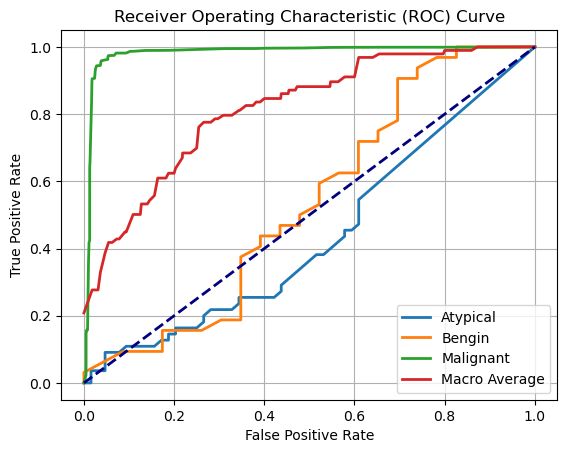
\includegraphics[width=\textwidth]{figures/expirements_and_results/hipt_roc.png}
         \caption{Receiver Operating Characteristic Curve (HIPT)}
     \end{subfigure}
     \hfill
     \begin{subfigure}[b]{0.45\textwidth}
         \centering
         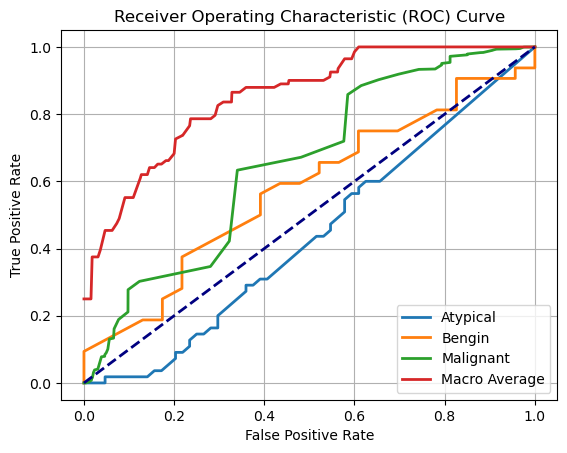
\includegraphics[width=\textwidth]{figures/expirements_and_results/acmil_roc.png}
         \caption{Receiver Operating Characteristic Curve (ACMIL)}
     \end{subfigure}
\end{figure}

\begin{figure}[ht]
     \centering
     \begin{subfigure}[b]{0.45\textwidth}
         \centering
         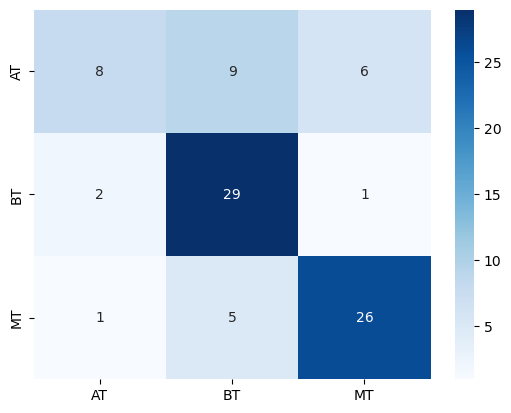
\includegraphics[width=\textwidth]{figures/expirements_and_results/hipt_cm.png}
         \caption{Confusion matrix (HIPT)}
     \end{subfigure}
     \hfill
     \begin{subfigure}[b]{0.45\textwidth}
         \centering
         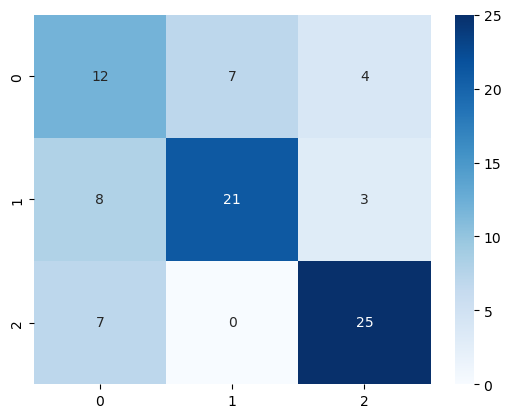
\includegraphics[width=\textwidth]{figures/expirements_and_results/acmil_cm.png}
         \caption{Confusion matrix (ACMIL)}
     \end{subfigure}
\end{figure}

\begin{tikzpicture}
\node[opacity=0.0]{hhh};
\end{tikzpicture}
% \clearpage
\newpage

\section{Information system}
\subsection{Anti Cancer Center}
The Anti Cancer Center of Sidi Bel Abbés (CAC SBA) is one of 25 centers across the country, which are dedicated to the diagnosis and treatment of cancer, it was established in 2017 under the direct supervision of the Algerian Ministry of Health and Population.
\subsection{Objective}
The objective of this collaboration with CAC SBA, is to a create an information system for the purpose of automating data collection and the digitization of patient files. Since everything in their existing system is done manually, introducing an automated system yields many benefits such as:
\begin{itemize}
    \item Saving a considerable amount of time for both patients and medics.
    \item Allowing the medical staff to do statistics and analyse the data very easily.
    \item Facilitating data sharing with other centers.
    \item Enabling the creation of datasets to develop dedicated AI models.
\end{itemize}
\subsection{Overview}

The system is divided into two parts: a web application in which the doctors manage patients files, and an inference desktop application in which the doctor uploads a WSI of a breast pathology and makes a prediction using the best AI model amongst our experimentations. \autoref{fig:cd_cac} represents the class diagram of the information system.

\begin{figure}[H]
    \centering
    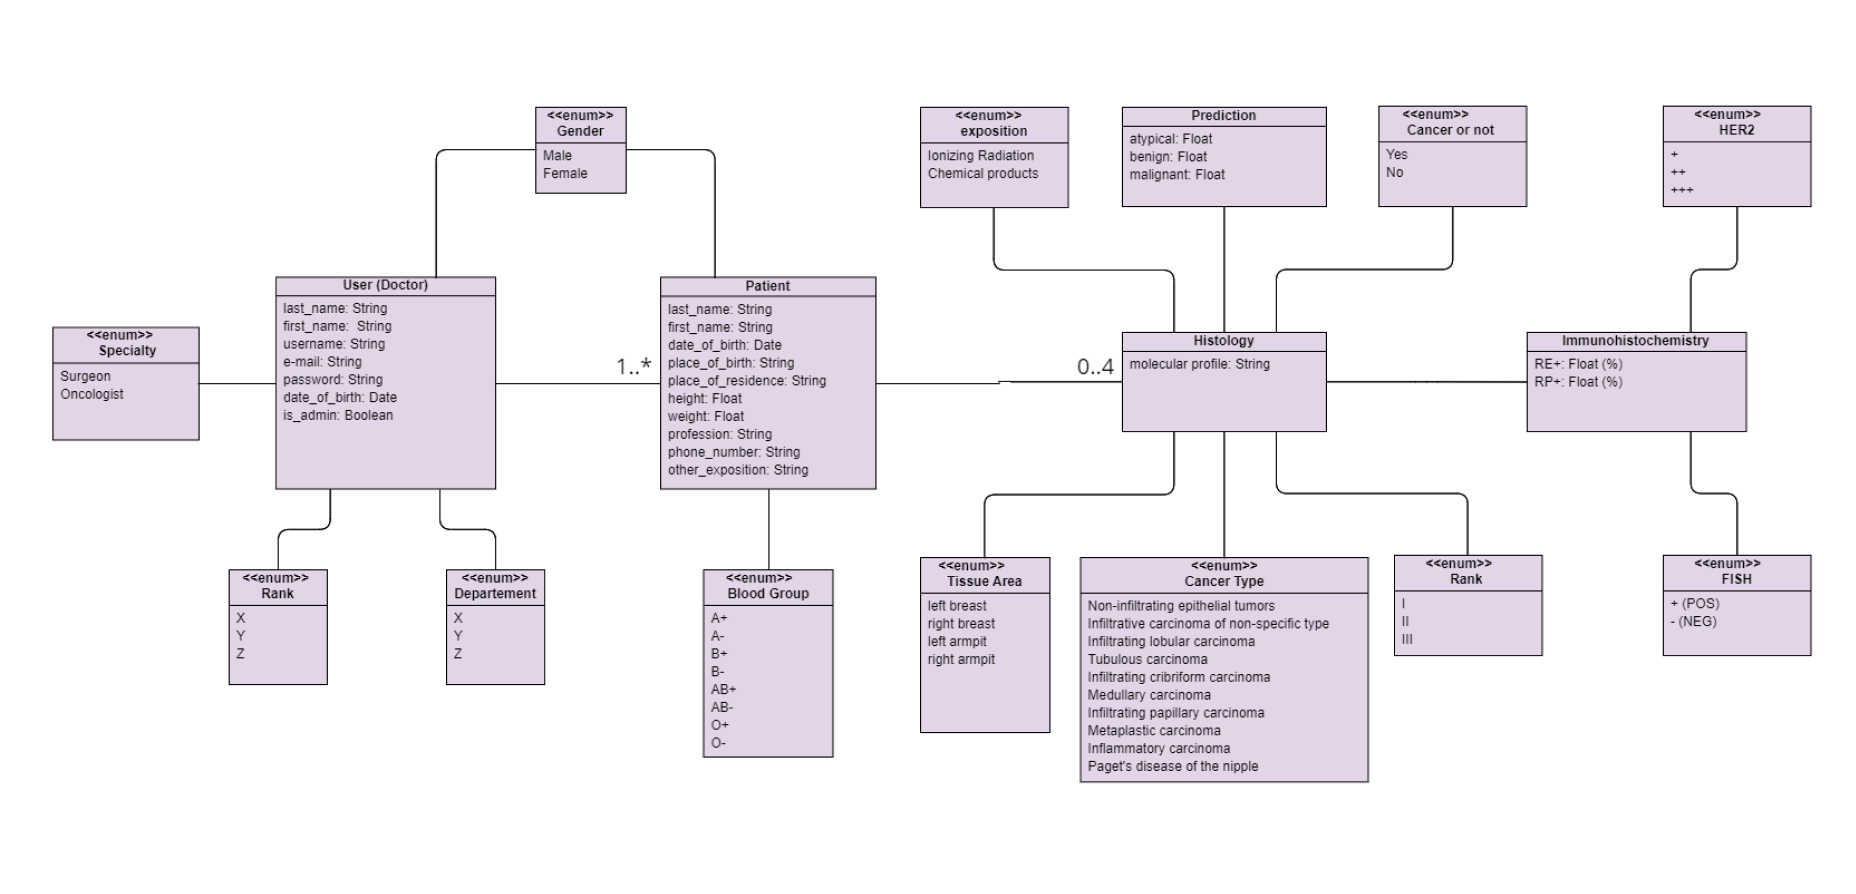
\includegraphics[width=1\linewidth]{figures/SI/cd_cac.png}
    \caption{Class Diagram of the information System}
    \label{fig:cd_cac}
\end{figure}
\subsubsection{Web application}
The web application serves as the primary interface for data collection and managing patient information, it has two principal actors: an Admin and a Doctor. \\

\noindent \textbf{Admin: } The Admin is responsible for managing the system's users, specifically the doctors. Admin tasks include creating, modifying, deleting, and restoring doctors' passwords when necessary. \\

\noindent \textbf{Doctor:} The Doctor is the main user of the system, responsible for managing patient files. They can create, modify, and archive patient records, fill in patient information, view AI model prediction results for patients, and access statistical data. The overall use case diagram is shown in \autoref{fig:uc_web}. 

\begin{figure}[H]
    \centering
    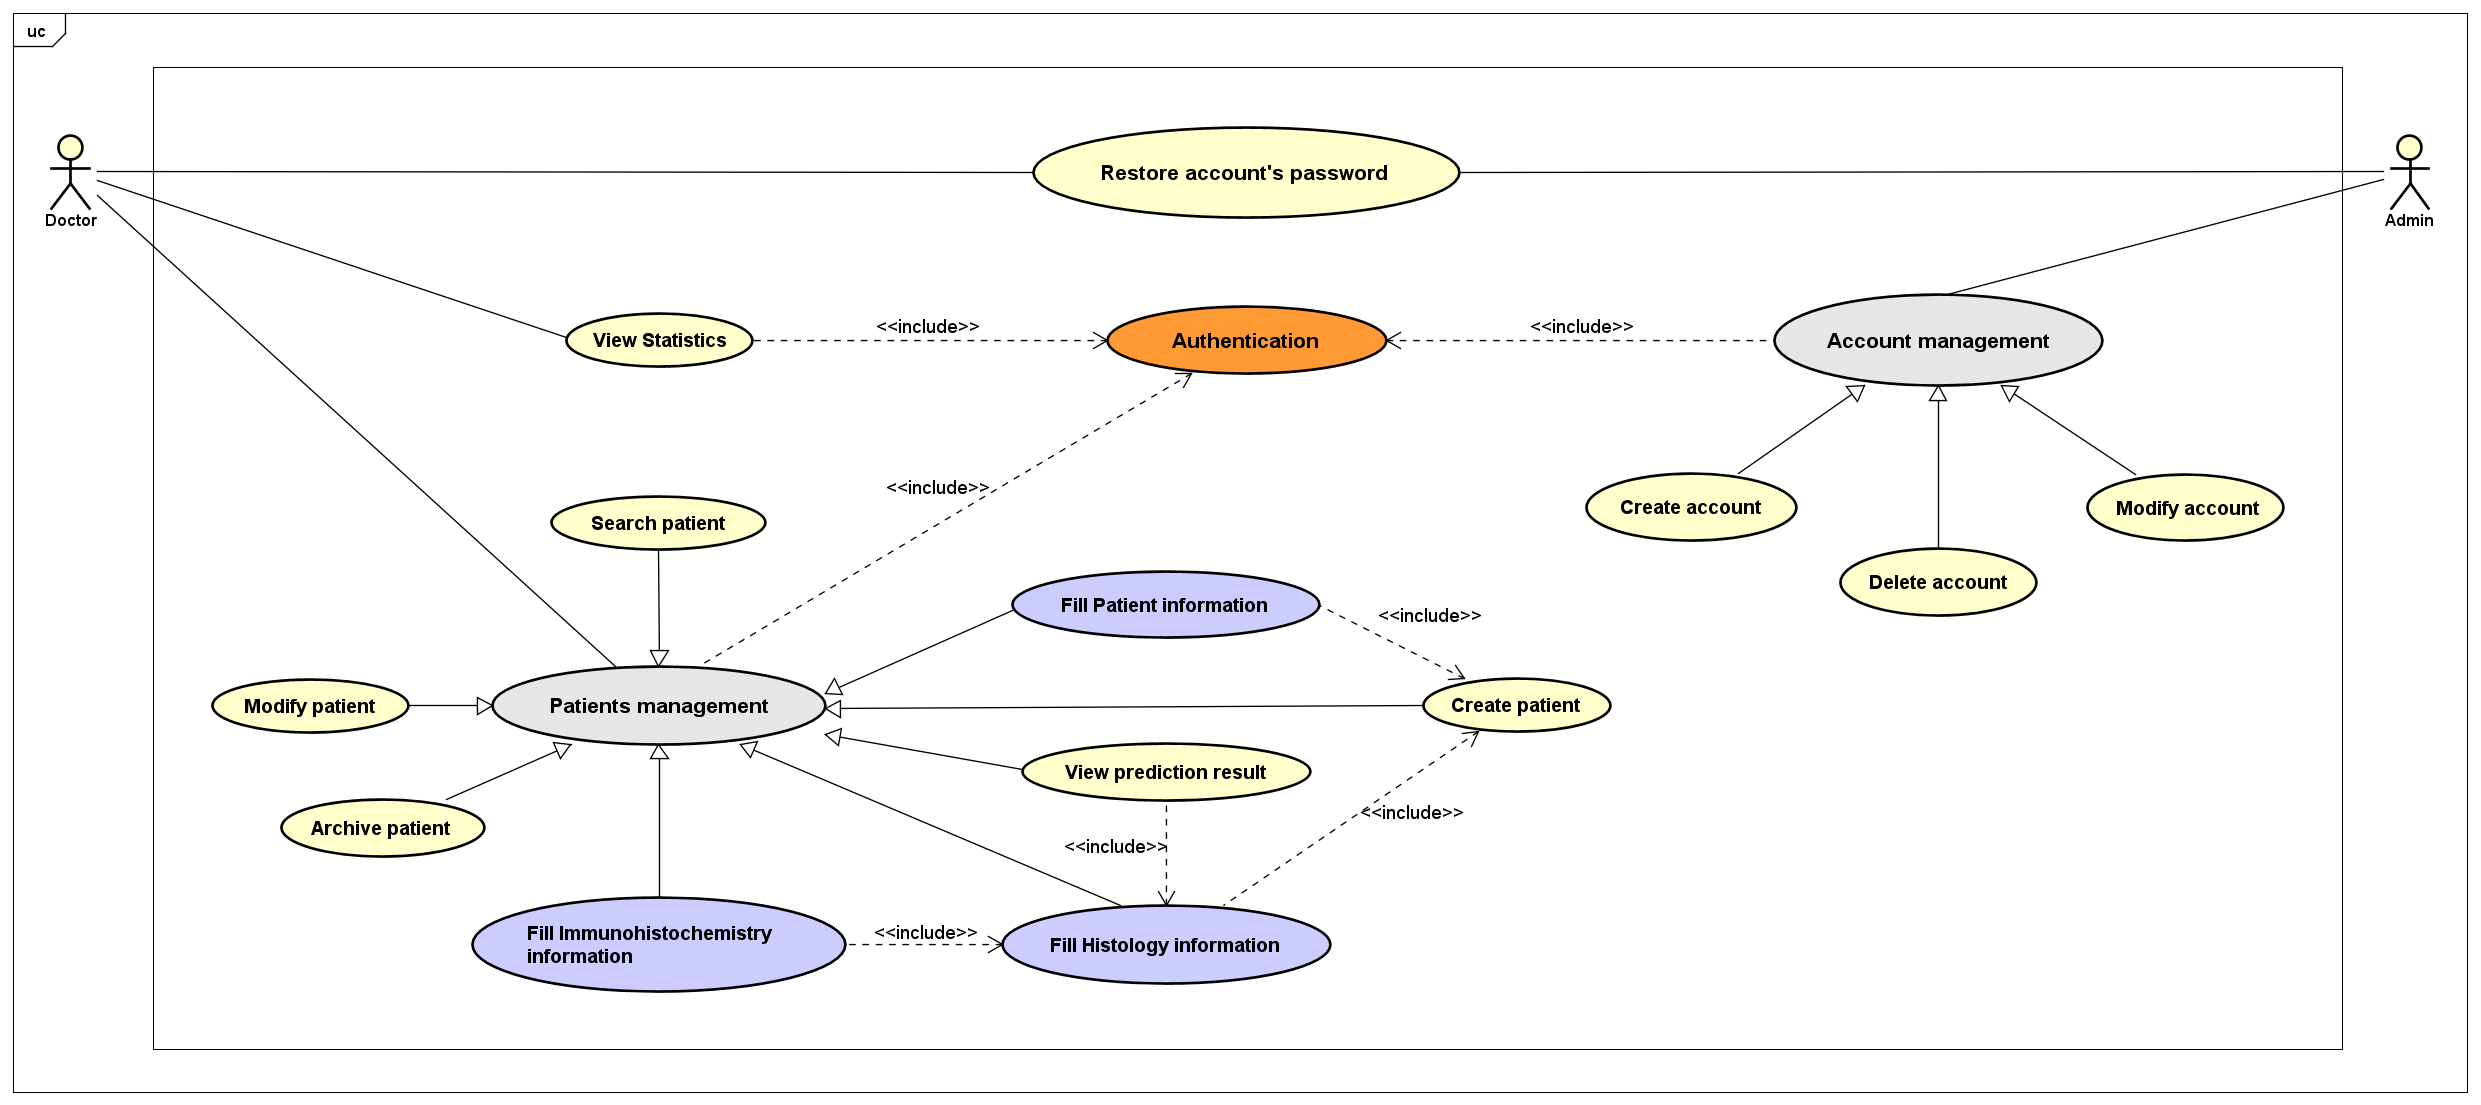
\includegraphics[width=1\textwidth]{figures/SI/uc_website.png}
    \caption{Use Case diagram of the web application}
    \label{fig:uc_web}
\end{figure}

\begin{figure}[H]
    \centering
    \begin{minipage}{0.49\textwidth}
        \centering
        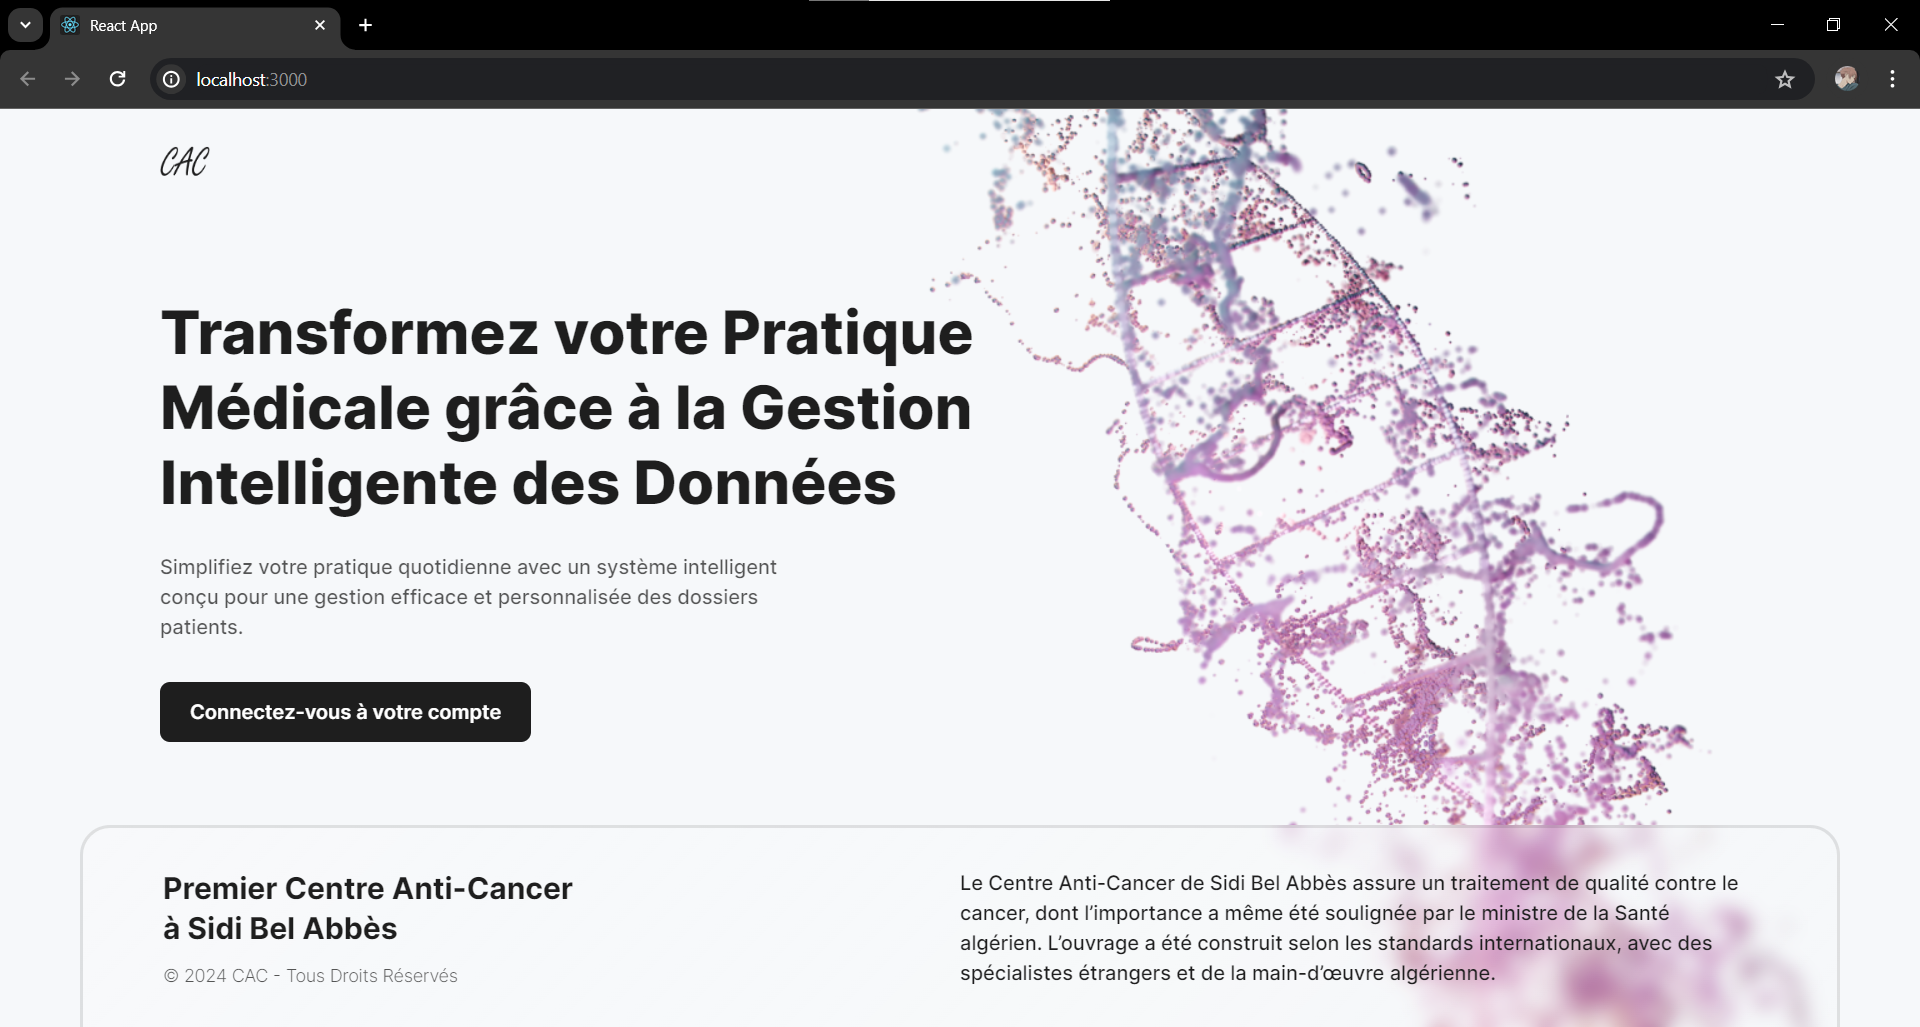
\includegraphics[width=1\linewidth]{figures/SI/web/home.png}
        \caption{Home page}
        \label{fig:home}
    \end{minipage}
    \hfill
    \begin{minipage}{0.49\textwidth}
        \centering
        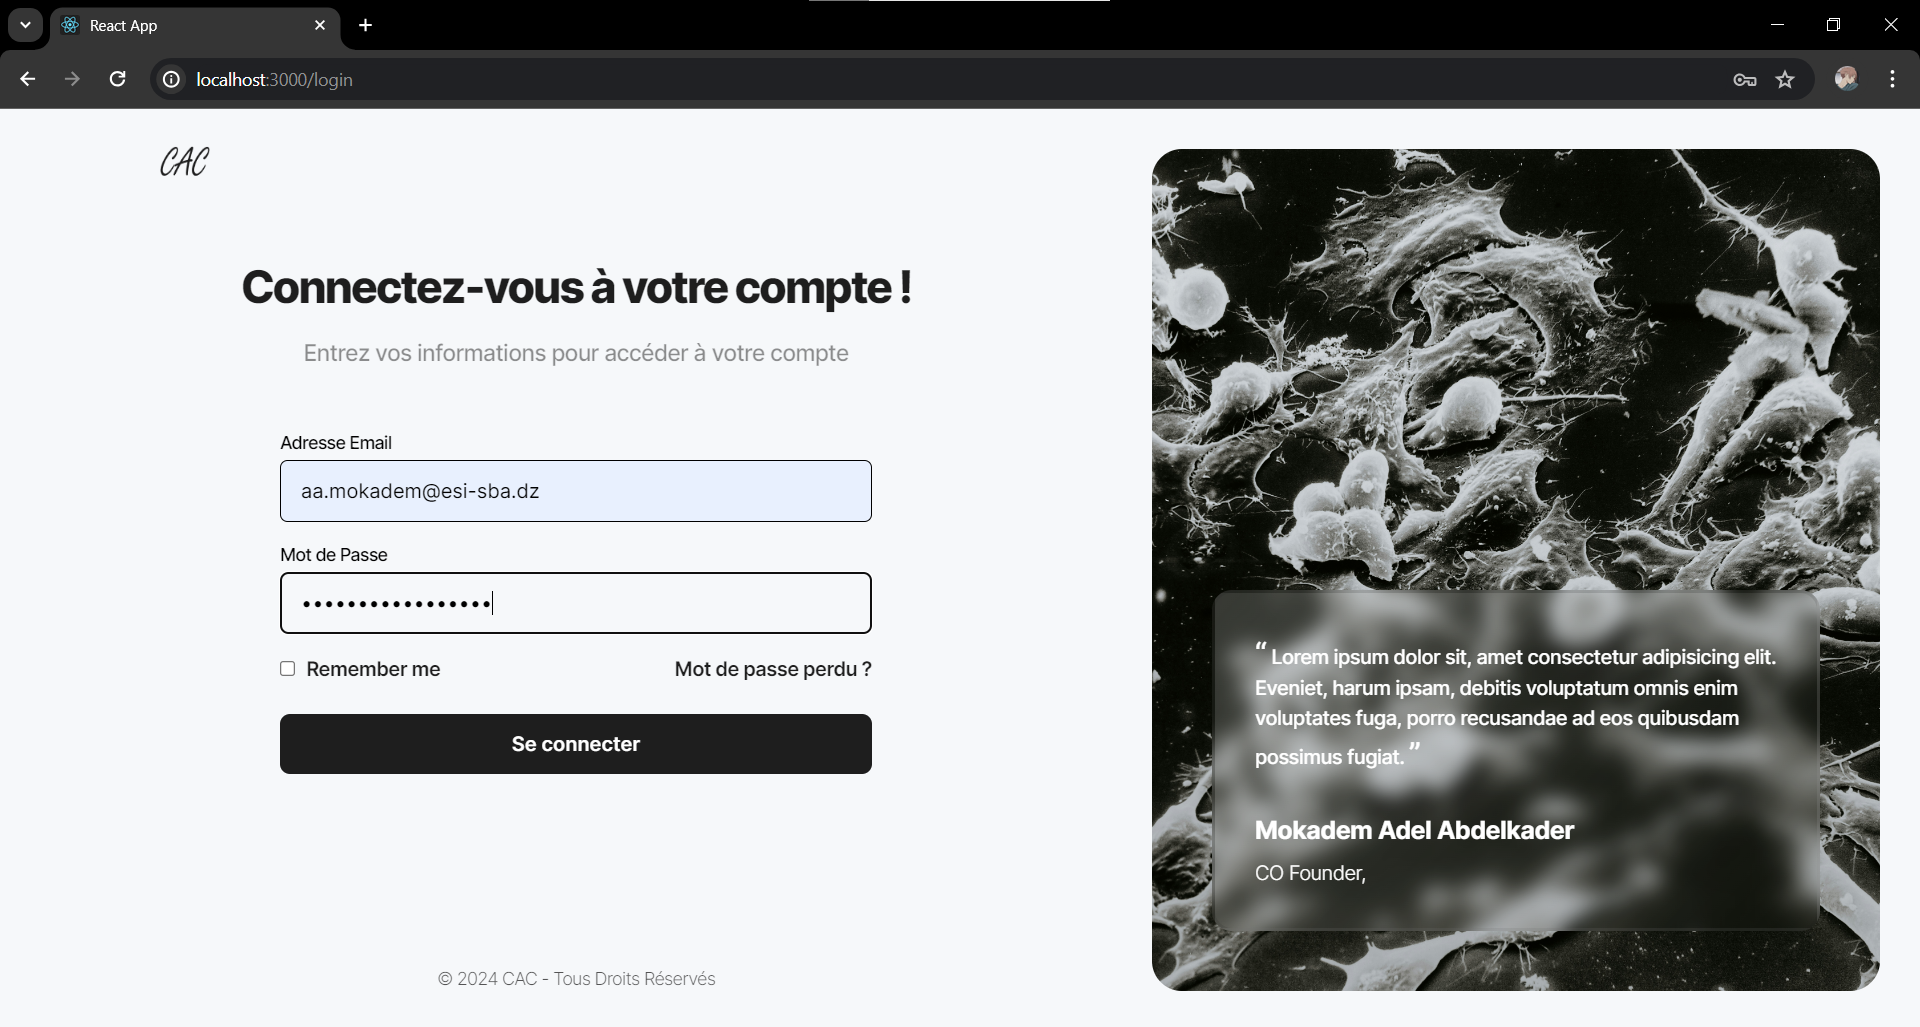
\includegraphics[width=1\linewidth]{figures/SI/web/signin.png}
        \caption{Login page}
        \label{fig:signin}
    \end{minipage}
\end{figure}

\begin{figure}[H]
    \centering
    \begin{minipage}{0.49\textwidth}
        \centering
        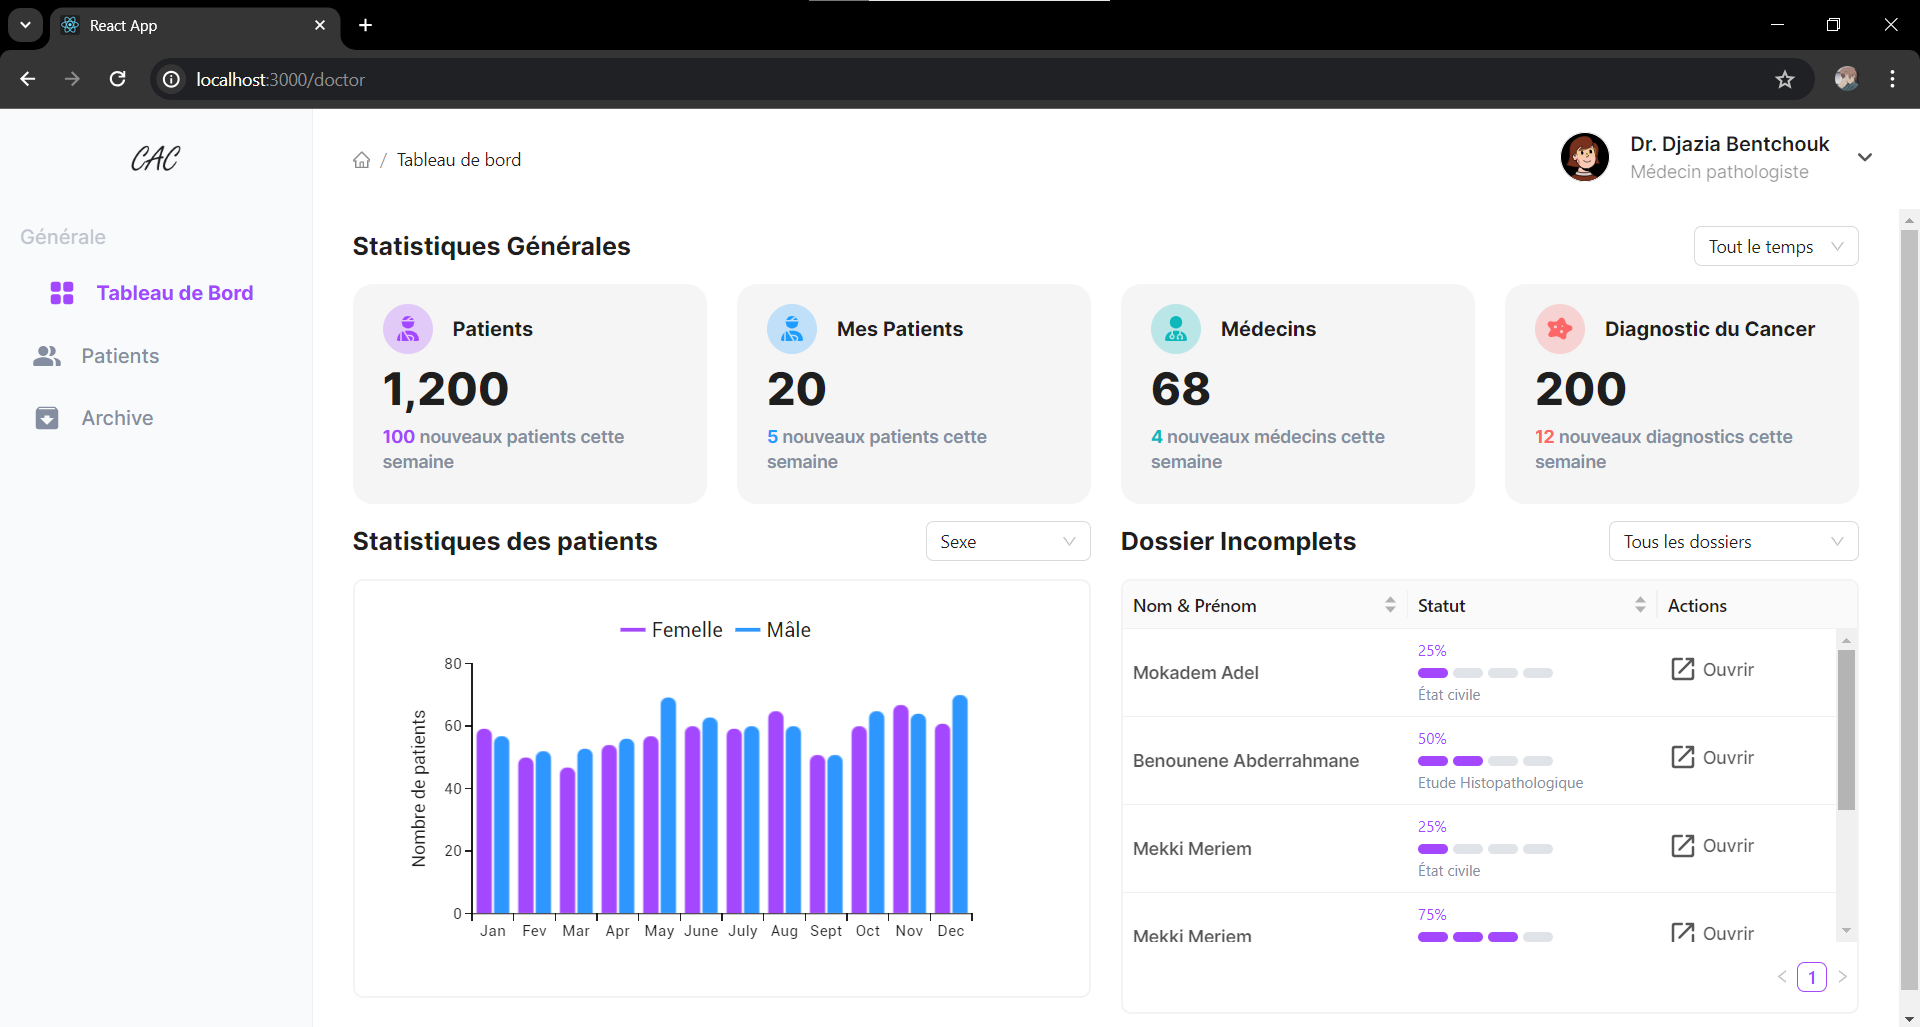
\includegraphics[width=1\linewidth]{figures/SI/web/dashboard.png}
         \caption{Dashboard page}
        \label{fig:dashboard}
    \end{minipage}
    \hfill
    \begin{minipage}{0.49\textwidth}
        \centering
         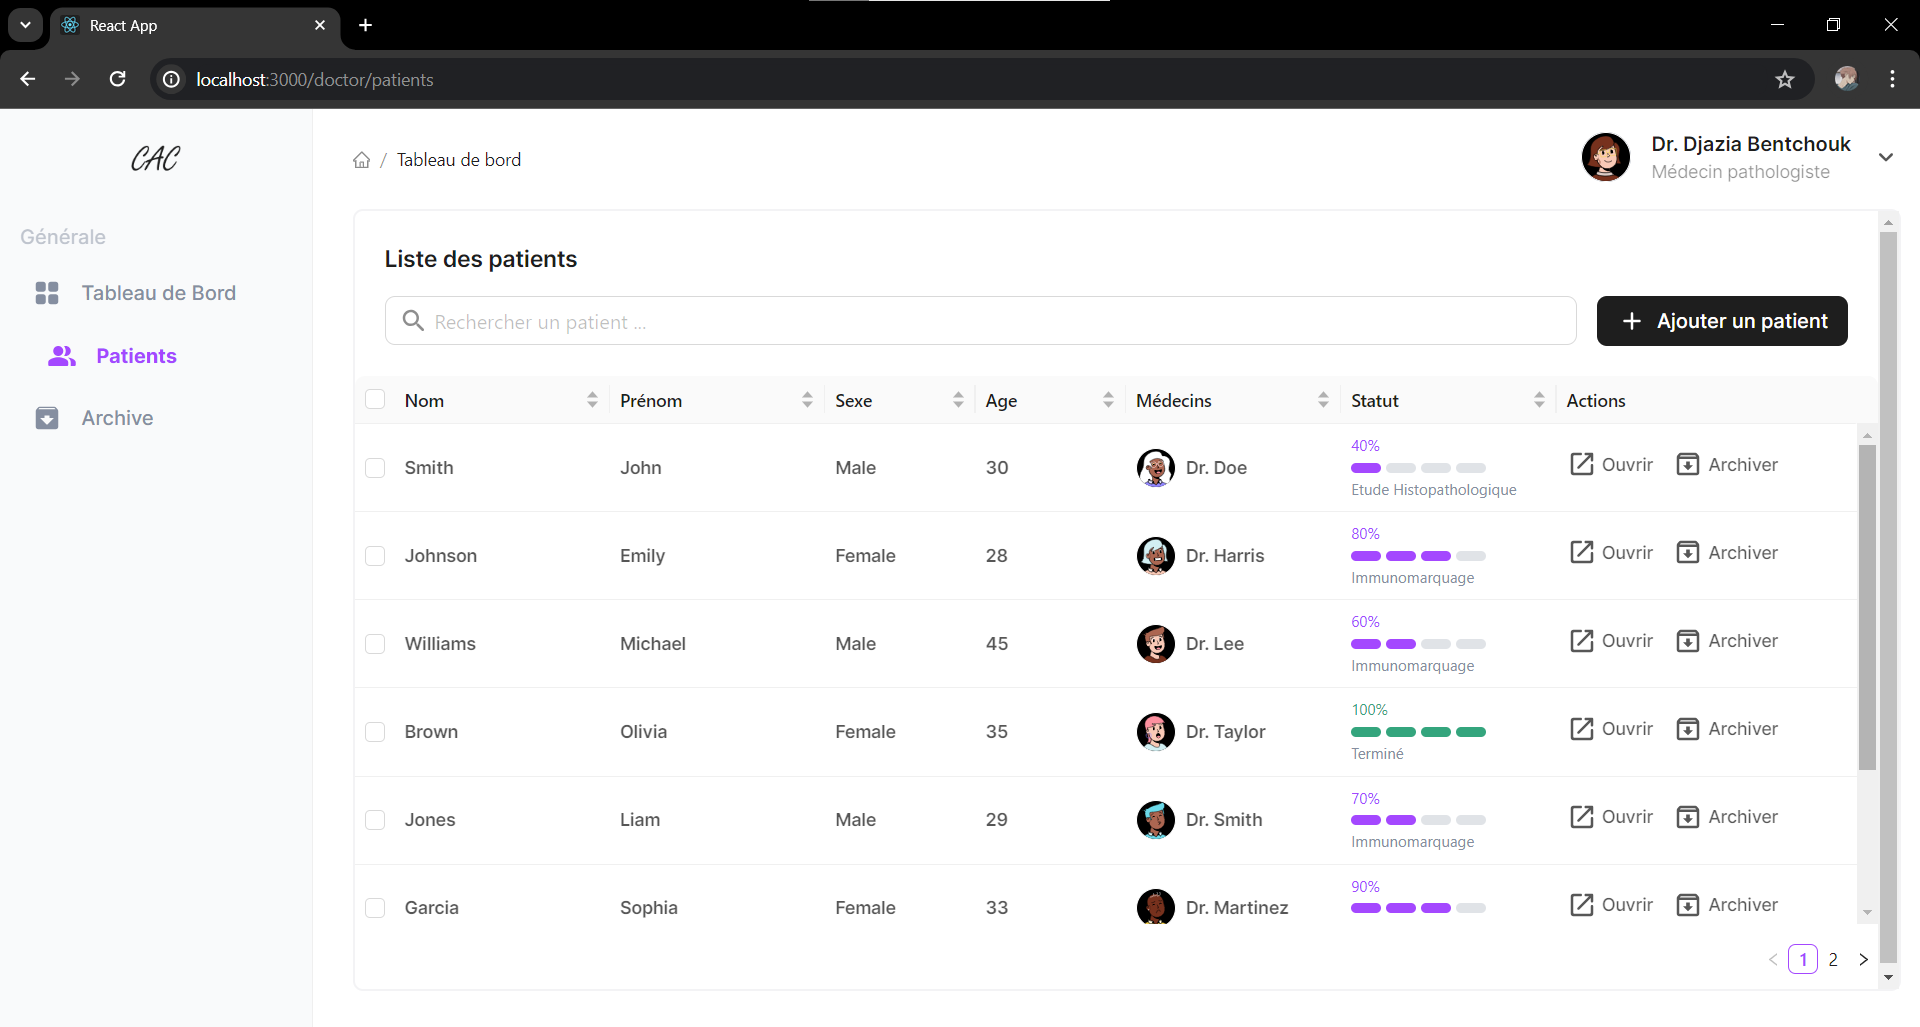
\includegraphics[width=1\linewidth]{figures/SI/web/patients.png}
        \caption{Patients list page}
        \label{fig:patients}
    \end{minipage}
\end{figure}

\begin{figure}[H]
    \centering
    \begin{minipage}{0.49\textwidth}
        \centering
        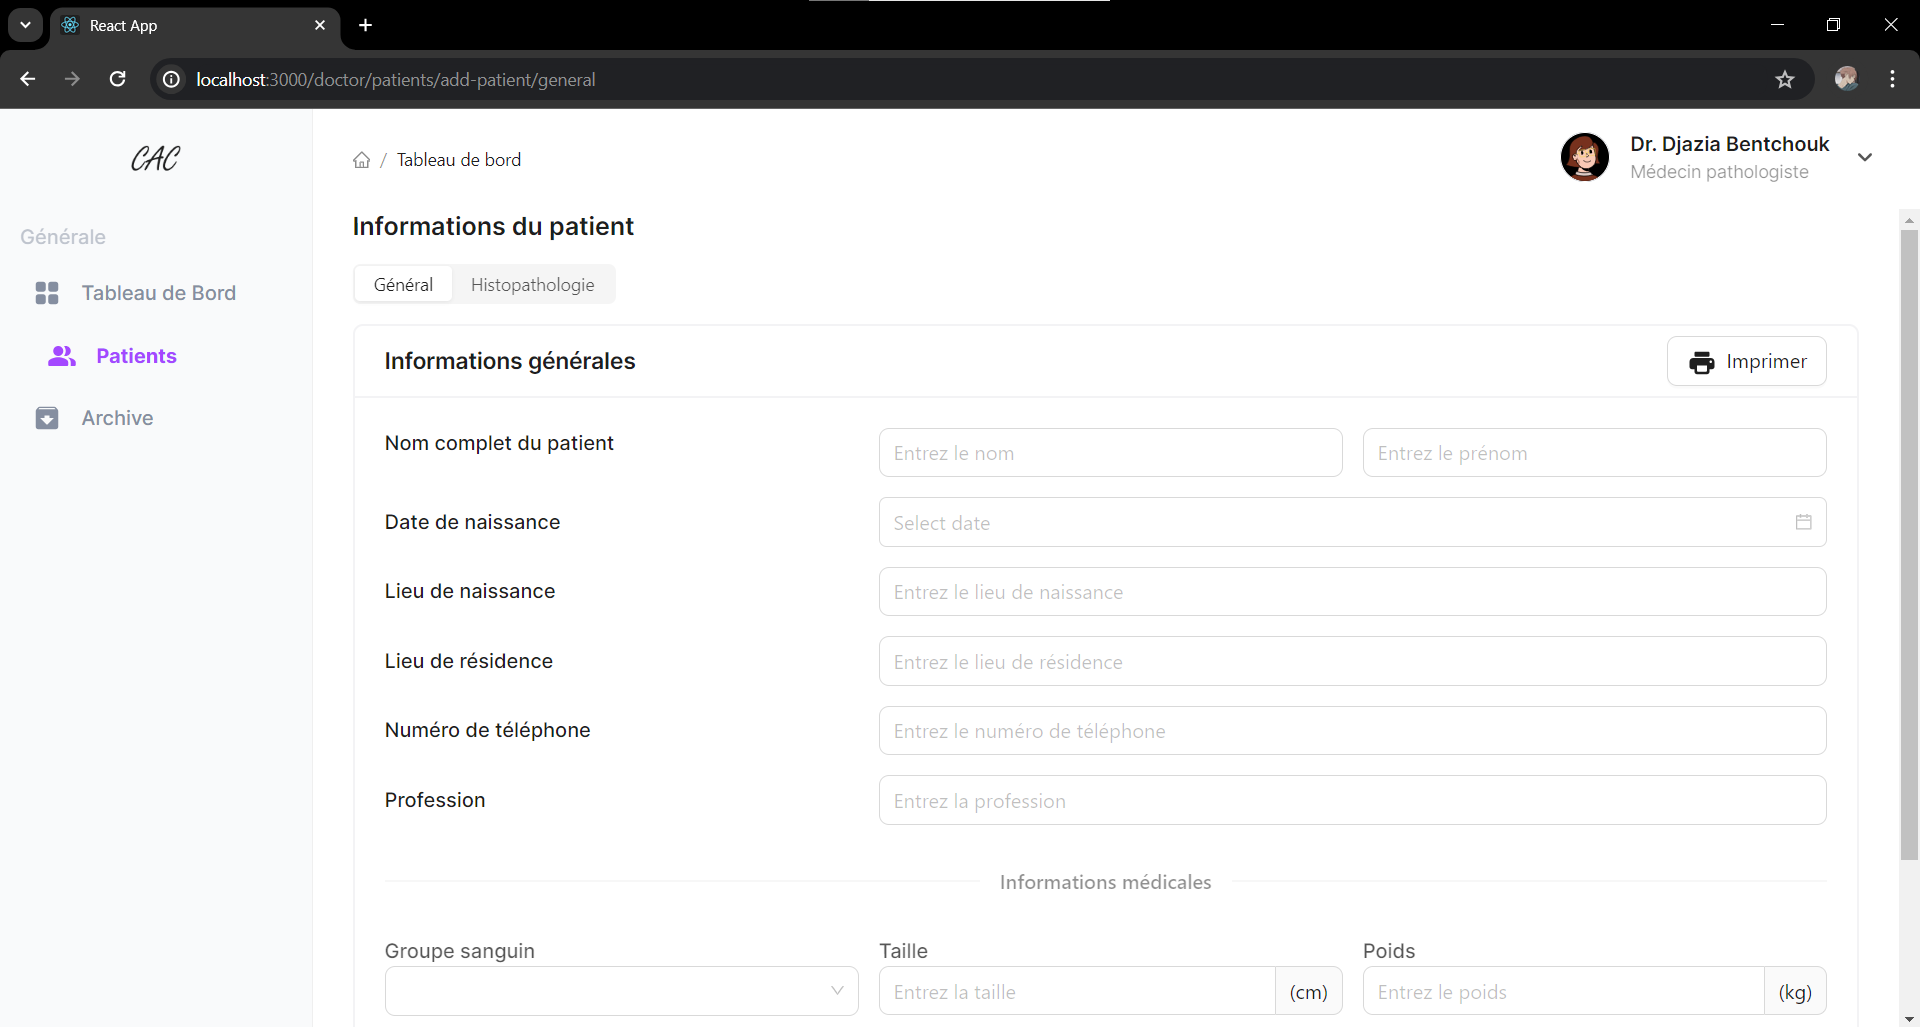
\includegraphics[width=1\linewidth]{figures/SI/web/patient info.png}
        \caption{Patient information form}
        \label{fig:patient_info}
    \end{minipage}
    \hfill
    \begin{minipage}{0.49\textwidth}
        \centering
        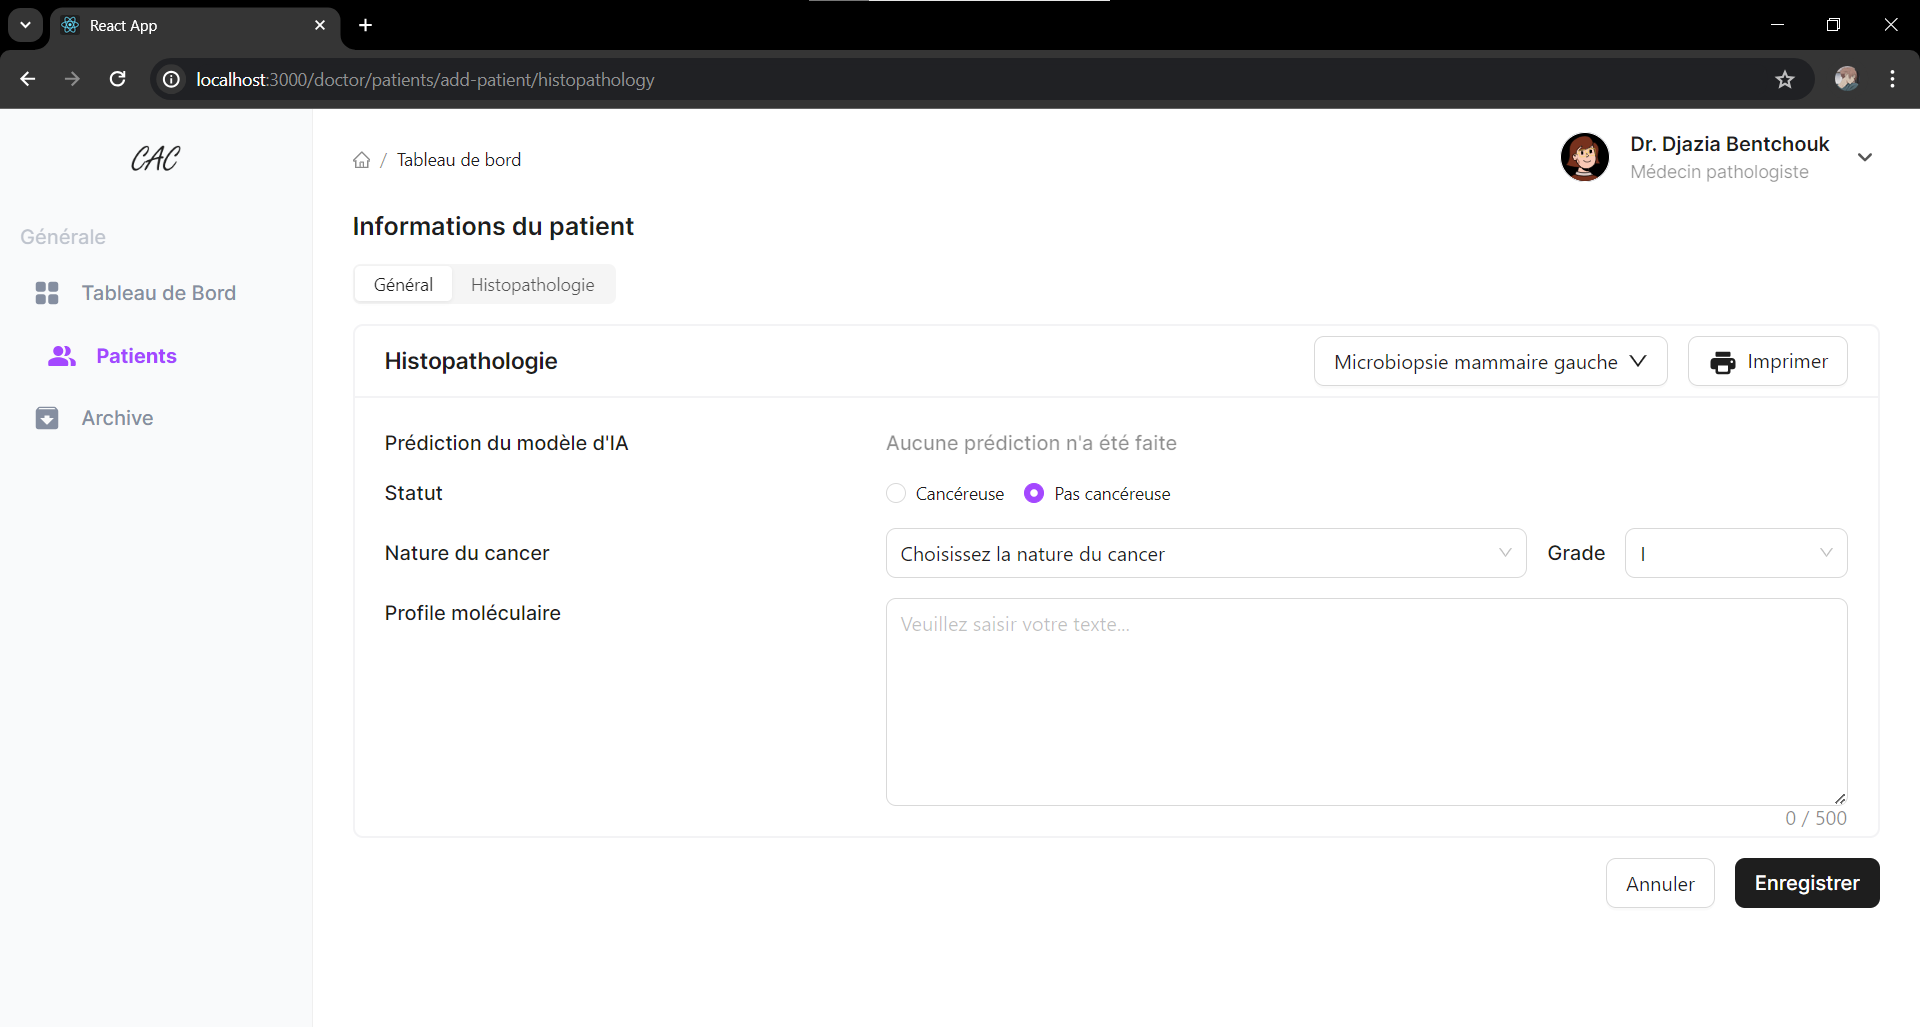
\includegraphics[width=1\linewidth]{figures/SI/web/histo.png}
        \caption{Patient's histology form}
        \label{fig:histo}
    \end{minipage}
\end{figure}

\begin{figure}[H]
    \centering
    \begin{minipage}{0.49\textwidth}
        \centering
        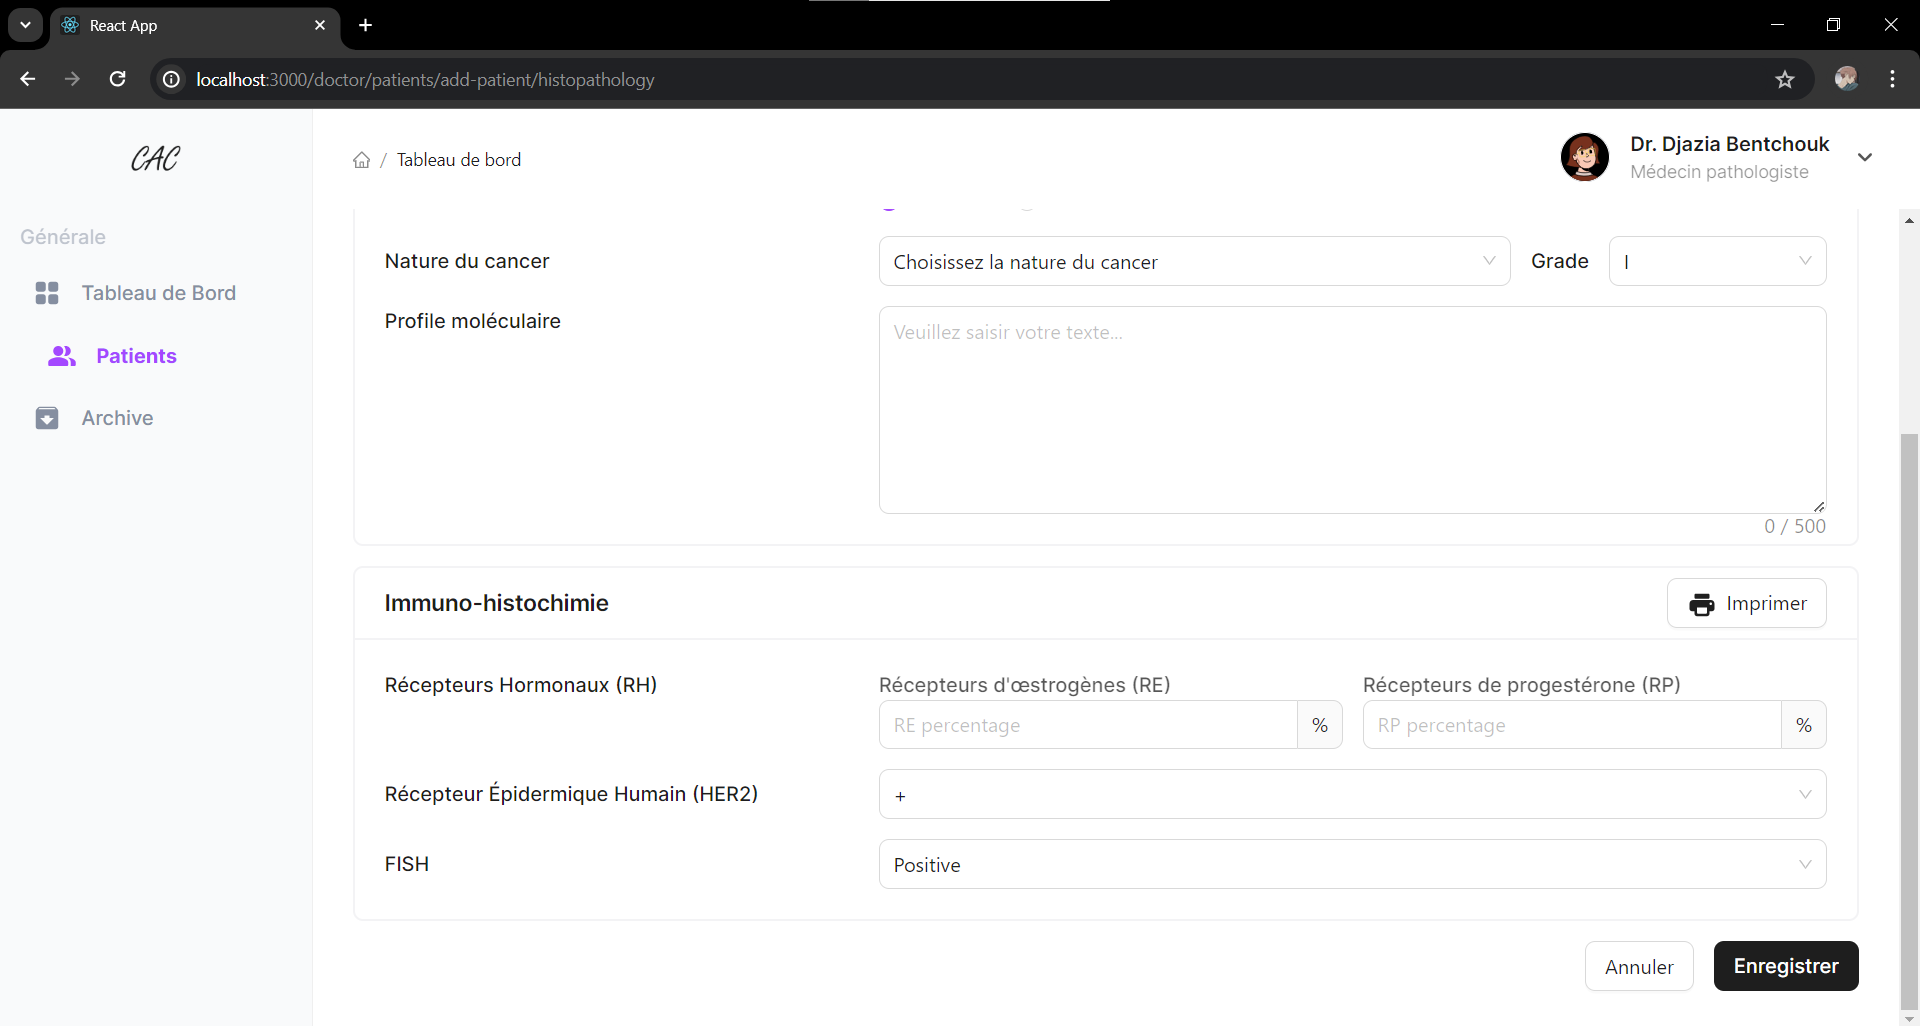
\includegraphics[width=1\linewidth]{figures/SI/web/immuno.png}
        \caption{Patient's immunohistochemistry form}
        \label{fig:immuno}
        
    \end{minipage}
    \hfill
    \begin{minipage}{0.49\textwidth}
        \centering
        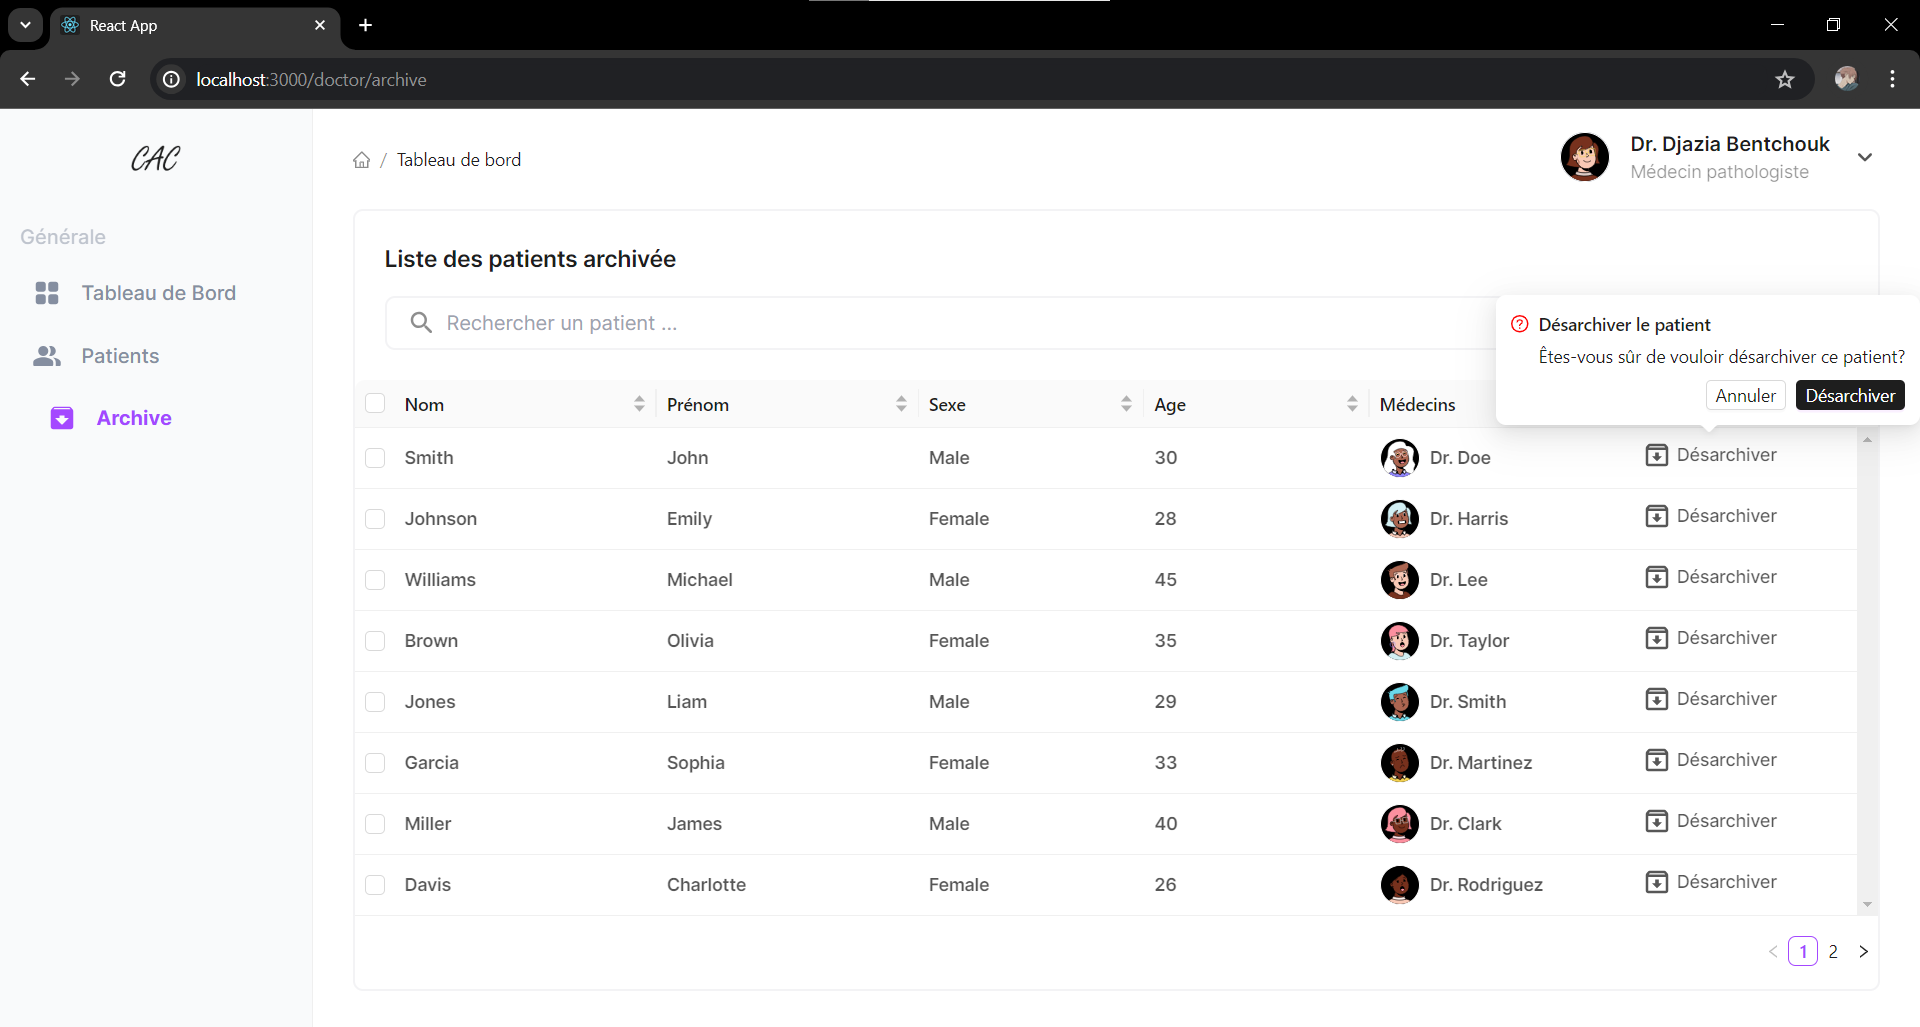
\includegraphics[width=1\linewidth]{figures/SI/web/archive.png}
        \caption{Archived patients page}
        \label{fig:archive}
    \end{minipage}
\end{figure}

\subsubsection{Inference application}
The inference application is designed for making predictions on histology biopsies of specific patients. Doctors can search for a patient, select an available histology, and then upload a WSI to obtain a prediction.

\begin{figure}[H]
    \centering
    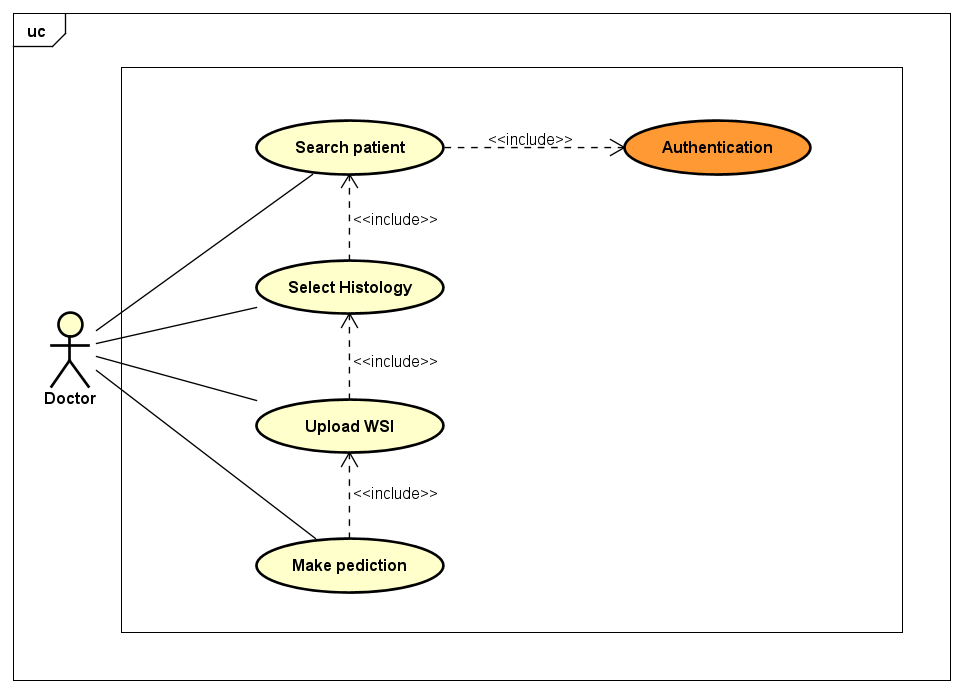
\includegraphics[width=0.7\textwidth]{figures/SI/uc_app.png}
    \caption{Use Case diagram of the inference application}
    \label{fig:uc_desktop}
\end{figure}

\begin{figure}[H]
    \centering
    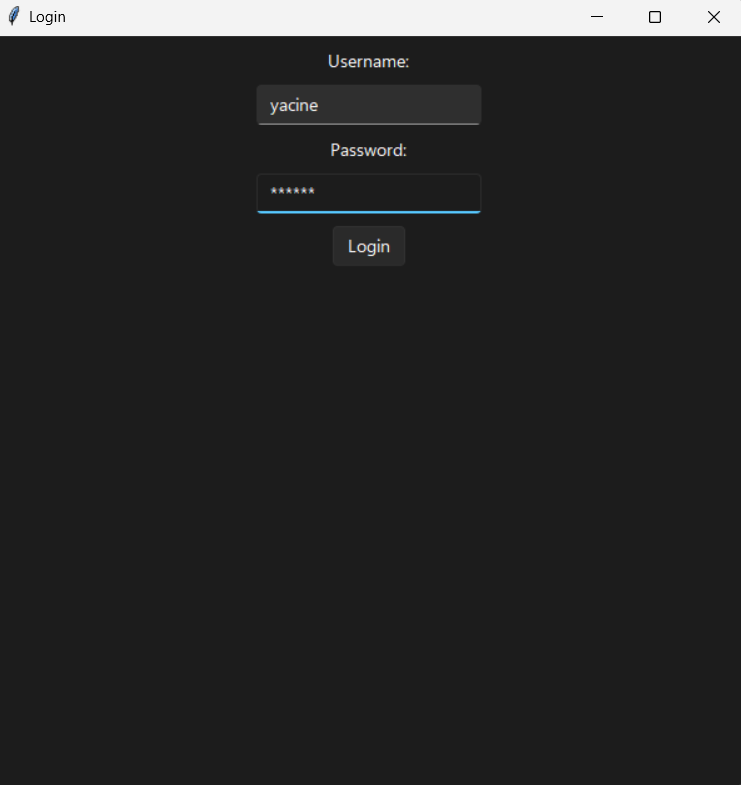
\includegraphics[width=0.75\linewidth]{figures/SI/desktop/login.png}
    \caption{Login page}
    \label{fig:app_login}
\end{figure}

\begin{figure}[H]
    \centering
    \begin{minipage}{0.49\textwidth}
        \centering
        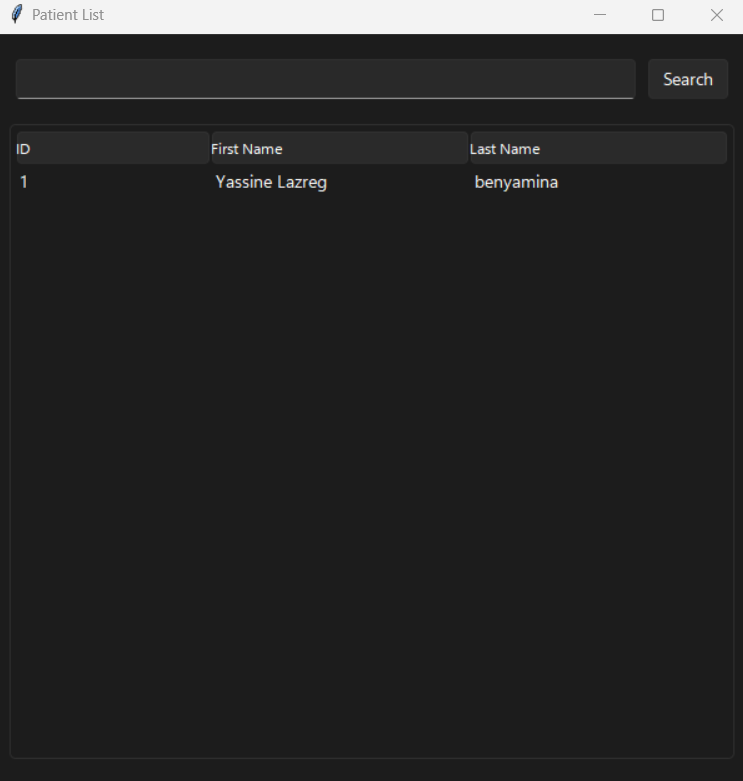
\includegraphics[width=1\linewidth]{figures/SI/desktop/patient_list.png}
        \caption{Doctor's patients list page}
        \label{fig:app_patient_list}
    \end{minipage}
    \hfill
    \begin{minipage}{0.49\textwidth}
        \centering
        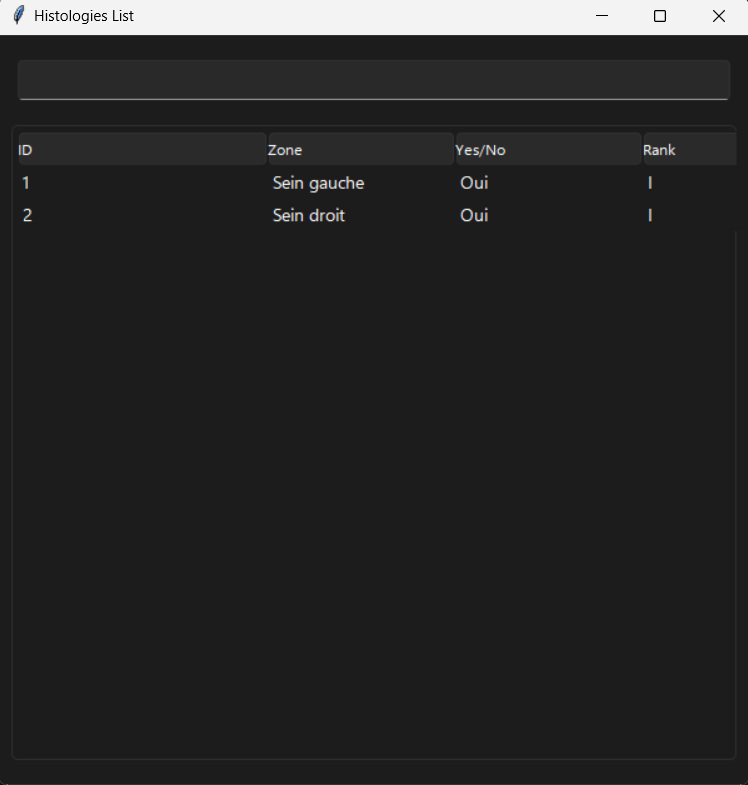
\includegraphics[width=1\linewidth]{figures/SI/desktop/histo_list.png}
        \caption{Patient's histologies list page}
        \label{fig:app_histo_list}
    \end{minipage}
\end{figure}

\begin{figure}[H]
    \centering
    \begin{minipage}{0.49\textwidth}
        \centering
        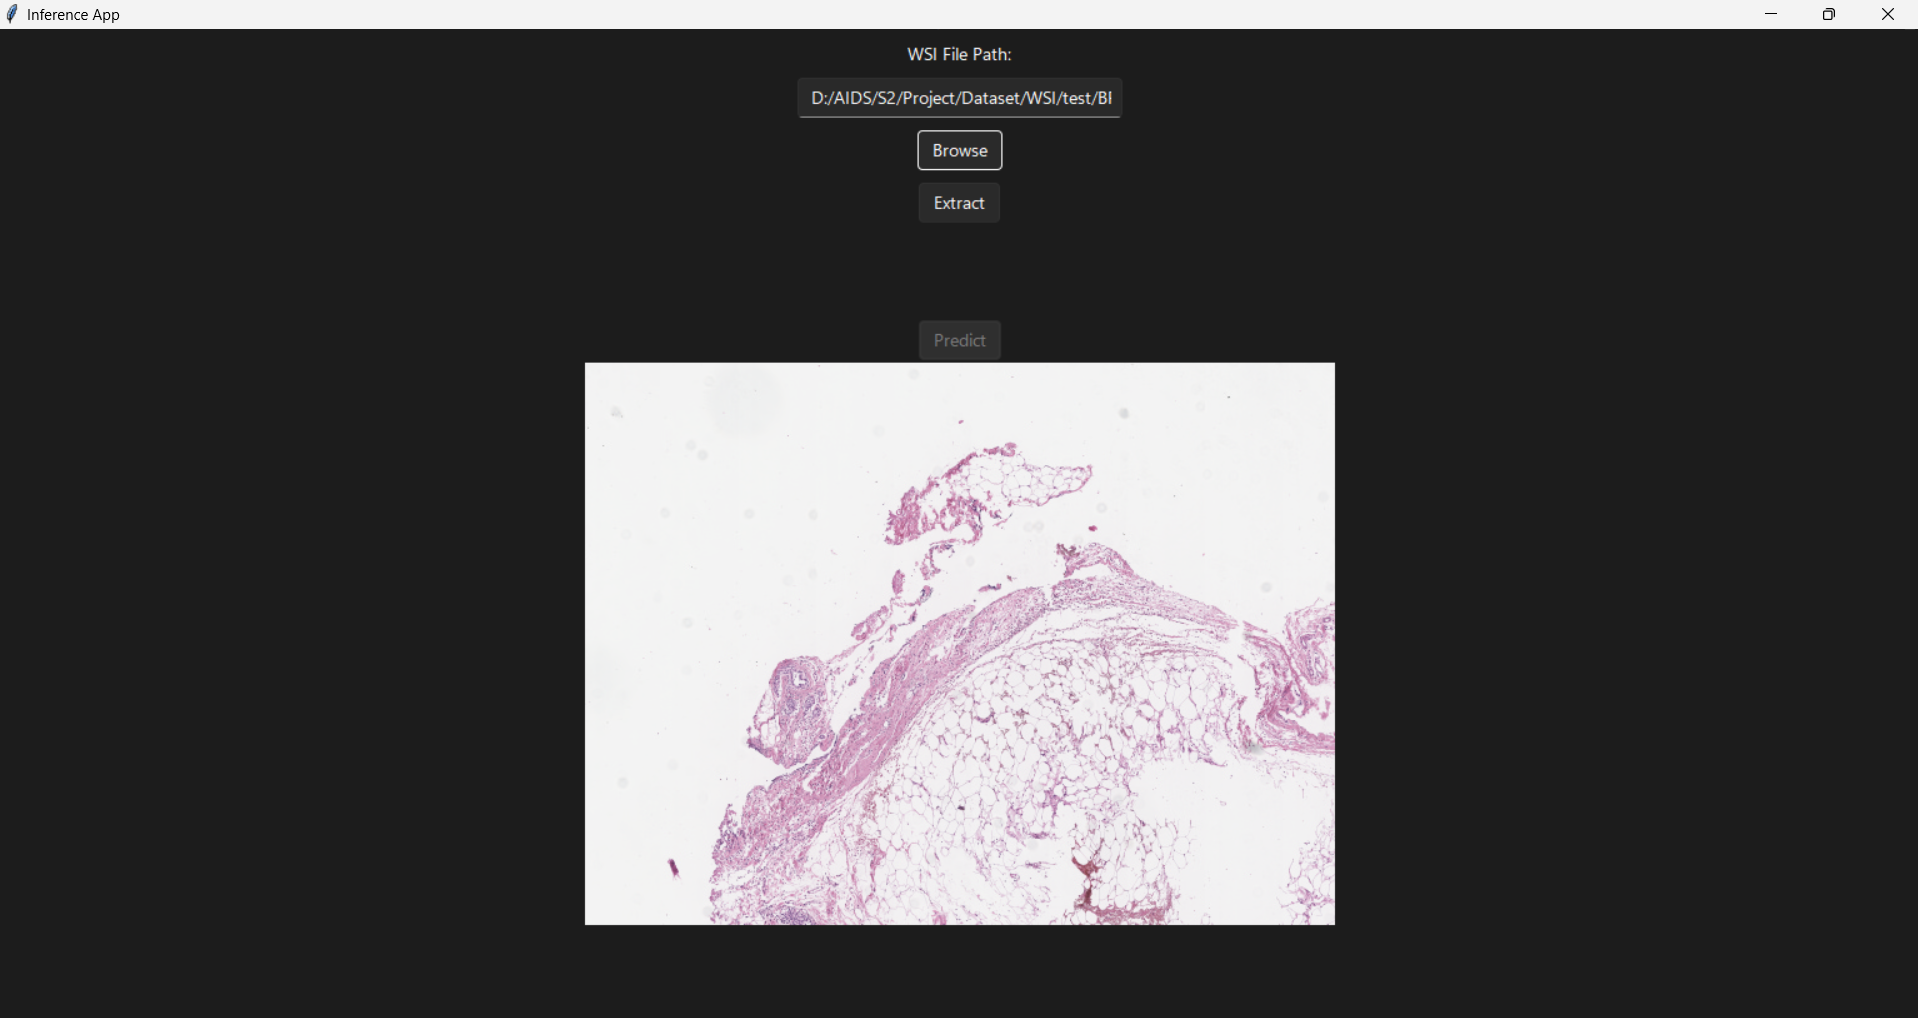
\includegraphics[width=1\linewidth]{figures/SI/desktop/select_wsi.png}
        \caption{Selecting a WSI page}
        \label{fig:app_select_wsi}
    \end{minipage}
    \hfill
    \begin{minipage}{0.49\textwidth}
        \centering
        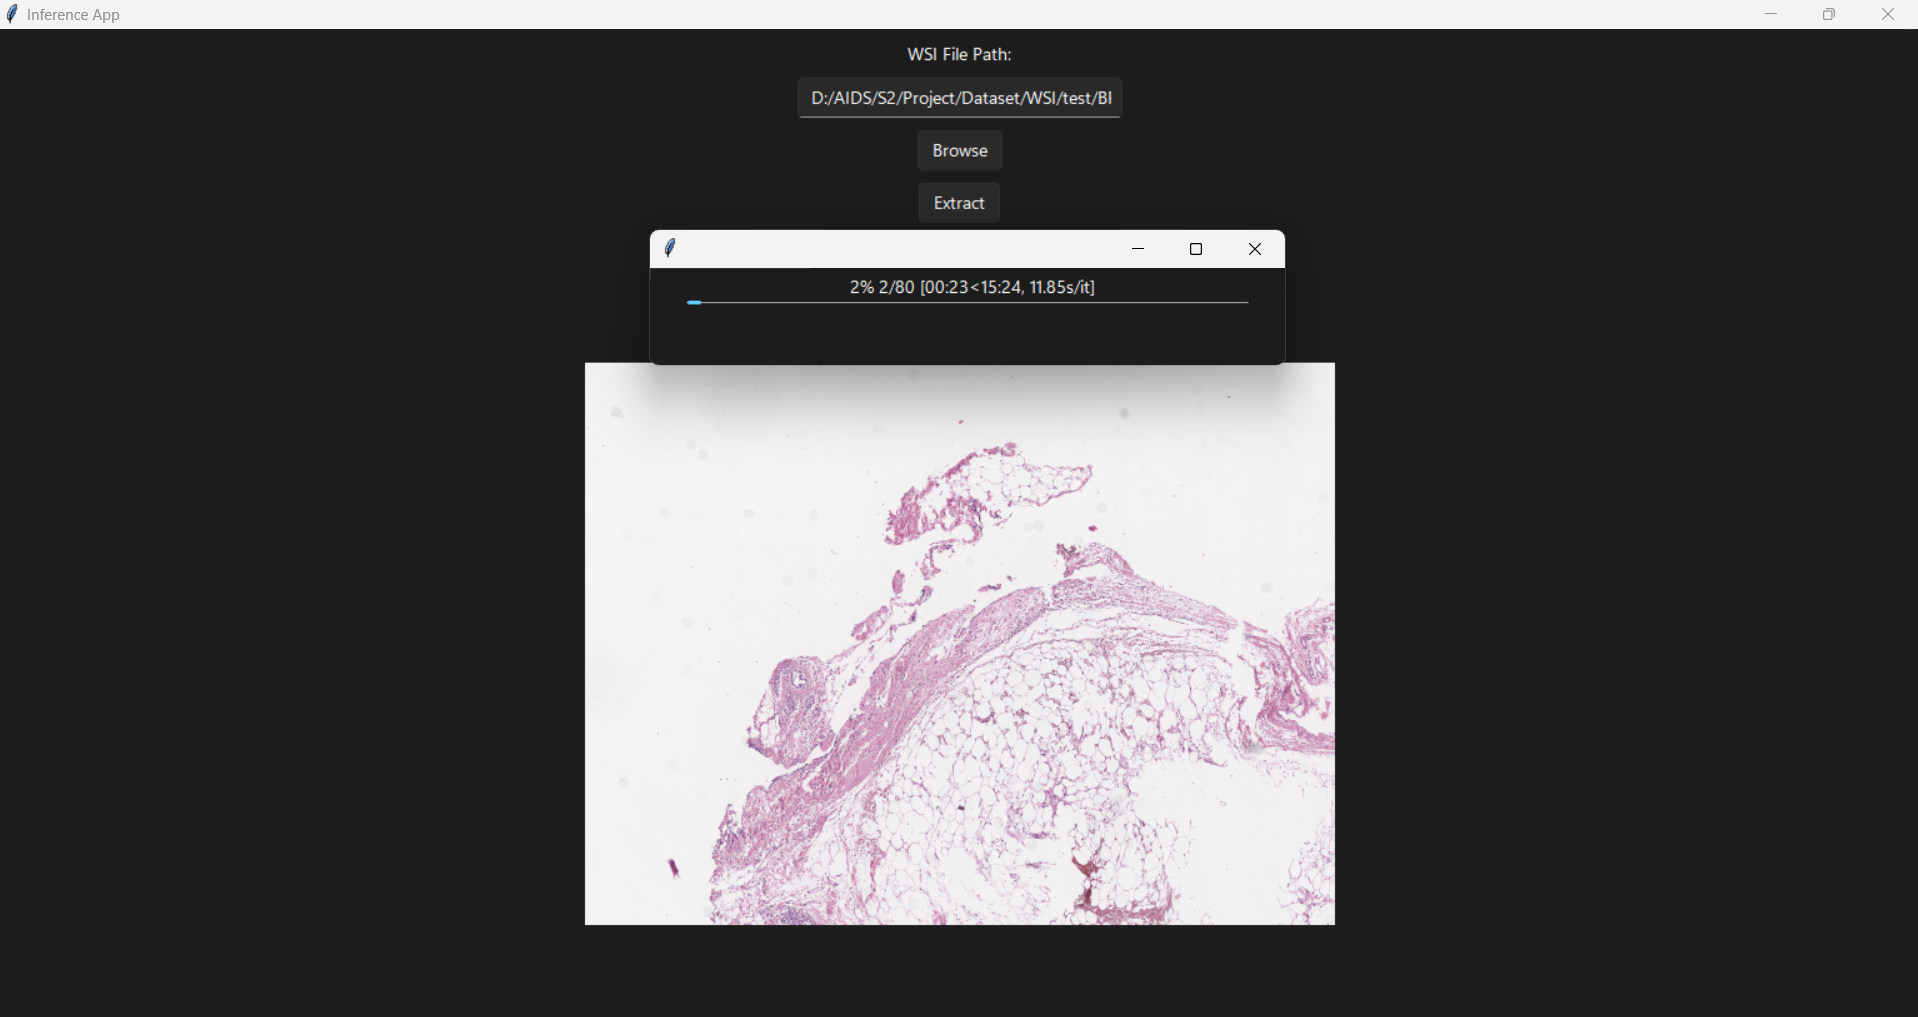
\includegraphics[width=1\linewidth]{figures/SI/desktop/feature_extraction.png}
        \caption{Feature Extraction on the WSI}
        \label{fig:app_feature_extraction}
    \end{minipage}
\end{figure}

\begin{figure}[H]
    \centering
    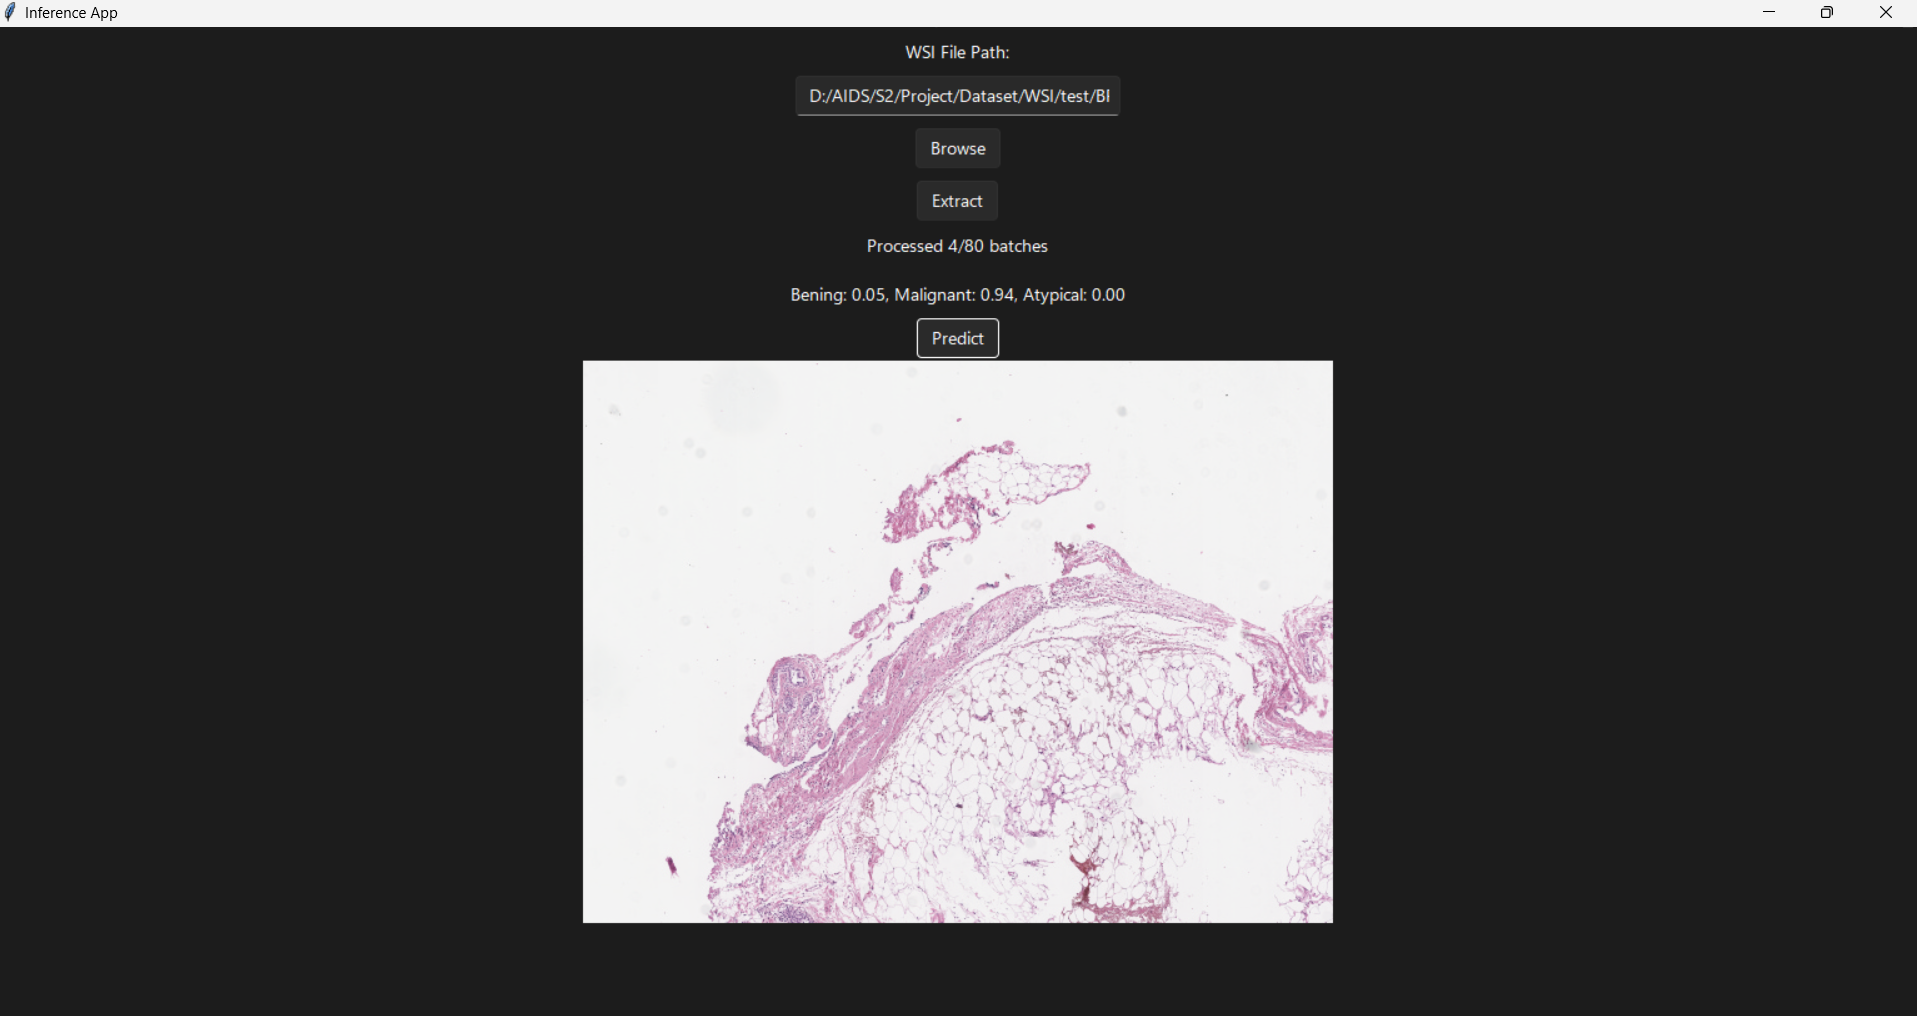
\includegraphics[width=1\linewidth]{figures/SI/desktop/prediction.png}
    \caption{Prediction on the WSI}
    \label{fig:app_pred}
\end{figure}

\newpage
\section{Conclusion}
\noindent This multidisciplinary project aimed to develop an effective and robust system for breast cancer detection in whole slide histopathological images (WSIs), which are complex and high-resolution (gigapixels). A comprehensive approach was employed, utilizing advanced deep learning techniques, cutting-edge model architectures, and data preprocessing and augmentation strategies.\\

\noindent A key component was the use of OpenSlide, a powerful open-source library for processing and manipulating high-resolution WSIs, exploiting the hierarchy of svs files. This tool enabled efficient handling and analysis of the large image files, facilitating the extraction of relevant features for subsequent model training and evaluation.\\

\noindent To enhance feature extraction effectiveness, a fine tuning strategy was employed for the feature extractors. By fine tuning pretrained models on the ROIs from the BRACS dataset, the feature extractors could capture the most salient and discriminative characteristics of the histopathological images, leading to improved performance when applied to the larger WSIs.\\

\noindent The project explored and evaluated diverse deep learning architectures and techniques. Attention-based neural networks, such as those used with ResNet-18, ResNet-34, and the state-of-the-art Vision Transformer (ViT), were employed to leverage the power of self-attention mechanisms in capturing long-range dependencies and spatial relationships within the WSIs.

\noindent Additionally, the Hierarchical Image Processing Transformer (HIPT) model, designed to handle the multi-scale nature of WSIs, was explored. By incorporating data augmentation techniques like rotations, shifts, and flips, the HIPT model exhibited remarkable performance, outperforming the other models across all evaluation metrics except for the AUC.\\

\noindent The project's success can be attributed to the synergistic combination of advanced deep learning architectures, effective data preprocessing and augmentation strategies, and fine tuning of feature extractors. The results demonstrate the potential of these techniques in addressing the challenges of breast cancer detection in histopathological images, paving the way for more accurate and reliable diagnostic tools, taking the load off doctors.\\

\noindent Deploying such a system in real-world clinical settings would require rigorous validation and testing to ensure robustness and reliability across diverse patient populations and imaging protocols. Collaboration with domain experts, such as pathologists and oncologists, would be crucial in refining the system and addressing any potential biases or limitations.\\

\noindent Ultimately, the successful implementation of this breast cancer detection system could have far-reaching implications, empowering healthcare professionals with a powerful tool for early detection and accurate diagnosis, potentially leading to improved patient outcomes and more effective treatment strategies.\\

\noindent Moreover, the collaboration with the Anti Cancer Center of Sidi Bel Abbés (CAC SBA) demonstrates the critical role of a well-structured information system in healthcare. By automating data collection and digitizing patient files, the system not only enhances efficiency but also enables comprehensive data analysis, facilitates data sharing with other centers, and supports the development of AI models. This integrated approach represents a significant step forward in modernizing cancer diagnosis and treatment, promising considerable benefits for both medical staff and patients.

\noindent However, we do not intend to stop here. In the future, we aim to leverage Vision Mamba \cite{VIM}, a new architecture that is said to replace transformers due to its performance and computational efficiency. By exploring this novel and potentially revolutionary architecture, we strive to remain at the forefront of technological advancements, continuing to improve our breast cancer detection system. This proactive approach ensures that we stay ahead of the curve and contribute significantly to the field of medical AI.

% Increment the section counter manually
\stepcounter{section}

% Continue writing here ...
\newpage
\section*{References}
\addcontentsline{toc}{section}{\numberline{\thesection}References}

\nocite{ACMIL}
\nocite{BRACS_DATASET}
\nocite{Gigapixel}
\nocite{HIPT}
\nocite{ResNet-OG}
\nocite{FTvsTL}
\nocite{FTandTL}
\nocite{CLAM}
\nocite{Vit}
\nocite{CNNs}
\nocite{CNNs-GFG}
\nocite{CNNs-stanford}
\nocite{Att-Computer-Vision}
\nocite{DINO}
\nocite{Structered-DL-Model}
\nocite{Classification_of_BRCA_hist_CNN}
\nocite{brca-resnet-finetuning}
\nocite{DIETTERICH199731}
\nocite{BreakHis_DATASET}
\nocite{BIOIMAGING}
\nocite{SE-RESNET}
\nocite{BATCH}
\nocite{VIM}
\nocite{NIPS1990_e46de7e1}
\nocite{AttIsAllYouNeed}

\Urlmuskip=0mu plus 1mu
\printbibliography[heading=none]

\iffalse
\glsaddall
\printglossaries
\fi


\end{document}